

\documentclass[12pt, a4paper, oneside]{article}

% ------------------------------------------------------------------------------
% ENCODING & LANGUAGE
% ------------------------------------------------------------------------------
\usepackage[utf8]{inputenc}
\usepackage[T1]{fontenc}
\usepackage[english]{babel}
\usepackage{lmodern}
% \usepackage{microtype}

% ------------------------------------------------------------------------------
% FONTS  — matches standard econometrics journals (Times-like serif)
% ------------------------------------------------------------------------------

\usepackage[scaled=0.90]{helvet}
\usepackage{courier}

% ------------------------------------------------------------------------------
% PAGE GEOMETRY
% ------------------------------------------------------------------------------
\usepackage[
  a4paper,
  top    = 2.5cm,
  bottom = 2.5cm,
  left   = 2.5cm,
  right  = 2.5cm,
  headheight = 14pt
]{geometry}

% ------------------------------------------------------------------------------
% SPACING
% ------------------------------------------------------------------------------
\usepackage{setspace}
\onehalfspacing          


% ------------------------------------------------------------------------------
% MATHEMATICS
% ------------------------------------------------------------------------------
\usepackage{amsmath, amssymb, amsthm}
\usepackage{bm}                % bold math symbols

% Theorem-like environments
\theoremstyle{plain}
\newtheorem{proposition}{Proposition}[section]
\newtheorem{lemma}[proposition]{Lemma}
\newtheorem{corollary}[proposition]{Corollary}
\theoremstyle{definition}
\newtheorem{definition}[proposition]{Definition}
\newtheorem{remark}[proposition]{Remark}

% Convenient math macros
\newcommand{\E}{\mathbb{E}}
\newcommand{\R}{\mathbb{R}}
\newcommand{\N}{\mathbb{N}}
\newcommand{\Prob}{\mathbb{P}}
\newcommand{\indic}{\mathbf{1}}
\newcommand{\tauhat}{\hat{\tau}}
\newcommand{\phat}{\hat{p}}
\newcommand{\omegavec}{\boldsymbol{\omega}}
\newcommand{\kappavec}{\boldsymbol{\kappa}}
\DeclareMathOperator{\Var}{Var}
\DeclareMathOperator{\Cov}{Cov}
\DeclareMathOperator{\plim}{plim}

% ------------------------------------------------------------------------------
% TABLES & FIGURES
% ------------------------------------------------------------------------------
\usepackage{booktabs}          % publication-quality tables
\usepackage{threeparttable}    % notes below tables
\usepackage{tabularx}
\usepackage{multirow}
\usepackage{graphicx}
\usepackage{float}
% \usepackage{bbm}
\usepackage{caption}
\usepackage{subcaption}
\captionsetup{
  font      = small,
  labelfont = bf,
  format    = hang,
  width     = 0.95\textwidth
}

% ------------------------------------------------------------------------------
% HYPERLINKS & CROSS-REFERENCES
% ------------------------------------------------------------------------------
\usepackage[
  colorlinks = true,
  linkcolor  = black,
  citecolor  = black,
  urlcolor   = black
]{hyperref}
\usepackage{cleveref}

% ------------------------------------------------------------------------------
% BIBLIOGRAPHY  — Author-year (AER/econometrics standard)
% ------------------------------------------------------------------------------
\usepackage[round,authoryear]{natbib}


% ------------------------------------------------------------------------------
% MISC
% ------------------------------------------------------------------------------
% \usepackage{microtype}         % better typography
\usepackage{parskip}           % space between paragraphs instead of indent
\usepackage{enumitem}
\usepackage{xcolor}
\usepackage{lscape}            % landscape pages for wide tables
\usepackage{rotating}
\usepackage{pdflscape}
\usepackage[normalem]{ulem}    % strikethrough if needed

% Code listings (for appendix R code)
\usepackage{listings}
\lstset{
  basicstyle   = \small\ttfamily,
  breaklines   = true,
  frame        = single,
  language     = R,
  commentstyle = \color{gray},
  keywordstyle = \color{blue!70!black},
  numbers      = left,
  numberstyle  = \tiny\color{gray},
  xleftmargin  = 2em
}

% ------------------------------------------------------------------------------
% PDF METADATA
% ------------------------------------------------------------------------------
\hypersetup{
  pdftitle  = {Outcome Weights, Kappa Estimators, and Covariate Balance in LATE Estimation},
  pdfauthor = {Alexander Unger},
  pdfsubject= {Master's Thesis, University of Tübingen},
}


% ==============================================================================
\begin{document}
% ==============================================================================

% ------------------------------------------------------------------------------
% TITLE PAGE
% ------------------------------------------------------------------------------
\begin{titlepage}
  \thispagestyle{empty}
  \centering

  \vspace*{1.5cm}

  {\large \textsc{Eberhard Karls Universität Tübingen}}\\[0.3cm]
  {\large Faculty of Economics and Social Sciences}\\[0.1cm]
  {\normalsize Department of Economics}\\[0.1cm]
  {\normalsize Chair of Data Science in Economics}

  \vspace{1.5cm}

  \rule{\textwidth}{1.5pt}\\[0.4cm]
  {\LARGE \bfseries Comparing Kappa Weighting and Causal Machine \\[0.3cm]
   Learning Estimators via Weight-Based Diagnostics}\\[0.4cm]
  \rule{\textwidth}{1.5pt}

  \vspace{1.5cm}

  {\large Master's Thesis}\\[0.2cm]
  {\normalsize submitted in partial fulfilment of the requirements for the degree of}\\[0.2cm]
  {\large \textit{Master of Science in Data Science in Business and Economics}}

  \vspace{2.0cm}

  \begin{tabular}{ll}
    \textbf{Author:}     & Alexander Unger \\[0.2cm]
    \textbf{Matriculation number:} & [6946672] \\[0.2cm]
    \textbf{First supervisor:}  & Junior Prof.\ Dr.\ Michael Knaus \\[0.2cm]
    \textbf{Submission date:}   & \today \\
  \end{tabular}

  \vfill

  {\small Tübingen, Germany}

\end{titlepage}

% ------------------------------------------------------------------------------
% FRONT MATTER
% ------------------------------------------------------------------------------
\pagenumbering{roman}

% Abstract
\newpage
\section*{Abstract}
\addcontentsline{toc}{section}{Abstract}

This thesis studies classical kappa estimators of the local average treatment effect together with
machine-learning-assisted IV estimators, focusing on Wald-AIPW and PLR-IV. It combines \citet{abadie2003semiparametric} kappa framework with recent results on estimator
normalization and outcome weights to place both estimator classes within a common
diagnostic framework. 

A central contribution is the extension of translation-invariance analysis from
classical kappa estimators to complete data-adaptive estimation procedures. Rather than
evaluating only a fixed set of fitted weights, the analysis reruns nuisance estimation,
cross-fitting, and hyperparameter tuning after economically irrelevant changes in the
coding or units of the outcome. The empirical applications revisit the Vietnam draft
lottery, Card's college-proximity design, and the Angrist--Evans fertility design, and
compare normalized and unnormalized kappa estimators with PLR-IV and Wald-AIPW
implemented using several nuisance learners.

The empirical analysis examines whether normalization is reflected in
translation invariance and whether outcome-weight diagnostics reveal differences
in effective support, concentration, negative weights, and covariate balance that
are not visible from point estimates alone.

\bigskip
\noindent\textbf{Keywords:} local average treatment effect, instrumental variables,
kappa weighting, outcome weights, translation invariance, covariate balance,
double machine learning.

\bigskip
\noindent\textbf{JEL classification:} C14, C21, C26.
% Table of contents
\newpage
\tableofcontents

% List of figures
\newpage
\listoffigures
\addcontentsline{toc}{section}{List of Figures}

% List of tables
\newpage
\listoftables
\addcontentsline{toc}{section}{List of Tables}



\newpage
\pagenumbering{arabic}
\setcounter{page}{1}

\section{Introduction}
Causal estimates should not depend on economically arbitrary choices in the coding of an outcome. Recording wages or income in cents rather than dollars before taking logarithms adds the constant $\log(100)$ to every observation but leaves the underlying economic comparison unchanged. An estimated effect on the logarithmic outcome should therefore remain unchanged. Nevertheless, \citet{sloczynski2025abadie} show that several consistent but unnormalized kappa estimators can respond strongly to such additive shifts. Normalization is therefore consequential because it determines whether an estimator is invariant to transformations that do not alter the economic content of the data.
This issue arises when instrument validity holds only after conditioning on observed covariates. Although applied work commonly relies on additive two-stage least squares, its interpretation as a LATE requires the covariate specification to capture the relevant conditional structure of instrument assignment \citep{sloczynski2021when,blandhol2026tsls}. The kappa theorem of \citet{abadie2003semiparametric} instead identifies complier moments through weights based on the conditional instrument propensity score. Its equivalent population representations generate sample estimators that can assign different coefficients to the observed outcomes and satisfy different normalization properties.
This thesis compares these classical kappa estimators with data-adaptive IV estimators constructed within the double machine learning framework of \citet{chernozhukov2018double}. Using the outcome-weight representation of \citet{knaus2024treatment}, each fitted estimator is examined through the observation-level coefficients that reproduce its estimate. This representation provides the basis for studying properties such as normalization or  effective support across the estimators and empirical designs considered below.











 
 
 
 
\subsection{Related literature}

The literature underlying this thesis developed from the identification of treatment effects for compliers towards increasingly flexible estimation and, more recently, the analysis of the observation-level weights implied by fitted causal estimators. \citet{angrist1995identification} and \citet{angrist1996identification} establish the conditions under which a binary instrument identifies the local average treatment effect for compliers when treatment effects are heterogeneous. \citet{imbens1997compliers} extend this framework beyond the complier mean to the marginal distributions of potential outcomes for compliers. Their analysis illustrates that instrumental-variable procedures can be understood through the weighted outcome distributions they implicitly construct. \citet{abadie2003semiparametric} subsequently develops a general semiparametric representation for moments of the complier population when instrument assignment is valid conditional on observed covariates. The resulting kappa weights recover these moments from observed data even though individual compliance types remain unobserved.\\
Subsequent work translated this conditional identification result into estimators that allow for flexible covariate adjustment. \citet{tan2006regression} develops regression and weighting procedures for instrumental-variable settings with covariates, while \citet{frolich2007nonparametric} derives a nonparametric LATE estimator based on a ratio of weighted reduced-form and first-stage contrasts. This unnormalized ratio became an important reference point in the literature, although weighting estimators of the LATE have remained uncommon in empirical applications \citep{sloczynski2025abadie}. \citet{uysal2011three} proposes a separately normalized version of the estimator. \\
Normalization has a longer history in survey sampling and inverse-probability weighting \citep{hajek1971comment,busso2014finite}. In conditional IV estimation, it is closely connected to the estimation of the instrument propensity score. Covariate-balancing approaches estimate propensity-score parameters by directly targeting balance conditions rather than relying exclusively on the fit of the instrument-assignment model \citep{imai2014covariate}. \citet{heiler2022efficient} transfers this principle to LATE estimation and constructs normalized estimators that achieve exact finite-sample balance across instrument groups. Building on these developments, \citet{sloczynski2025abadie} provide a unified analysis of five kappa-based LATE estimators. They show that only two of these estimators are fully normalized and distinguish normalized from unnormalized estimators through translation invariance and scale invariance for logarithmic outcomes. They further demonstrate that the separately normalized estimator proposed by \citet{uysal2011three} retains a positive denominator by construction under either form of one-sided noncompliance. Their theoretical results, simulations, and empirical applications motivate the use of this estimator as the principal normalized kappa benchmark in the present analysis.\\
A related development concerns the use of machine learning to estimate the conditional relationships required for causal and instrumental-variable estimation. \citet{chernozhukov2018double} introduce the double machine learning framework, which combines Neyman-orthogonal scores with cross-fitting to reduce the sensitivity of low-dimensional parameter estimates to regularization error and overfitting in estimated nuisance functions. Their framework covers both partially linear IV models and LATE estimation based on augmented scores. DML therefore permits more flexible adjustment than fixed parametric specifications, but its inferential theory does not by itself describe how the fitted procedure distributes weight across the observations in a particular sample.\\
A parallel literature examines this realized weighting structure. \citet{chattopadhyay2023implied} derive observation-level weights for linear regression estimators and use them to study covariate balance, representativeness, extrapolation, and effective support. \citet{knaus2024treatment} develops a general framework for deriving outcome weights from estimators represented through moment conditions. He applies the framework to prominent DML and generalized-random-forest estimators and shows that implementation choices determine whether an exact outcome-weight representation exists and which normalization properties it satisfies. The framework thereby extends diagnostics traditionally associated with explicit weighting estimators to multi-step causal machine-learning procedures.\\
The term ``weight'' refers to different objects across these literatures. Abadie's kappa weights identify moments of the complier population, while instrument-balancing weights are chosen to satisfy covariate-balance conditions. Outcome weights are the realized coefficients on the observed outcomes that reproduce a fitted estimate. They differ from effect weights, which describe how an estimand aggregates heterogeneous causal effects under additional population assumptions \citep{knaus2024treatment}. The present thesis focuses primarily on outcome weights, while instrument-balancing weights enter separately in the assessment of the conditional instrument propensity score.
Taken together, the literature establishes conditional LATE identification, develops normalized and unnormalized kappa estimators, permits flexible nuisance estimation through DML, and provides tools for recovering outcome weights from fitted estimators. The comparative analysis of classical kappa and data-adaptive IV estimators within a common outcome-weight framework remains less developed. This thesis conducts such a comparison while applying the same invariance and finite-sample diagnostics within each empirical IV design.




\subsection{Research question and empirical approach}

Against this background, the central research question is how observation-level outcome weights characterize the finite-sample behavior of classical kappa estimators and data-adaptive IV estimators. Three subsidiary questions structure the analysis. First, do the fitted estimators satisfy the relevant normalization and outcome-invariance properties? Second, do estimators that produce similar point estimates nevertheless differ in effective support, weight concentration, sign cancellation, or covariate balance? Third, how sensitive are these properties to the specification of the instrument propensity score, the choice and tuning of nuisance learners, and the underlying IV design?\\
The empirical analysis compares five kappa estimators with partially linear IV and Wald-AIPW estimators.  Outcome transformations are evaluated at the level of the complete estimation procedure, so that nuisance estimation and hyperparameter tuning are repeated rather than holding a previously fitted weight vector fixed. 
The empirical analysis returns to the three applications studied by
\citet{sloczynski2025abadie}. 
The remainder of the thesis introduces the conditional LATE framework and the estimators, derives their outcome-weight representations and invariance properties, defines the finite-sample diagnostics, presents the three empirical applications, and concludes by synthesizing the cross-application evidence.






 


\section{Econometric Framework}
\subsection{Conditional instrumental variables, compliance types, and LATE}
\label{subsec:conditional_iv_late}
When treatment selection is related to potential outcomes, treated and
untreated observations are not directly comparable. Instrumental-variable
methods instead use treatment variation induced by the instrument.
Let $Y_i$ denote the observed outcome, $D_i\in\{0,1\}$ the treatment,
$Z_i\in\{0,1\}$ the instrument, and $X_i$ a vector of pretreatment
covariates.
 Under heterogeneous treatment effects, the resulting estimand depends
on whose treatment status responds to the instrument, which motivates a
potential-outcomes formulation.
Let $D_i(z)$ denote the treatment status that individual $i$ would
receive under instrument value $z\in\{0,1\}$. The observed treatment is
\begin{equation}
    D_i = Z_iD_i(1) + (1-Z_i)D_i(0).
\end{equation}
Before imposing exclusion, let $Y_i(z,d)$ denote the potential outcome
under instrument value $z$ and treatment status $d$. The exclusion
restriction implies
\begin{equation}
    Y_i(1,d)=Y_i(0,d)=Y_i(d), \qquad d\in\{0,1\},
\end{equation}
so that the observed outcome satisfies
\begin{equation}
    Y_i = D_iY_i(1)+(1-D_i)Y_i(0).
\end{equation}

The pair $(D_i(1),D_i(0))$ partitions the population into four latent
compliance types \citep{angrist1996identification}:
\[
\begin{array}{c|cc}
 & D_i(0)=0 & D_i(0)=1 \\
\hline
D_i(1)=0 & \text{Never-taker} & \text{Defier} \\
D_i(1)=1 & \text{Complier} & \text{Always-taker}.
\end{array}
\]
Always- and never-takers do not change treatment status with the instrument.
Compliers respond in the direction encouraged by the instrument, whereas
defiers respond in the opposite direction. Let
$C_i=\mathbf{1}\{D_i(1)>D_i(0)\}$ indicate that individual $i$ is a
complier. The target parameter is the local average treatment effect
\citep{angrist1995identification,angrist1996identification},
\begin{equation}
    \tau_{\mathrm{LATE}}
    =E\bigl[Y_i(1)-Y_i(0)\mid C_i=1\bigr].
    \label{eq:late_definition}
\end{equation}
The parameter is defined independently of whether it can be recovered from the
observed data, identification requires the conditional-IV assumptions stated
below.\\
In many applications, the instrument is plausibly as good as randomly
assigned only after conditioning on pretreatment covariates. This matters for
estimation, as with heterogeneous treatment effects, additive covariate-adjusted
TSLS does not generally identify a positively weighted average of complier
effects. Without additional parametric restrictions, a conventional LATE
interpretation requires saturated adjustment for the covariates
\citep{blandhol2026tsls}. This motivates methods that incorporate the
conditional instrument propensity score directly. The kappa theorem of
\citet{abadie2003semiparametric} provides such a route by representing
moments of the latent complier population as weighted moments of observed
data.

\subsection{Abadie's kappa representation of complier moments}

Let $p(X_i)=P(Z_i=1\mid X_i)$ denote the conditional probability of
instrument assignment. The following conditions are Abadie's
\citeyearpar[Assumption~2.1]{abadie2003semiparametric} conditional version of
the standard binary-IV assumptions. Their formulation here follows the
notation used by \citet[Assumption~IV]{sloczynski2025abadie}.\\
\textbf{Assumptions (Conditional IV).}
\begin{enumerate}
    \item[(i)] Independence:
    \[
    \big(Y_i(0,0),Y_i(0,1),Y_i(1,0),Y_i(1,1),D_i(0),D_i(1)\big)
    \perp Z_i \mid X_i.
    \]
    \item[(ii)] Exclusion:
    \[
    Y_i(1,d)=Y_i(0,d) \quad \text{a.s. conditional on } X_i,\quad d\in\{0,1\}.
    \]
    \item[(iii)] First stage and overlap:
    \[
    0<p(X_i)<1,\qquad
    P(D_i(1)=1\mid X_i)>P(D_i(0)=1\mid X_i).
    \]
    \item[(iv)] Monotonicity:
    \[
    P(D_i(1)\geq D_i(0)\mid X_i)=1.
    \]
\end{enumerate}
Condition (i) makes instrument assignment conditionally independent of the
potential variables, while condition (ii) requires the instrument to affect the
outcome only through treatment. Condition (iii) imposes overlap and a positive
first stage in every relevant covariate stratum. Finally condition (iv) excludes
defiers. Under this assumption, Abadie's
\citeyearpar[Lemma~2.1]{abadie2003semiparametric} result gives, for almost every
covariate value \(x\),
\begin{align}
    &E[D_i\mid Z_i=1,X_i=x]-E[D_i\mid Z_i=0,X_i=x] \notag\\
    &\qquad=E[D_i(1)-D_i(0)\mid X_i=x]
    =P(C_i=1\mid X_i=x)>0.
    \label{eq:conditional_complier_share}
\end{align}
The conditional first stage therefore measures the share of compliers at
$X_i=x$. Always- and never-takers contribute zero to $D_i(1)-D_i(0)$, whereas
compliers contribute one. Although an individual's compliance type is not
observed, Abadie's main identification result recovers complier moments from
the distribution of the observed data. To state it, define


\begin{equation}
    \kappa_{0i} = (1-D_i)\,\frac{(1-Z_i)-(1-p(X_i))}{p(X_i)\big(1-p(X_i)\big)}, \qquad
    \kappa_{1i} = D_i\,\frac{Z_i-p(X_i)}{p(X_i)\big(1-p(X_i)\big)},
\end{equation}
\begin{equation}
    \kappa_i = \kappa_{0i}\big(1-p(X_i)\big)+\kappa_{1i}\,p(X_i) = 1-\frac{D_i(1-Z_i)}{1-p(X_i)}-\frac{(1-D_i)Z_i}{p(X_i)}.
\end{equation}

\noindent\textbf{Kappa representation.} The following result is due to
\citet[Theorem~3.1]{abadie2003semiparametric}; the notation with separate
functions $g$, $g_0$, and $g_1$ follows
\citet[Lemma~2.1]{sloczynski2025abadie}. Let these functions be measurable and
have finite first moments. Under the Conditional IV assumption,
\begin{align}
    E\big[g(Y_i,D_i,X_i)\mid D_i(1)>D_i(0)\big] &= \frac{E\big[\kappa_i\, g(Y_i,D_i,X_i)\big]}{P(D_i(1)>D_i(0))}, \tag{a}\\
    E\big[g_0(Y_i(0),X_i)\mid D_i(1)>D_i(0)\big] &= \frac{E\big[\kappa_{0i}\, g_0(Y_i,X_i)\big]}{P(D_i(1)>D_i(0))}, \tag{b}\\
    E\big[g_1(Y_i(1),X_i)\mid D_i(1)>D_i(0)\big] &= \frac{E\big[\kappa_{1i}\, g_1(Y_i,X_i)\big]}{P(D_i(1)>D_i(0))}. \tag{c}
\end{align}
Conditional versions of (a)-(c) hold as well. The functions $\kappa_i$,
$\kappa_{0i}$, and $\kappa_{1i}$ are identification weights, not probabilities,
in particular, $\kappa_i$ may be negative when $D_i\neq Z_i$
\citep[p.~237]{abadie2003semiparametric}.
Setting $g(Y_i,D_i,X_i)=1$ in part (a) identifies the population complier share:
\begin{equation}
    E[\kappa_i]=P(D_i(1)>D_i(0)).
\end{equation}
For the LATE, choose $g_0(Y_i(0),X_i)=Y_i(0)$ and
$g_1(Y_i(1),X_i)=Y_i(1)$ in parts (b) and (c). This specialization, also used
by \citet[Section~2]{sloczynski2025abadie}, yields
\begin{equation}
    \tau_{\mathrm{LATE}}
    =
    \frac{E[\kappa_{1i}Y_i]-E[\kappa_{0i}Y_i]}
    {P(D_i(1)>D_i(0))}
    =
    \frac{E[(\kappa_{1i}-\kappa_{0i})Y_i]}
    {P(D_i(1)>D_i(0))}.
\end{equation}
Since $
\kappa_{1i}-\kappa_{0i}
=
\frac{Z_i-p(X_i)}{p(X_i)(1-p(X_i))},
$ this can also be written as
\begin{equation}
    \tau_{\mathrm{LATE}} = \frac{1}{P(D_i(1)>D_i(0))}\,E\!\left[Y_i\,\frac{Z_i-p(X_i)}{p(X_i)\big(1-p(X_i)\big)}\right].
\end{equation}
Parts (b) and (c) with constant functions similarly imply
$E[\kappa_{0i}]=E[\kappa_{1i}]=P(D_i(1)>D_i(0))$. Hence,
\begin{equation}
E[\kappa_i]=E[\kappa_{0i}]=E[\kappa_{1i}]=P(D_i(1)>D_i(0)).
\label{eq:kappa_denominator_equality}
\end{equation}
This equality follows from Abadie's theorem. Its estimator-selection consequence
is emphasized by \citet[Remark~2.2]{sloczynski2025abadie}: the corresponding
sample averages generally differ, even though all three estimate the same
population quantity. This distinction generates the alternative kappa estimators
considered next.

\section{Kappa and DML-IV estimators}
\subsection{Kappa-based LATE estimators}
Following \citet[Section~3]{sloczynski2025abadie}, I compare estimators that
differ in how they translate Equation~\eqref{eq:kappa_denominator_equality} into
a sample denominator. The central distinction is normalization. A normalized
estimator rescales each component of an outcome contrast to have weights summing
to one, whereas an unnormalized estimator uses one estimated complier share for both
components. Section~\ref{sec:translation_invariance} examines the resulting
implications for translation invariance and scale equivariance.
The formulas initially treat $p(X_i)$ as known. In the applications it is
replaced by a fitted probability $\hat p(X_i)$. The first estimator,
$\hat\tau_u$, was proposed by \citet{uysal2011three} and is recommended within
this class by \citet[Section~3.1]{sloczynski2025abadie}. It is the ratio of
separately Hájek-normalized inverse-probability-weighted contrasts for the
effect of $Z_i$ on $Y_i$ and on $D_i$:


\begin{equation}
    \hat\tau_u =
    \frac{
        \left(\sum_{i=1}^N \frac{Z_i}{p(X_i)}\right)^{-1}\sum_{i=1}^N \frac{Y_iZ_i}{p(X_i)}
        -
        \left(\sum_{i=1}^N \frac{1-Z_i}{1-p(X_i)}\right)^{-1}\sum_{i=1}^N \frac{Y_i(1-Z_i)}{1-p(X_i)}
    }{
        \left(\sum_{i=1}^N \frac{Z_i}{p(X_i)}\right)^{-1}\sum_{i=1}^N \frac{D_iZ_i}{p(X_i)}
        -
        \left(\sum_{i=1}^N \frac{1-Z_i}{1-p(X_i)}\right)^{-1}\sum_{i=1}^N \frac{D_i(1-Z_i)}{1-p(X_i)}
    }.
    \label{eq:tau_u}
\end{equation}
Thus, the inverse-probability weights are normalized within each instrument
group before either contrast is formed. Appendix~\ref{app:normalization_estimators}
shows the normalization algebra.\\
The second normalized estimator, $\hat\tau_{a,10}$, instead normalizes the
$\kappa_1$- and $\kappa_0$-weighted outcome means separately:
\begin{equation}
    \hat\tau_{a,10} =
    \left(\sum_{i=1}^N \kappa_{1i}\right)^{-1}\sum_{i=1}^N \kappa_{1i}Y_i
    -
    \left(\sum_{i=1}^N \kappa_{0i}\right)^{-1}\sum_{i=1}^N \kappa_{0i}Y_i.
    \label{eq:tau_a10}
\end{equation}
This estimator has been considered by \citet{abadie2018econometric} and
\citet{sant2022covariate}. Its two sets of component weights each sum to one in
the sample. By contrast, using one of the three sample analogues of the complier
share as a common denominator gives
\begin{align}
    \hat\tau_a &= \left(N^{-1}\sum_{i=1}^N \kappa_i\right)^{-1} N^{-1}\sum_{i=1}^N Y_i\,\frac{Z_i-p(X_i)}{p(X_i)(1-p(X_i))}, \label{eq:tau_a}\\
    \hat\tau_t \;(=\hat\tau_{a,1}) &= \left(N^{-1}\sum_{i=1}^N \kappa_{1i}\right)^{-1} N^{-1}\sum_{i=1}^N Y_i\,\frac{Z_i-p(X_i)}{p(X_i)(1-p(X_i))}, \label{eq:tau_t}\\
    \hat\tau_{a,0} &= \left(N^{-1}\sum_{i=1}^N \kappa_{0i}\right)^{-1} N^{-1}\sum_{i=1}^N Y_i\,\frac{Z_i-p(X_i)}{p(X_i)(1-p(X_i))}. \label{eq:tau_a0}
\end{align}
With $p(X_i)$ known or consistently estimated, these estimators inherit
consistency from the same population identification argument, but both sides of
their implied outcome contrast are not separately normalized. The identity
$\hat\tau_t=\hat\tau_{a,1}$ and the prominence of this estimator in applied work are documented by
\citet[Remark~3.1]{sloczynski2025abadie}.

\subsubsection {Estimating the propensity score}
I estimate the instrument propensity score by the two methods considered by
\citet[Section~3.5]{sloczynski2025abadie}. The first fits the logit model
\begin{equation}
    F(X_i,\alpha)=\frac{\exp(X_i'\alpha)}{1+\exp(X_i'\alpha)}.
\end{equation}
by maximum likelihood, producing $\hat\alpha^{ml}$. The second uses the
covariate-balancing approach of \citet{imai2014covariate}, the estimate
$\hat\alpha^{cb}$ solves
\begin{equation}
    N^{-1}\sum_{i=1}^N \frac{Z_i}{F(X_i,\hat\alpha^{cb})}X_i =
    N^{-1}\sum_{i=1}^N \frac{1-Z_i}{1-F(X_i,\hat\alpha^{cb})}X_i.
    \label{eq:cbps_moment}
\end{equation}
The balancing equation targets equality of reweighted covariate moments across
the two instrument groups. Superscripts indicate which fitted propensity score
enters an estimator. For example,
$\hat\tau_u^{ml}$ and $\hat\tau_u^{cb}$ are obtained by plugging in
$\hat p^{ml}(X_i)=F(X_i,\hat\alpha^{ml})$ and
$\hat p^{cb}(X_i)=F(X_i,\hat\alpha^{cb})$, respectively.\\
With maximum-likelihood propensity scores, the alternative sample denominators
generally remain distinct. With covariate balancing and a constant in $X_i$,
however, \citet[Proposition~3.5]{sloczynski2025abadie} establish the exact
finite-sample identity
\[
\hat\tau_u^{cb}
=
\hat\tau_t^{cb}
=
\hat\tau_{a,1}^{cb}
=
\hat\tau_{a,0}^{cb}
=
\hat\tau_{a,10}^{cb}.
\]
The estimator $\hat\tau_a^{cb}$ is not covered by this equivalence. Accordingly,
the empirical sections report $\hat\tau_u^{cb}$ once, rather than repeating
identical CBPS estimates, and report the remaining variants with
maximum-likelihood propensity scores.\\
An important consideration for the code implementation is that no existing
software implements the full set of required features in R.\citet{bodory2018causalweight}'s \texttt{causalweight} package
implements $\hat\tau_u$ in R, but does not support covariate balancing
estimation of $\alpha$ and relies exclusively on the bootstrap for inference.
\citet{sloczynski2025abadie}'s companion \texttt{kappalate} package supports
both maximum likelihood and covariate balancing, but is implemented in Stata. Since the empirical
comparison in this thesis requires the kappa estimators to sit in the same
computational pipeline as the DML and outcome-weight diagnostics (all implemented in R), I implement all point estimators,
both propensity-score estimation methods, and analytical standard errors
directly in R (see Github for details).


\subsection{DML-based IV estimators}
The kappa estimators introduced above approach the conditional IV problem by
constructing explicit reweighting estimators from the conditional instrument
propensity score. 
They provide the classical benchmark for the three empirical
applications considered below.
However, another question that this thesis tries to solve is how these
estimators compare with more flexible IV procedures that accommodate potentially
complex relationships between the main variables. 
For this purpose, I consider IV estimators based on the double machine learning
(DML) framework of \citet{chernozhukov2018double}.\\
DML starts from a moment condition that identifies a low-dimensional target
parameter and treats the conditional expectations entering this moment condition
as nuisance functions.
These nuiscance functions may be estimated
with flexible learners such as machine-learning methods. 
 Because directly inserting regularized
nuisance estimates into conventional moment conditions can produce substantial
bias % gerne zitat
,DML combines Neyman-orthogonal scores with cross-fitting to reduce the
sensitivity of the target estimator to nuisance estimation errors.
\subsubsection{The double machine learning principle and orthogonal scores}
Let $W_i$ collect the observed variables and let $\theta_0$ denote the
low-dimensional parameter of interest. The nuisance functions are collected in
$\eta_0$.
The parameter is characterized by a population moment condition
\begin{equation}
    E\!\left[\psi(W_i;\theta_0,\eta_0)\right]=0,
    \label{eq:dml_moment}
\end{equation}
where $\psi(\cdot)$ is a score function. A direct plug-in estimator would first
replace $\eta_0$ by an estimate $\hat\eta$ and then solve the sample analogue of
\eqref{eq:dml_moment}. 
With flexible learners, however, nuisance estimates may
be regularized and may adapt closely to the observations on which they were
trained. The resulting nuisance-estimation error can then enter the empirical
moment at first order and distort the estimate of $\theta_0$.\\
% I this correct 
DML addresses this problem first through the construction of a
Neyman-orthogonal score. Consider a perturbation $\eta_0+r(\eta-\eta_0)$ of the
true nuisance functions in an admissible direction $\eta-\eta_0$. The score is
Neyman orthogonal at $(\theta_0,\eta_0)$ if
\begin{equation}
    \left.
    \frac{\partial}{\partial r}
    E\!\left[
      \psi\!\left(W_i;\theta_0,
      \eta_0+r(\eta-\eta_0)\right)
    \right]
    \right|_{r=0}=0.
    \label{eq:neyman_orthogonality}
\end{equation}
This derivative is a Gateaux derivative with respect to the nuisance object.
Condition~\eqref{eq:neyman_orthogonality}  implies that a small local
perturbation of the nuisance functions has no first-order effect on the
population moment.\\
The distinction between first- and second-order sensitivity is central to this
argument. For a non-orthogonal score, nuisance-estimation error may enter the
moment linearly. If $\|\hat\eta-\eta_0\|=O_p(a_N)$, its contribution to the
moment may therefore also be of order $O_p(a_N)$. When the score is Neyman
orthogonal, the derivative in \eqref{eq:neyman_orthogonality} eliminates this
leading linear term. In the simplest case, the remaining contribution takes the
form
\begin{equation}
    E\!\left[\psi(W_i;\theta_0,\hat\eta)\right]
    -E\!\left[\psi(W_i;\theta_0,\eta_0)\right]
    =O_p\!\left(\|\hat\eta-\eta_0\|^2\right).
    \label{eq:dml_second_order}
\end{equation}
With several nuisance functions, second-order sensitivity more commonly appears
as a product of estimation errors. For two nuisance components, for example, a
remainder may be of order
\begin{equation}
    O_p\!\left(
      \|\hat\eta_1-\eta_{1,0}\|
      \|\hat\eta_2-\eta_{2,0}\|
    \right).
    \label{eq:dml_product_rate}
\end{equation}
Thus, orthogonality does not eliminate nuisance-estimation error. It removes its
leading linear contribution to the moment, making sufficiently small nuisance
errors less consequential for the first-order distribution of the target
estimator. As a familiar benchmark, if both nuisance components in
\eqref{eq:dml_product_rate} converge faster than $N^{-1/4}$, their product is
$o_p(N^{-1/2})$. This can permit root-$N$ inference for $\theta_0$, subject to
the remaining regularity conditions. The precise rate requirement depends on
the score and on which nuisance-error products enter its remainder.\\
Orthogonality should not be interpreted as making nuisance estimation unimportant. It is a local robustness property of the score, not a guarantee against arbitrary misspecification, poor overlap, weak instruments, or severely inaccurate nuisance predictions. Furthermore, orthogonality alone does not prevent a flexible machine learning algorithm from overfitting the observations used to evaluate the score.
To resolve this, DML combines the orthogonal score with cross-fitting \ref{cross fitting}. 
The two
devices address related but distinct problems.
Orthogonality reduces the
first-order sensitivity of the moment to nuisance-estimation error, whereas
cross-fitting separates nuisance training from score evaluation. \\
The precise content of $\theta_0$, $\eta_0$, and $\psi$ depends on the
econometric model. This thesis uses two DML-based IV procedures.
The first is a
partially linear IV estimator, which obtains the structural coefficient from a
residualized IV moment. The second is a Wald-type augmented
inverse-probability-weighted estimator. Although both procedures use
orthogonal scores and cross-fitted nuisance predictions, they impose different
model structures and should not be assumed to identify the same causal
parameter without additional restrictions. This distinction provides the
organizing principle for the estimator-specific subsections that follow.


\subsubsection{The partially linear IV estimator}
\label{subsec:pliv}


The first DML-based IV procedure used in this thesis is the partially linear
instrumental variables (PLR-IV) estimator. Following
\citet[Section~4.2]{chernozhukov2018double}, consider the model
\begin{align}
    Y_i &= D_i\theta_0+g_0(X_i)+U_i,
    & E[U_i\mid X_i,Z_i]&=0, \label{eq:pliv_model}\\
    Z_i &= m_0(X_i)+V_i,
    & E[V_i\mid X_i]&=0. \label{eq:pliv_instrument}
\end{align}
Here, $\theta_0$ is the low-dimensional structural coefficient of interest,
whereas $g_0(\cdot)$ and $m_0(\cdot)$ are unknown nuisance functions.
The
covariate contribution to the outcome is left unrestricted, but the treatment
enters the structural equation through the constant coefficient $\theta_0$.\\
Treatment may be endogenous because equation~\eqref{eq:pliv_model} does not require
$E[U_i\mid X_i,D_i]=0$. Identification instead uses the conditional validity of
$Z_i$. Equation~\eqref{eq:pliv_instrument} isolates
$V_i=Z_i-m_0(X_i)$, the component of the instrument that cannot be predicted
from the covariates $X_i$.\\
For estimation define the conditional means as in \citet{chernozhukov2018double}
\begin{equation}
    \ell_0(X_i)=E[Y_i\mid X_i],\qquad
    r_0(X_i)=E[D_i\mid X_i],\qquad
    m_0(X_i)=E[Z_i\mid X_i],
    \label{eq:pliv_nuisances}
\end{equation}
and the residualized variables
\begin{equation}
    \widetilde Y_i=Y_i-\ell_0(X_i),\qquad
    \widetilde D_i=D_i-r_0(X_i),\qquad
    \widetilde Z_i=Z_i-m_0(X_i).
    \label{eq:pliv_residuals}
\end{equation}
The corresponding partialling-out score is
\begin{equation}
    \psi_{\mathrm{PLR-IV}}(W_i;\theta,\eta)
    =
    \big[Y_i-\ell(X_i)-\theta\{D_i-r(X_i)\}\big]
    \big[Z_i-m(X_i)\big],
    \qquad \eta=(\ell,r,m).
    \label{eq:pliv_score}
\end{equation}
At the true parameter values, the score reduces to
\begin{equation}
    \psi_{\mathrm{PLR-IV}}(W_i;\theta_0,\eta_0)
    =\big(\widetilde Y_i-\theta_0\widetilde D_i\big)
      \widetilde Z_i.
\end{equation}
The score in \eqref{eq:pliv_score} satisfies both the identifying moment
condition and the Neyman-orthogonality condition introduced above. \\
Solving the population moment yields
\begin{equation}
    \theta_0
    =\frac{E[\widetilde Z_i\widetilde Y_i]}
           {E[\widetilde Z_i\widetilde D_i]},
    \label{eq:pliv_population_ratio}
\end{equation}
provided that
\begin{equation}
    E[\widetilde Z_i\widetilde D_i]\neq0.
    \label{eq:pliv_relevance}
\end{equation}
Condition~\eqref{eq:pliv_relevance} is the first-stage relevance condition after
partialling out $X_i$. 
Its magnitude also matters in practice as orthogonality
protects against small nuisance-estimation errors, but it does not solve a weak
instrument problem.\\
All three nuisance components in \eqref{eq:pliv_nuisances} are conditional
means and can therefore be estimated directly with regression learners.
Replacing the nuisance functions by cross-fitted predictions gives the sample
analogue
\begin{equation}
    \widehat\theta_{\mathrm{PLR-IV}}
    =
    \frac{\sum_{i=1}^N
      \{Z_i-\widehat m_{-k(i)}(X_i)\}
      \{Y_i-\widehat\ell_{-k(i)}(X_i)\}}
    {\sum_{i=1}^N
      \{Z_i-\widehat m_{-k(i)}(X_i)\}
      \{D_i-\widehat r_{-k(i)}(X_i)\}},
    \label{eq:pliv_dml_estimator}
\end{equation}
where $k(i)$ denotes the fold containing observation $i$ and the subscript
$-k(i)$ indicates training on observations outside that fold. Thus, PLR-IV can
be read as an IV regression of the residualized outcome on the residualized
treatment, using the residualized instrument. The precise cross-fitting  and as well the tuning procedure  are described below.\\

Although the ratio in \eqref{eq:pliv_population_ratio} resembles a Wald
estimand, it should not automatically be interpreted as the LATE defined
earlier.
Under the
maintained partially linear model, $\theta_0$ is the constant coefficient that
solves the residualized IV moment. By contrast, the LATE permits heterogeneous
treatment effects and averages those effects over the complier population.
Constant treatment effects are a sufficient condition for these parameters to
coincide, but the equality does not generally hold
under treatment-effect heterogeneity.
For a binary instrument, the precise source of this distinction can be shown
in the
corresponding derivation is provided in Appendix~\ref{app:pliv_late_aggregation}.
Accordingly, PLR-IV is treated in the empirical analysis as a flexible
residualized-IV benchmark, whereas Wald-AIPW and the normalized kappa
estimators provide the more direct comparison of LATE estimators.





\subsubsection{The Wald-AIPW estimator}

The second DML-based IV procedure used in this thesis is the Wald augmented
inverse-probability-weighted (Wald-AIPW) estimator. Unlike PLR-IV, it does not
impose a partially linear outcome equation with a constant treatment
coefficient. Instead, it estimates the covariate-adjusted effect of the
instrument on the outcome and the corresponding effect of the instrument on
treatment, and forms their ratio. 
 The augmented Wald
construction follows the doubly robust IV logic of \citet{tan2006regression}.
Its implementation
with orthogonal scores and cross-fitting follows the interactive IV model of
\citet[Section~5.2]{chernozhukov2018double}.\\
For a binary instrument and binary treatment, the nuisance functions can be defined as
\begin{align}
    g_z(X_i)&=E[Y_i\mid Z_i=z,X_i], &&z\in\{0,1\},
    \label{eq:wald_g_nuisance}\\
    r_z(X_i)&=E[D_i\mid Z_i=z,X_i], &&z\in\{0,1\},
    \label{eq:wald_r_nuisance}\\
    m(X_i)&=P(Z_i=1\mid X_i).
    \label{eq:wald_m_nuisance}
\end{align}
Here, $g_z$ denotes the instrument-specific outcome regression,
$r_z$  the instrument-specific treatment regression, and $m$ the
conditional instrument propensity score.
These nuisance functions define the covariate-adjusted reduced form and first
stage as
\begin{align}
    \rho_Y&=E[g_1(X_i)-g_0(X_i)],
    \label{eq:wald_reduced_form}\\
    \rho_D&=E[r_1(X_i)-r_0(X_i)].
    \label{eq:wald_first_stage}
\end{align}
Under exclusion, monotonicity, and a non-zero first stage, their ratio identifies the LATE
\begin{equation}
    \tau_{\mathrm{LATE}}=\frac{\rho_Y}{\rho_D}
    =\frac{E[g_1(X_i)-g_0(X_i)]}
           {E[r_1(X_i)-r_0(X_i)]}.
    \label{eq:wald_late_ratio}
\end{equation}
Under monotonicity, $\rho_D=E[D_i(1)-D_i(0)]$ equals the population share of
compliers. Consequently, the ratio in \eqref{eq:wald_late_ratio} averages treatment
effects over the complier population without imposing a common treatment
effect.\\
A direct regression-adjustment estimator would replace the nuisance functions
by fitted conditional means. Estimation errors in these regressions could,
however, affect the reduced form and first stage at first order. Wald-AIPW
therefore augments each regression contrast with an inverse-probability
correction. Define the reduced-form pseudo-outcome
\begin{align}
    \Gamma_{Y,i}(\eta)
    ={}&g_1(X_i)-g_0(X_i)
      +\frac{Z_i\{Y_i-g_1(X_i)\}}{m(X_i)}
      -\frac{(1-Z_i)\{Y_i-g_0(X_i)\}}{1-m(X_i)},
    \label{eq:wald_gamma_y}
\end{align}
and the first-stage pseudo-outcome
\begin{align}
    \Gamma_{D,i}(\eta)
    ={}&r_1(X_i)-r_0(X_i)
      +\frac{Z_i\{D_i-r_1(X_i)\}}{m(X_i)}
      -\frac{(1-Z_i)\{D_i-r_0(X_i)\}}{1-m(X_i)},
    \label{eq:wald_gamma_d}
\end{align}
where $\eta=(g_0,g_1,r_0,r_1,m)$.
The first terms in
\eqref{eq:wald_gamma_y} and \eqref{eq:wald_gamma_d} are regression-adjustment
contrasts. 
The remaining terms use
residuals from the observed instrument branch, weighted by the inverse
probability of that branch. 
At the true nuisance functions,
\begin{equation}
    E[\Gamma_{Y,i}(\eta_0)]=\rho_Y,
    \qquad
    E[\Gamma_{D,i}(\eta_0)]=\rho_D.
\end{equation}
The corresponding orthogonal score combines the two pseudo-outcomes:
\begin{equation}
    \psi_{\mathrm{Wald-AIPW}}(W_i;\tau,\eta)
    =\Gamma_{Y,i}(\eta)-\tau\Gamma_{D,i}(\eta).
    \label{eq:wald_aipw_score}
\end{equation}
This score is linear in \(\tau\) and satisfies
$
    E[
      \psi_{\mathrm{Wald-AIPW}}
      (W_i;\tau_{\mathrm{LATE}},\eta_0)
    ]=0.$
Solving the population moment therefore reproduces the adjusted Wald ratio in
\eqref{eq:wald_late_ratio}.\\
The augmentation gives the reduced-form and first-stage moments a
double-robustness property. Specifically, the reduced form is consistently
estimated if either the instrument propensity \(m\) or both outcome regressions
\((g_0,g_1)\) are correctly specified, while the first stage is consistently
estimated if either \(m\) or both treatment regressions \((r_0,r_1)\) are
correctly specified. Hence, consistency of the ratio requires both numerator
and denominator to be consistently estimated.
Let \(\widehat g_{z,-k(i)}\), \(\widehat r_{z,-k(i)}\), and
\(\widehat m_{-k(i)}\) denote nuisance predictions obtained from models trained
outside the fold containing observation \(i\). Substituting these predictions
into \eqref{eq:wald_gamma_y} and \eqref{eq:wald_gamma_d} yields the
cross-fitted pseudo-outcomes \(\widehat\Gamma_{Y,i}\) and
\(\widehat\Gamma_{D,i}\). The DML2 estimator used in the empirical analysis is
\begin{equation}
    \widehat\tau_{\mathrm{Wald-AIPW}}
    =
    \frac{N^{-1}\sum_{i=1}^N\widehat\Gamma_{Y,i}}
         {N^{-1}\sum_{i=1}^N\widehat\Gamma_{D,i}}.
    \label{eq:wald_aipw_estimator}
\end{equation}
Thus, Wald-AIPW retains the usual Wald structure, but both the adjusted reduced
form and the adjusted first stage are constructed from orthogonal scores using
out-of-fold nuisance predictions.\\
The inverse factors in \eqref{eq:wald_gamma_y} and
\eqref{eq:wald_gamma_d} require the conditional instrument propensity to be
bounded away from zero and one. This is not merely a technical restriction.
When $\widehat m(X_i)$ is close to a boundary, a small number of observations
can receive very large residual corrections, making the estimate sensitive to
nuisance regularization and limited overlap. Orthogonality does not protect
against such denominator instability. This is why the descriptive section for the three following empirical designs
examines near-boundary instrument propensities.
Wald-AIPW therefore provides the direct DML counterpart to the normalized
kappa estimators used in this thesis. Both target the LATE under the conditional
IV assumptions, but they estimate it through different sample constructions.
Kappa estimators use explicit instrument-propensity weights, whereas
Wald-AIPW combines instrument-specific regression adjustment with
inverse-probability corrections. This difference motivates the subsequent
comparison of their implied outcome weights, covariate balance, and numerical
stability.










\subsubsection{Cross Fitting}
\label{cross fitting}
The DML estimators used in this thesis rely on nuisance functions that are estimated before the final treatment-effect parameter is computed. 
 If the same observations are
used both to train flexible nuisance learners and to evaluate the score, the
resulting nuisance-estimation errors may be mechanically related to the score
residuals. Cross-fitting mitigates this in-sample overfitting bias by
evaluating each observation with nuisance predictions obtained from models that
were trained without that observation
\citep{chernozhukov2018double}.\\
Formally, let \(I_1,\ldots,I_K\) be a partition of the sample indices
\(\{1,\ldots,N\}\). For each fold \(I_k\), the nuisance functions are estimated
using the complementary training sample
$
    I_k^c=\{1,\ldots,N\}\setminus I_k.
$
For an observation \(i\in I_k\), the corresponding cross-fitted nuisance
prediction is$
    \widehat{\eta}_i
    =
    \widehat{\eta}_{-k}(X_i),
$
where \(\widehat{\eta}_{-k}\) denotes the nuisance model trained on \(I_k^c\).
Repeating this procedure across all folds yields out-of-fold nuisance
predictions for every observation. These predictions are then inserted into
the orthogonal score used to estimate the target parameter.\\
Cross-fitting therefore separates nuisance training from score evaluation
while still allowing all observations to contribute to the final estimator.
Each observation is evaluated only with predictions from a model that did not
use that observation for training, while it can still contribute to the
training samples of the remaining folds.\\
In the empirical applications, I use five-fold cross-fitting. This choice
provides a relatively large training sample for each nuisance model while
retaining genuine out-of-fold score evaluation. Moderate fold numbers such as
four or five are also recommended by
\citet{chernozhukov2018double} for practical implementation.

\subsubsection{Nuisance Training}

Compared to the cross-fitting procedure which determines on which observations the nuisance functions are trained and evaluated.
 Hyperparameter tuning determines the complexity of selected
learners within the corresponding training samples.
For this purpose in all tuned specifications, tuning is based on nuisance-prediction performance.\\
Tuning is applied in two parts of the empirical analysis. First, the honest
forest smoothers used for the headline outcome-weight estimators are tuned
internally by the \texttt{grf} implementation. Second, the XGBoost nuisance
learners used in the \textsc{DoubleML} learner comparison are tuned by nested
cross-validation. Linear and logistic regression are retained as fixed
parametric benchmarks, while the \texttt{ranger} specifications are used as
fixed off-the-shelf forest benchmarks. 
Thus, only XGBoost receives an explicit
external tuning exercise in the learner comparison; the separate GRF-based
headline estimators already use the package's native tuning procedure.\\
The motivation for tuning is strongest for flexible learners whose complexity
can materially affect nuisance predictions. This is particularly relevant for
Wald-AIPW because its score contains inverse instrument-propensity terms
involving \(m(X)\) and \(1-m(X)\). Predictions close to zero or one can amplify
individual score contributions and make the estimate sensitive to a small
number of observations. Tuning does not remove limited overlap, but it can
reduce instability caused by poorly regularized nuisance models. For PLR-IV,
the same inverse-propensity mechanism is absent.
In this framework, tuning instead aims to
improve the regression functions used to residualize the outcome, treatment,
and instrument.\\
The headline PLR-IV and Wald-AIPW outcome-weight estimators use honest
forest-based smoothers from the generalized random forest framework
\citep{athey2019generalized,knaus2024treatment}. Setting
\texttt{tune.parameters = "all"} activates the internal GRF tuning procedure.
For a regression forest, the tunable parameters are the subsample fraction,
\texttt{mtry}, minimum node size, honesty fraction, honesty leaf pruning,
the split-balance parameter \texttt{alpha}, and the imbalance penalty.
GRF draws random hyperparameter configurations and fits a small
mini-forests for each configuration. It then computes a debiased
out-of-bag prediction error, smooths the relationship between the candidate
parameters and these error estimates, and selects the configuration with the
lowest predicted smoothed error. The final nuisance forest is grown using the
selected parameters. Because the DML estimators use five-fold cross-fitting,
this tuning and fitting procedure is repeated separately within the relevant
outer training samples.\\

The XGBoost specifications are tuned through the
\textsc{DoubleML}/\texttt{mlr3tuning} interface. Within each outer
cross-fitting training sample, a random search evaluates
\(E=15\) candidate configurations using three-fold inner cross-validation.
The search covers the number of boosting rounds, maximum tree depth, learning
rate, and minimum child weight.
For nuisance component \(j\), the selected parameter vector is
\begin{equation}
    \widehat{\lambda}_j
    =
    \arg\min_{\lambda \in \Lambda_E}
    \frac{1}{K_{\mathrm{inner}}}
    \sum_{k=1}^{K_{\mathrm{inner}}}
    L_j(\lambda;k),
\end{equation}
where \(\Lambda_E\) is the set of randomly drawn candidate configurations and
\(K_{\mathrm{inner}}=3\).\\
For Wald-AIPW, the outcome regressions are tuned by root mean squared error,
while the binary instrument propensity and treatment regressions are tuned by
log-loss. For PLR-IV, all three nuisance functions are implemented as
regression learners and are therefore tuned by root mean squared error.\\
Tuning is performed with \texttt{tune\_on\_folds = TRUE}. Consequently,
hyperparameters are selected separately within each outer training fold, and
the observations used to evaluate the orthogonal score are excluded from both
nuisance fitting and hyperparameter selection. This preserves the separation
between nuisance training and score evaluation. It also implies that the tuned
XGBoost specification does not have one global parameter vector; reported
hyperparameters summarize the values selected across folds.







\section{Connecting the Frameworks}
\label{sec:connecting_frameworks}


\subsection{Outcome weights and the Knaus framework}
\label{subsec:knaus_framework}

\subsubsection{A common representation of the estimators}

The estimators introduced in the preceding chapter approach the conditional
instrumental-variables problem through markedly different sample constructions.
The kappa estimators are explicit weighting estimators whose formulas depend on
the conditional instrument propensity score. PLR-IV instead estimates a
residualized instrumental-variables moment, whereas Wald-AIPW forms a ratio of
augmented reduced-form and first-stage moments using cross-fitted nuisance
estimates. These differences make a direct comparison of the estimators' defining
formulas difficult. A comparison of their point estimates reveals whether they
disagree in a particular sample, but it does not show how the observations in
that sample are combined to produce the disagreement.\\
The purpose of this chapter is therefore to place the estimators in a common
finite-sample diagnostic framework. The central object is a representation of a
fitted estimator as a weighted sum of the observed outcomes,
\begin{equation}
    \widehat{\tau}
    = \sum_{i=1}^{N}\omega_iY_i
    = \boldsymbol{\omega}'\mathbf{Y},
    \label{eq:outcome_weight_representation}
\end{equation}
where \(\boldsymbol{\omega}=(\omega_1,\ldots,\omega_N)'\) denotes the final
outcome-weight vector. For the realized fitted procedure, each \(\omega_i\) denotes the coefficient
attached to observation \(i\)'s outcome in the exact numerical representation
of the estimate. Depending on the estimator and learner, the weight vector may itself
depend on the observed outcomes and on algorithmic randomness. Equation
\eqref{eq:outcome_weight_representation} nevertheless converts estimators with
different mathematical and computational forms into the same sample-level
object.\\
Weighted-outcome representations are not specific to causal machine learning.
They have a long tradition in weighting and matching estimators, regression,
synthetic-control methods, and instrumental-variables estimation. The
contribution of \citet{knaus2024treatment} is to provide a general framework for
deriving such representations from pseudo-instrumental-variables estimators
(PIVEs), to state the conditions under which the representation exists and is
unique, and to obtain previously unavailable outcome weights for prominent DML
and generalized-random-forest estimators. This construction provides the bridge
used here between the kappa-based estimators and the DML estimators.

\subsubsection{Identification weights, outcome weights, and effect weights}

It is important to distinguish these outcome weights from Abadie's kappa
weights. The quantities \(\kappa_i\), \(\kappa_{1i}\), and \(\kappa_{0i}\) are
identification objects: under the conditional IV assumptions, they transform
observed-data moments into moments of the latent complier population
\citep{abadie2003semiparametric}. The coefficients \(\omega_i\), by contrast,
are properties of a particular fitted estimator in a realized sample. They are
defined by the requirement that their weighted sum reproduces the numerical
estimate in \eqref{eq:outcome_weight_representation}. Raw kappa weights may enter
the construction of a kappa estimator, but they are not generally identical to
its final outcome weights because the latter also incorporate the estimator's
sample normalization and denominator.\\
Outcome weights must also be distinguished from effect weights. Outcome weights
multiply observed outcomes and reproduce the fitted estimate numerically, without
requiring a causal interpretation of that estimate. Effect weights instead
describe how an estimator aggregates heterogeneous, and therefore generally
unobserved, treatment effects across covariate values or population groups,
usually as a population or expectation-based representation. The two objects
answer different questions: effect weights concern the causal estimand to which
an estimator gives emphasis, whereas outcome weights reveal how the realized
sample is processed to obtain the reported estimate
\citep[Section~1.1]{knaus2024treatment}. 



\subsubsection{The pseudo-IV representation}

The PIVE framework of \citet{knaus2024treatment} begins from the empirical
moment condition
\begin{equation}
    \mathbb{E}_N\!\left[
      \bigl(\widetilde{Y}_i-\widehat{\tau}\widetilde{D}_i\bigr)
      \widetilde{Z}_i
    \right]=0.
    \label{eq:pive_moment_thesis}
\end{equation}
Here, \(\widetilde{Y}_i\) is a pseudo-outcome, \(\widetilde{D}_i\) is a
pseudo-treatment, and \(\widetilde{Z}_i\) is a pseudo-instrument. The prefix
``pseudo'' indicates that these variables need not coincide with the observed
outcome, treatment, and instrument. They may contain residualization,
inverse-probability adjustment, augmentation terms, or estimated nuisance
functions specific to the estimator under consideration. This formulation
isolates the part of the procedure that transforms the observed outcomes from
the part that supplies the identifying first-stage variation.

Solving \eqref{eq:pive_moment_thesis} gives
\begin{equation}
    \widehat{\tau}
    =
    \frac{\widetilde{\mathbf Z}'\widetilde{\mathbf Y}}
         {\widetilde{\mathbf Z}'\widetilde{\mathbf D}}
    =
    \bigl(\widetilde{\mathbf Z}'\widetilde{\mathbf D}\bigr)^{-1}
      \widetilde{\mathbf Z}'\widetilde{\mathbf Y},
    \label{eq:pive_solution_thesis}
\end{equation}
provided that
\(\widetilde{\mathbf Z}'\widetilde{\mathbf D}\neq0\). If there exists a
unique \(N\times N\) transformation matrix \(\mathbf T\) satisfying
\begin{equation}
    \widetilde{\mathbf Y}=\mathbf T\mathbf Y,
    \label{eq:pive_transformation_thesis}
\end{equation}
then substitution into \eqref{eq:pive_solution_thesis} yields
\begin{equation}
    \widehat{\tau}
    =
    \underbrace{
      \bigl(\widetilde{\mathbf Z}'\widetilde{\mathbf D}\bigr)^{-1}
      \widetilde{\mathbf Z}'\mathbf T
    }_{\boldsymbol{\omega}'}
    \mathbf Y,
\end{equation}
and hence
\begin{equation}
    \boxed{
    \boldsymbol{\omega}'
    =
    \bigl(\widetilde{\mathbf Z}'\widetilde{\mathbf D}\bigr)^{-1}
    \widetilde{\mathbf Z}'\mathbf T.}
    \label{eq:pive_outcome_weights_thesis}
\end{equation}
Equation~\eqref{eq:pive_outcome_weights_thesis} is Proposition~1 of
\citet{knaus2024treatment}. It gives a constructive two-step procedure: first,
express the estimator as a PIVE; second, identify the transformation matrix
\(\mathbf T\) that maps the observed outcome vector into the pseudo-outcome.
Under Knaus's condition that a unique transformation matrix \(\mathbf T\)
generates the pseudo-outcome, together with
\(\widetilde{\mathbf Z}'\widetilde{\mathbf D}\neq0\), the resulting
closed-form outcome-weight representation is well defined.

For the kappa estimators, the transformation matrix is diagonal. Their
pseudo-outcomes are obtained by multiplying each observed \(Y_i\) directly by
an observation-specific scalar constructed from \(Z_i\), \(D_i\), and the
estimated instrument propensity score. Their outcome weights can therefore be
derived algebraically without estimating an outcome-regression smoother. For
PLR-IV and Wald-AIPW, the situation is different. Their pseudo-outcomes contain
estimated conditional outcome functions, so a closed-form outcome-weight vector
requires those predictions to admit a smoother-matrix representation. In the
notation of \citet{knaus2024treatment}, the fitted outcome nuisance vector must
be reproducible by multiplying a unique smoother matrix by \(\mathbf Y\). Thus,
the availability of DML outcome weights, unlike that of the kappa weights used
here, depends on the nuisance learner and its concrete implementation.

This distinction is operational in the empirical analysis. The kappa outcome
weights are computed directly from their closed-form expressions. For PLR-IV
and Wald-AIPW, candidate outcome weights are extracted whenever the fitted
implementation makes the required representation available. The identity
\(
    \boldsymbol{\omega}'\mathbf Y=\widehat{\tau}
\)
is then verified numerically. Weight vectors that reproduce the corresponding
estimate to numerical tolerance form the main diagnostic comparison. For some
XGBoost implementations, an extracted vector is available but fails this
identity check. Such vectors are retained only as explicitly flagged
learner-sensitivity diagnostics and are not interpreted on the same footing as
exact outcome-weight representations. This distinction keeps the comparison
across the Vietnam draft lottery, the Card college-proximity design, and the
Angrist--Evans fertility design tied to the estimators that are actually fitted
in this thesis while making the limits of the extracted representation visible.


\subsubsection{Knaus's normalization classes and the empirical comparison}

Once \(\boldsymbol{\omega}\) has been obtained, its total mass and its masses
within the treated and untreated subsamples provide a common classification of
otherwise different estimators. Following \citet[Table~4]{knaus2024treatment},
define
\begin{equation}
    C=\boldsymbol{\omega}'\mathbf 1_N,
    \qquad
    C_1=\boldsymbol{\omega}'\mathbf D,
    \qquad
    C_0=\boldsymbol{\omega}'(\mathbf 1_N-\mathbf D).
    \label{eq:knaus_weight_masses}
\end{equation}
Because \(C=C_1+C_0\), weights with zero total mass assign equal and opposite
aggregate mass to treated and untreated observations. Knaus refers to weights
with \(C=0\) as normalized. They are \emph{fully normalized} when, in addition,
\begin{equation}
    C_1=1
    \qquad\text{and}\qquad
    C_0=-1.
    \label{eq:knaus_full_normalization}
\end{equation}
In that case, the treated outcomes receive aggregate weight \(+1\), while
the untreated outcomes receive aggregate weight \(-1\), placing the final
contrast on the conventional treated-minus-untreated scale. Individual
weights within either group may nevertheless be negative.
A normalized estimator need not
be fully normalized: it may instead satisfy \(C_1=c\) and \(C_0=-c\) for some
\(c\neq1\). Knaus calls this case scale-normalized. If \(C\neq0\), one or both
sides of the comparison remain unnormalized. In particular, the
untreated-unnormalized class has \(C_1=1\) but \(C_0\neq-1\), whereas the
treated-unnormalized class has \(C_0=-1\) but \(C_1\neq1\). If neither component
has its target mass, the weights are fully unnormalized
\citep[Section~4.1]{knaus2024treatment}.
The complete classification is reported in Appendix
Table~\ref{tab:knaus_weight_classes}, adapted from
\citet[Table~4]{knaus2024treatment}.

These distinctions are not merely terminological for the present comparison.
Knaus derives sufficient implementation conditions determining the weight
classes of PLR-IV and Wald-AIPW. Affine outcome smoothers are sufficient for
zero total weight mass, while full normalization additionally requires
particular alignment between the smoother matrices used for the outcome and
treatment nuisance functions. Standard flexible implementations need not
satisfy this stronger requirement
\citep[Sections~4.2.2 and 4.2.4]{knaus2024treatment}. The empirical analysis
therefore does not infer normalization from an estimator label. Instead,
\(C\), \(C_1\), and \(C_0\) are calculated for every available outcome-weight
vector and learner specification.

Appendix~A.4 of \citet{knaus2024treatment} places the kappa estimators studied
by \citet{sloczynski2025abadie} within the PIVE framework and relates
\(\widehat{\tau}_u\) to normalized Wald-IPW. The next subsection specializes
this result to the notation used in this thesis by deriving the explicit
observation-level outcome weights of \(\widehat{\tau}_u\). This makes
transparent how the separate H\'ajek normalization of the instrument groups
determines the total, treated, and untreated outcome-weight masses and provides
the formula used in the subsequent empirical diagnostics.




\subsubsection{Outcome weights of the normalized Uysal estimator}
\label{subsec:omega_u}

The derivation applies the PIVE construction above directly to the estimator in
Equation~\eqref{eq:tau_u}. Let \(\widehat p_i=\widehat p(X_i)\) and define the
instrument-group normalizing constants
\begin{equation}
    s_1=\sum_{j=1}^{N}\frac{Z_j}{\widehat p_j},
    \qquad
    s_0=\sum_{j=1}^{N}\frac{1-Z_j}{1-\widehat p_j}.
    \label{eq:u_s1_s0}
\end{equation}
The corresponding normalized instrument inverse-probability weights are
\begin{equation}
    \lambda_{1i}^{z,n}
    =\frac{N Z_i/\widehat p_i}{s_1},
    \qquad
    \lambda_{0i}^{z,n}
    =\frac{N(1-Z_i)/(1-\widehat p_i)}{s_0}.
    \label{eq:u_norm_lambda}
\end{equation}
Both vectors have total mass \(N\), that is,
\(\sum_i\lambda_{1i}^{z,n}=\sum_i\lambda_{0i}^{z,n}=N\). This is precisely
the separate H\'ajek normalization imposed on the two instrument groups in
\(\widehat\tau_u\).

Define the diagonal matrix
\begin{equation}
    \mathbf T^u
    =\operatorname{diag}\!\left(
      \lambda_{11}^{z,n}-\lambda_{01}^{z,n},\ldots,
      \lambda_{1N}^{z,n}-\lambda_{0N}^{z,n}
    \right).
    \label{eq:u_T_matrix}
\end{equation}
Then the normalized reduced form and first stage in
Equation~\eqref{eq:tau_u} can be collected in the ratio
\begin{equation}
    \widehat\tau_u
    =\frac{N^{-1}\mathbf 1_N'\mathbf T^u\mathbf Y}
           {N^{-1}\mathbf 1_N'\mathbf T^u\mathbf D}.
    \label{eq:u_wald_matrix}
\end{equation}
Thus, \(\widehat\tau_u\) is a PIVE with
\begin{equation}
    \widetilde{\mathbf Y}=\mathbf T^u\mathbf Y,
    \qquad
    \widetilde{\mathbf D}=\mathbf T^u\mathbf D,
    \qquad
    \widetilde{\mathbf Z}=\mathbf 1_N.
    \label{eq:u_pive_components}
\end{equation}
No outcome-regression smoother is required: conditional on the fitted
propensity scores, \(\mathbf T^u\) is an explicit diagonal transformation that
does not depend on \(\mathbf Y\). This applies to both the maximum-likelihood
and CBPS versions of the estimator used in the empirical analysis.

For compactness, denote the normalized IPW first stage by
\begin{align}
    \widehat\Delta_D^u
    &:=N^{-1}\mathbf 1_N'\mathbf T^u\mathbf D \notag\\
    &=\frac{\sum_{j=1}^{N}Z_jD_j/\widehat p_j}{s_1}
      -\frac{\sum_{j=1}^{N}(1-Z_j)D_j/(1-\widehat p_j)}{s_0}.
    \label{eq:u_delta_scalar}
\end{align}
Provided that \(s_1\) and \(s_0\) are finite and nonzero and that
\(\widehat\Delta_D^u\neq0\), Equation~\eqref{eq:pive_outcome_weights_thesis}
gives
\begin{equation}
    \boldsymbol\omega^{u\prime}
    =\left(N^{-1}\mathbf 1_N'\mathbf T^u\mathbf D\right)^{-1}
      N^{-1}\mathbf 1_N'\mathbf T^u
    =\left(\widehat\Delta_D^u\right)^{-1}
      N^{-1}\mathbf 1_N'\mathbf T^u.
    \label{eq:u_omega_matrix}
\end{equation}
Consequently, the final coefficient attached to observation \(i\)'s outcome is
\begin{equation}
    \boxed{
    \omega_i^u
    =\frac{1}{\widehat\Delta_D^u}
      \left[
        \frac{Z_i}{\widehat p_i s_1}
        -\frac{1-Z_i}{(1-\widehat p_i)s_0}
      \right].}
    \label{eq:u_omega_scalar}
\end{equation}
It follows immediately that
\(\widehat\tau_u=\sum_{i=1}^{N}\omega_i^uY_i\). The formula also coincides
with the vector returned for \(\widehat\tau_u\) by the
\texttt{kappa\_outcome\_weights()} function used below: each observation's
signed normalized instrument weight is divided by the same estimated first
stage.

Under these existence conditions, the three outcome-weight masses follow
directly from the separate instrument-group normalization. First,
the equal total mass of the two normalized instrument-weight vectors implies
\begin{equation}
    \sum_{i=1}^{N}\omega_i^u
    =\frac{1}{\widehat\Delta_D^u}
      \left(\frac{1}{s_1}\sum_i\frac{Z_i}{\widehat p_i}
            -\frac{1}{s_0}\sum_i\frac{1-Z_i}{1-\widehat p_i}\right)
    =0.
    \label{eq:u_omega_sum}
\end{equation}
Second, the definition of \(\widehat\Delta_D^u\) yields
\begin{equation}
    \sum_{i=1}^{N}\omega_i^uD_i=1.
    \label{eq:u_omega_treated_sum}
\end{equation}
Finally,
\begin{equation}
    \sum_{i=1}^{N}\omega_i^u(1-D_i)
    =\sum_i\omega_i^u-\sum_i\omega_i^uD_i=-1.
    \label{eq:u_omega_untreated_sum}
\end{equation}
Hence \(\widehat\tau_u\) is fully normalized in the classification of
\citet{knaus2024treatment}: its total outcome-weight mass is zero, while the
treated and untreated masses are exactly \(+1\) and \(-1\). Importantly, this
result concerns the final outcome weights, not merely the two inverse-probability
weight vectors appearing in the estimator's numerator.

\citet{uysal2011three} proposed the normalized estimator, while
\citet{sloczynski2025abadie} study its finite-sample properties.
\citet[Table~3, Section~4.2.4, and Appendix~A.4]{knaus2024treatment}
identifies \(\widehat\tau_u\) with the normalized Wald-IPW case and shows that
normalization of the instrument IPW components yields fully normalized outcome
weights. The derivation above specializes this general result to the notation
of the kappa estimators and records the corresponding observation-level
coefficient explicitly. It thereby provides the exact weight vector used in
the subsequent normalization, balance, effective-sample-size, and
weight-concentration diagnostics.
The precise role of the separate H\'ajek normalization relative to
\(\widehat\tau_{a,1}\), including the special case in which covariate
balancing already equalizes the two instrument-weight masses, is discussed in
Appendix~\ref{app:omega_a1}, Remark~\ref{rem:hajek_contrast}.


\subsubsection{From derivation to implementation}
\label{subsubsec:weight_implementation}

\begin{sloppypar}

The preceding algebra is implemented in a common R workflow that constructs or
extracts an observation-level outcome-weight vector for each fitted estimator
for which the required representation is available. For the kappa estimators,
\texttt{kappa\_outcome\_weights(Z, D, p)} maps the observed instrument,
treatment, and fitted instrument propensity scores into the five
outcome-weight vectors used in the analysis. Conditional on the supplied
propensity scores, these weights are evaluated from closed-form expressions. No additional numerical optimization or outcome-regression model is required
at the weight-construction stage. Propensity-score estimation remains a
separate preceding step. In the empirical applications, the function is
evaluated using maximum-likelihood propensity scores for all five kappa
estimators; the CBPS propensity scores provide the additional
\(\widehat\tau_u^{cb}\) specification.\\
The DML outcome weights are obtained using the \texttt{OutcomeWeights} package
accompanying \citet{knaus2024treatment}. The headline PLR-IV and Wald-AIPW
specifications are fitted with \texttt{dml\_with\_smoother()} using five-fold
cross-fitting and honest forest smoothers implemented through \texttt{grf}.
Their observation-level outcome weights are then extracted with
\texttt{get\_outcome\_weights()}. Alternative specifications are fitted as
\texttt{DoubleMLPLIV} and \texttt{DoubleMLIIVM} objects using the parametric,
\texttt{ranger}, and XGBoost nuisance learners. Where supported by the learner and package implementation,
the stored nuisance models and predictions are passed to the
\texttt{DoubleML} method of \texttt{get\_outcome\_weights()}.\\
The analysis uses the development
version 0.2.0.9000 of \texttt{OutcomeWeights} at GitHub commit
\href{https://github.com/MCKnaus/OutcomeWeights/commit/0c94f940b04c14d0247b46842af37752e306b79e}{\texttt{0c94f940b04c}}, thereby
recording the implementation used for learner-specific extraction.
Finally, every constructed or extracted vector is subjected to the numerical
identity check described above. The companion function
\texttt{check\_weight\_identity()} compares a constructed vector with the corresponding fitted estimate, while
\texttt{check\_doubleml\_identity()} applies the same check to weight objects
extracted from \texttt{DoubleML}. The tolerance is set to \(10^{-8}\). The
kappa vectors satisfy the identity algebraically and reproduce their estimates
to numerical precision. For the learner-based estimators, the check determines
whether the extracted vector is an exact outcome-weight representation of the
realized fit. Only vectors passing this check are treated as exact
representations in the main comparison. Extracted vectors that fail the
identity may be reported separately as learner-sensitivity evidence, but they
are not interpreted on the same footing.
\end{sloppypar}




\section{Translation and scale invariance}
\label{sec:translation_invariance}


Normalization matters because an estimated LATE should not depend on an arbitrary
change in the coding or units of the outcome. Yet, in finite samples, estimators that
target the same population parameter can react differently when a constant is added
to all outcomes or when wages are expressed in cents rather than dollars before taking
logs. This section first explains these properties for the kappa estimators studied by
\citet{sloczynski2025abadie} and then connects them to the outcome-weight
representation. It then distinguishes between a fixed-weight algebraic check and a
full rerun of a data-adaptive estimator. This last distinction is central to the empirical
contribution of the thesis because nuisance functions and outcome weights may
themselves change when a DML estimator is refitted.

\subsection{Translation invariance}
\label{subsec:translation_invariance}


Translation invariance is the main outcome-transformation property examined in this
thesis. It requires that an estimated treatment effect remain unchanged when the same
constant is added to every observed outcome. This property is emphasized by
\citet{sloczynski2025abadie}, who show that normalized and unnormalized kappa
estimators can behave differently even when they target the same population LATE.

Let \(Y\) denote the vector of observed outcomes and let \(W\) collect the treatment,
instrument, covariates, and all other non-outcome inputs. Following
\citet{sloczynski2025abadie}, an estimator
\(\widehat{\tau}=\widehat{\tau}(Y,W)\) is translation invariant if
\begin{equation}
    \widehat{\tau}(Y+k\mathbf 1_N,W)
    =
    \widehat{\tau}(Y,W)
    \label{eq:translation_definition}
\end{equation}
for every constant \(k\).

Adding the same constant to all outcomes changes only their origin. It does not alter
individual outcome differences or the underlying causal comparison. An estimator that
changes after such a transformation is therefore sensitive to an arbitrary coding or
centering choice.\\
The empirical analysis applies this idea in two settings. First, it reproduces the
outcome-recoding exercises of \citet{sloczynski2025abadie} for the classical kappa
estimators and the corresponding linear IV benchmarks. Second, it extends the same
test to the DML estimators used in this thesis. In the latter case, the translated outcome
is passed through the complete estimation procedure rather than being evaluated only
with a fixed set of weights.


\subsubsection{Outcome transformations in the empirical applications}
\label{subsubsec:translation_transformations}


The three empirical applications implement Equation~\eqref{eq:translation_definition}
through outcome transformations that leave the economic comparison unchanged.
For the binary labor-force outcome in the Angrist--Evans application, the original coding
is shifted by one:
\begin{equation}
    Y_i^{\mathrm{shift}}=Y_i+1,
    \qquad
    Y_i\in\{0,1\},
    \quad
    Y_i^{\mathrm{shift}}\in\{1,2\}.
    \label{eq:binary_translation}
\end{equation}
Both codings preserve the distinction between working and not working. They differ only
in the chosen origin of the outcome scale. \\
For the wage and income outcomes, the same idea appears through a change in monetary
units. Let \(R_i>0\) denote the outcome in its original unit and let
\(Y_i=\log(R_i)\). If \(R_i\) is multiplied by a constant \(a>0\), then
\begin{equation}
    \log(aR_i)
    =
    \log(R_i)+\log(a)
    =
    Y_i+\log(a).
    \label{eq:logged_outcome_translation}
\end{equation}
A change from dollars to cents therefore adds the constant \(\log(100)\) to every logged
outcome. It is thus a translation-invariance test for the analyzed log outcome and, at the
same time, a logarithmic scale-invariance test for the underlying monetary variable.
The Vietnam and Card applications compare wages measured in dollars and cents. The
Angrist--Evans application applies the corresponding unit transformations to income and
also examines the binary labor-force recoding. Across all exercises, the treatment,
instrument, covariates, and economic comparison are held fixed. Only the representation
of the outcome is changed.





\subsubsection{Translation invariance in the outcome-weight representation}
\label{subsubsec:translation_outcome_weights}

The outcome-weight framework of \citet{knaus2024treatment} provides a direct link
between normalization and translation invariance. Suppose that an estimator can be
written exactly as
\begin{equation}
    \widehat{\tau}(Y,W)
    =
    \sum_{i=1}^{N}\omega_iY_i.
\end{equation}
If the same constant \(k\) is added to every outcome while the weights are held fixed,
then
\begin{align}
    \widehat{\tau}(Y+k\mathbf 1_N,W)
    &=
    \sum_{i=1}^{N}\omega_i(Y_i+k) \\
    &=
    \widehat{\tau}(Y,W)
    +
    k\sum_{i=1}^{N}\omega_i.
\end{align}
Hence,
\begin{equation}
    \widehat{\tau}(Y+k\mathbf 1_N,W)
    -
    \widehat{\tau}(Y,W)
    =
    k\sum_{i=1}^{N}\omega_i.
    \label{eq:translation_weight_identity}
\end{equation}

The estimator is therefore translation invariant whenever its outcome weights sum to
zero,
\begin{equation}
    \sum_{i=1}^{N}\omega_i=0.
    \label{eq:translation_zero_sum}
\end{equation}
This is precisely the normalization condition in the outcome-weight classification of
\citet{knaus2024treatment}. The Knaus framework therefore gives an intuitive
interpretation of the invariance result showing that a common shift in the outcome has no effect
when the positive and negative outcome-weight masses cancel.
For the kappa estimators considered in this thesis, the weights depend on the treatment,
instrument, covariates, and estimated instrument propensity score, but not on the
outcome itself. The zero-sum condition therefore directly determines whether the
estimator is translation invariant. For DML estimators, however, the outcome is also
used to estimate nuisance functions. Translating the outcome may therefore change the
fitted nuisance models and the resulting outcome weights. For this reason, the empirical
analysis evaluates translation invariance by refitting the complete DML procedure, as
described in Section~\ref{subsec:full_pipeline_invariance}.


\subsection{Scale equivariance and logarithmic scale invariance}
\label{subsec:scale_equivariance}
Translation invariance concerns additive shifts in the analyzed outcome. For positive
monetary outcomes, a closely related question is whether the estimate depends on the
units in which the underlying variable is measured. This issue is covered by the broader
concept of scale equivariance studied by \citet{sloczynski2025abadie}.\\
Let \(R\) denote a strictly positive outcome and define
\[
R=(R_1,\ldots,R_N)',
\qquad
f(R)=(g(R_1),\ldots,g(R_N))',
\]
where
\[
    g(r)=\alpha_2r^{\alpha_1}-\alpha_3.
\]
An estimator is scale equivariant if
\begin{equation}
    \widehat{\tau}\!\left(f(aR),W\right)
    =
    a^{\alpha_1}
    \widehat{\tau}\!\left(f(R),W\right)
    \label{eq:scale_equivariance_definition}
\end{equation}
for every \(a>0\).\\
The empirical analysis in this thesis does not examine this full class of
transformations. It focuses on its natural-logarithm special case. Setting
\(\alpha_2=\alpha_3=1/\alpha_1\) and taking the limit
\(\alpha_1\to0\) yields \(g(r)=\log(r)\). The corresponding requirement is
\begin{equation}
    \widehat{\tau}\!\left(\log(aR),W\right)
    =
    \widehat{\tau}\!\left(\log(R),W\right).
    \label{eq:log_scale_invariance}
\end{equation}\\
This property is referred to as scale invariance with respect to the natural logarithm.
It requires that an estimate based on logged wages or income remain unchanged when the
underlying monetary variable is expressed in a different unit. For example, replacing
dollars by cents multiplies \(R_i\) by \(100\), but
\[
    \log(100R_i)=\log(R_i)+\log(100).
\]
The dollars-to-cents comparison is therefore a logarithmic scale-invariance test for the
underlying wage or income variable. At the same time, it is a translation-invariance
test for the logged outcome used in estimation.\\
The Vietnam and Card applications apply this comparison to wages, while the
Angrist--Evans application considers several alternative units for income. These
exercises reproduce the classical kappa comparison and extend the same test to the DML
estimators used in this thesis.




\subsection{Empirical assessment of estimator invariance}
\label{subsec:full_pipeline_invariance}

The preceding results establish a direct connection between normalization and
translation invariance. For the kappa estimators, this connection can be evaluated
directly because their fitted weights depend on the instrument, treatment, covariates,
and estimated instrument propensity score, but not on the outcome. Re-estimating a
kappa estimator after translating the outcome therefore provides a transparent
finite-sample illustration of the invariance results derived by
\citet{sloczynski2025abadie}.\\
In the following the empirical applications first reproduce these classical\linebreak
outcome-transformation
comparisons. In the Vietnam and Card settings, the relevant specifications are applied
to the original samples used in the corresponding replication exercises. In the
Angrist--Evans setting, the same comparison is conducted on the diagnostic subsamples
used for the outcome-weight and DML analysis. These subsamples preserve the main
features of the empirical IV design but are not intended to reproduce the published
full-sample estimates numerically. Their purpose is to examine whether the same
finite-sample invariance mechanism remains visible within the samples on which the
complete diagnostic pipeline can be implemented.\\
The extension to DML requires an additional step. A DML estimate depends on fitted
nuisance functions and, depending on the learner, on cross-fitting, randomization, model
selection, and hyperparameter tuning. When the outcome is translated, these components
may be estimated differently. Translation invariance must therefore be assessed for the
entire estimation procedure rather than only for one realized outcome-weight vector.\\
Let $    \mathcal A
    \bigl(
        Y,W;
        \mathcal L,
        \mathcal T,
        \mathcal F,
        s
    \bigr)
$
denote a particular estimator implementation, where \(\mathcal L\) is the learner
specification, \(\mathcal T\) the tuning procedure, \(\mathcal F\) the cross-fitting
scheme, and \(s\) the random seed. The original and translated estimates are defined as
\begin{align}
    \widehat{\tau}_{\mathrm{orig}}
    &=
    \mathcal A
    \bigl(
        Y,W;
        \mathcal L,
        \mathcal T,
        \mathcal F,
        s
    \bigr), \\
    \widehat{\tau}_{\mathrm{shift}}
    &=
    \mathcal A
    \bigl(
        Y+k\mathbf 1_N,W;
        \mathcal L,
        \mathcal T,
        \mathcal F,
        s
    \bigr).
\end{align}
The complete-pipeline invariance statistic is
\begin{equation}
    \Delta_{\mathrm{rerun}}
    =
    \widehat{\tau}_{\mathrm{shift}}
    -
    \widehat{\tau}_{\mathrm{orig}}.
    \label{eq:complete_pipeline_rerun}
\end{equation}
An implementation is invariant to the examined translation when
\(\Delta_{\mathrm{rerun}}\) is zero.\\
The comparison is designed to isolate the outcome transformation as closely as
possible. The original and translated fits use the same analysis sample, estimator,
learner class, number of cross-fitting folds, tuning rule, tuning search space, tuning
budget, loss function, and random seed. The seed is reset before each fit. The current
implementation regenerates the folds from the same seed and call sequence rather than
storing and manually reinserting a common fold object. 
For data-adaptive learners, the fitted nuisance functions and selected hyperparameters
are re-estimated after translating the outcome. \\
The rerun check is applied to the normalized and unnormalized kappa estimators, the
linear IV benchmark, PLR-IV, and Wald-AIPW. For the DML estimators, the analysis
includes the tuned honest-forest implementation, parametric nuisance models,
\texttt{ranger}, and XGBoost where the required tuning results are available. The
XGBoost nuisance models for PLR-IV and Wald-AIPW are tuned separately because the
two estimators require different nuisance functions and optimize different prediction
problems. For the translated outcome, the nested tuning procedure is rerun under the
same search design used for the original outcome.\\
The resulting analysis uses the classical kappa results as a benchmark and
examines whether the same invariance is preserved across increasingly
data-adaptive IV estimation procedures.







\section{Outcome-weight diagnostics}
\label{sec:outcome_weight_diagnostics}

The preceding sections establish the outcome-weight representation and its
normalization classes. The diagnostic analysis uses these results to describe the
finite-sample comparison behind each estimate. It starts from the numerical identity
\begin{equation}
    \widehat\tau=\sum_{i=1}^{N}\omega_iY_i.
    \label{eq:diagnostic_identity}
\end{equation}
The identity is checked to numerical tolerance for every fitted estimator. 
In this thesis the following diagnostic workflow examines four properties of every exact weight vector. The
weight masses describe the normalization of the fitted contrast. The distribution of
absolute weight magnitudes describes effective support and concentration. The sign
composition records the degree of cancellation within each treatment component. The
covariate diagnostics characterize the observed comparison generated by the final
weights. These properties are reported together because they describe different
features of the same estimator.


\subsection{Normalization in the empirical diagnostics}

The normalization classes and their implications for translation invariance have
already been derived in Section~\ref{subsec:knaus_framework} and
Section~\ref{subsec:translation_invariance}. The empirical tables implement that
classification directly. They report the total mass \(C\) and the treated mass
\(C_1\) from Equation~\eqref{eq:knaus_weight_masses}. The untreated mass is displayed
as \(-C_0\). This sign change places both treatment components on the same positive
orientation. A fully normalized contrast therefore appears as \(C=0\) and
\(C_1=-C_0=1\).\\
This presentation serves two purposes. It verifies the normalization properties
predicted by the estimator formulas. It also makes departures from unit-mass
normalization comparable across kappa and DML estimators. The calculation is applied
to the realized weight vector rather than inferred from the estimator name. This
follows the implementation emphasis of \citet{knaus2024treatment}, since learner and
smoother choices can determine the normalization properties of DML outcome weights.
\subsection{Effective support and concentration}
\label{subsec:effective_support}

An estimator may reproduce a normalized contrast while assigning most of its absolute
weight mass to a small part of the sample. I measure this concentration with the
modified effective sample size proposed by
\citet[Section~5.4]{chattopadhyay2023implied}. For treatment state
\(d\in\{0,1\}\), it is
\begin{equation}
    ESS_{\mathrm{mod},d}
    =
    \frac{
      \left(\sum_i\mathbf 1\{D_i=d\}|\omega_i|\right)^2
    }{
      \sum_i\mathbf 1\{D_i=d\}\omega_i^2
    }.
    \label{eq:ess_modified_group}
\end{equation}
The absolute values preserve information about weight magnitudes when both signs are
present. The measure lies between one and the number of observations in the respective
treatment group. It coincides with the conventional Kish effective sample size when
the weights are nonnegative and normalized \citep{kish1965survey}.\\
\citet[Section~5.4]{chattopadhyay2023implied} recommend computing the measure
separately for treated and control observations for both the URI and MRI regression
weights studied in their paper. I apply the same group-specific diagnostic principle
to the signed IV outcome weights. In this setting, the measure is interpreted as a
scale-invariant summary of absolute-weight concentration. \\
The empirical tables report both the group-specific level and its share of the
available treatment arm. Let
\begin{equation}
    N_d=\sum_{i=1}^{N}\mathbf 1\{D_i=d\},
    \qquad
    \rho_d=\frac{ESS_{\mathrm{mod},d}}{N_d}.
    \label{eq:ess_retention}
\end{equation}
The value \(\rho_d\) is bounded by zero and one. A value close to one indicates that
the absolute weight magnitudes are distributed almost uniformly within treatment arm
\(d\). A smaller value indicates that the same component relies on a narrower part of
the observed arm. 
The overall modified effective sample size is retained as a supplementary summary.
The group-specific values are the main diagnostic because concentration in one
treatment component can be hidden by the combined measure. I also report
\(\max_i|\omega_i|\). It records the largest observation-level coefficient in the
fitted outcome contrast. The modified effective sample size describes the full
distribution of magnitudes, while the maximum records its most pronounced tail.

\subsection{Sign composition and cancellation}
\label{subsec:weight_cancellation}

The treated and untreated components enter an outcome contrast with opposite aggregate
signs. Following the orientation used for the descriptive weight analysis in
\citet[Section~5]{knaus2024treatment}, I define
\begin{equation}
    a_i=\omega_i(2D_i-1).
    \label{eq:balance_oriented_weights}
\end{equation}
The treated weights remain unchanged and the untreated weights are multiplied by
minus one. Positive values of \(a_i\) therefore follow the conventional orientation
in both treatment arms.\\
The empirical analysis summarizes the remaining negative component by its share of
absolute weight mass
\begin{equation}
    R_d^{-}
    =
    \frac{
      \sum_i\mathbf 1\{D_i=d\}|a_i|\mathbf 1\{a_i<0\}
    }{
      \sum_i\mathbf 1\{D_i=d\}|a_i|
    }.
    \label{eq:opposite_sign_mass}
\end{equation}
This statistic gives greater importance to a large opposite-oriented weight than to a
numerically negligible one. It therefore differs from an unweighted count of negative
observations.
The statistic measures cancellation. Let \(P_d\) denote positive oriented mass and
let \(N_d^{-}\) denote the absolute mass of negative oriented weights. The signed
group mass is \(P_d-N_d^{-}\), while total absolute mass is \(P_d+N_d^{-}\). Hence
\(R_d^{-}=N_d^{-}/(P_d+N_d^{-})\). Values close to one half indicate that sizeable
positive and negative components offset each other. Values closer to zero indicate
that most absolute mass follows one orientation. 
The cancellation statistic complements the modified effective sample size. The latter
depends on absolute magnitudes and is invariant to their signs. A weight vector can
therefore have a large modified effective sample size and still contain substantial
cancellation. Reading \(ESS_{\mathrm{mod},d}\), \(\rho_d\), \(R_d^{-}\), and
\(\max_i|\omega_i|\) together separates diffuse weighting from sign offsetting and
individual weight dominance.














\subsection{Covariate balance}
\label{subsec:covariate_balance}

The concentration diagnostics describe how the sample is weighted. Covariate balance
describes the observed comparison produced by those weights. This is useful when two
estimators yield similar point estimates but construct their fitted contrasts from
different regions of the covariate distribution. It also permits the kappa and DML
estimators to be assessed with the same sample-level object.
For covariate \(X_j\) and treatment state \(d\), the oriented weighted mean is
\begin{equation}
    \bar X^{\,a}_{dj}
    =
    \frac{\sum_i\mathbf 1\{D_i=d\}a_iX_{ij}}
         {\sum_i\mathbf 1\{D_i=d\}a_i},
         \qquad d\in\{0,1\},
    \label{eq:signed_weighted_mean}
\end{equation}
provided that the denominator is nonzero. This normalization makes the comparison
invariant to a common rescaling within either treatment component.
The implemented balance measure distinguishes continuous and binary covariates. Let
\(s_{dj}^2\) denote the unweighted variance of a continuous covariate in treatment
group \(d\). Define the pooled scale as
\(s_{j,\mathrm{pool}}=[(s_{1j}^2+s_{0j}^2)/2]^{1/2}\). The same denominator is used
for the unadjusted and weighted comparisons. The reported balance statistic is




\begin{equation}
    B_j(a)=
    \begin{cases}
      \displaystyle
      \frac{\left|\bar X^{\,a}_{1j}-\bar X^{\,a}_{0j}\right|}
           {s_{j,\mathrm{pool}}},
      & X_j \text{ continuous},\\[10pt]
      \left|\bar X^{\,a}_{1j}-\bar X^{\,a}_{0j}\right|,
      & X_j \text{ binary}.
    \end{cases}
    \label{eq:mixed_balance_measure}
\end{equation}
Continuous covariates are therefore expressed in units of the pooled standard
deviation. Binary covariates remain on their raw zero--one scale. This avoids inflating
the reported imbalance of rare binary indicators through standardization. 
The weighted means require careful interpretation when some \(a_i\) are negative. A
binary weighted mean is then an algebraic mean of an indicator. It need not lie between
zero and one. The balance statistic remains a valid moment comparison, but it does not
describe two nonnegative weighted proportions. The opposite-sign mass in
Equation~\eqref{eq:opposite_sign_mass} shows how much cancellation accompanies the
reported balance.





\subsubsection{Implementation and visualization}
The balance statistics are displayed with Love plots constructed using the
\texttt{cobalt} package \citep{greifer2024cobalt}. This follows the application of
outcome weights to canonical covariate-balance plots in
\citet[Section~5]{knaus2024treatment}. Uniform weights provide the unadjusted
treatment comparison. The estimator-specific \(a_i\) provide the adjusted comparison.
Continuous and binary covariates are marked separately. A reference line at \(0.1\)
corresponds to one tenth of a pooled standard deviation for continuous covariates and
to a raw difference of \(0.10\) for binary covariates.



\subsubsection{Instrument-propensity diagnostics}

The Card application also evaluates the fitted instrument propensity score before
examining the final outcome contrast. The two instrument groups receive positive
inverse-probability weights proportional to
\(Z_i/\widehat p_i\) and \((1-Z_i)/(1-\widehat p_i)\). Each group is normalized
separately. Covariate balance then records how closely the weighted \(Z=1\) and
\(Z=0\) samples resemble each other. Conventional Kish effective sample size is
reported within each instrument group because these design weights are nonnegative.\\
This diagnostic concerns the construction of the instrument propensity model. The
outcome-weight diagnostics concern the final comparison between \(D=1\) and \(D=0\)
that reproduces the reported estimate. Their joint use connects the estimated design
stage to the geometry of the fitted estimator without treating the two comparisons as
equivalent.\\
The empirical applications now apply this diagnostic sequence to three distinct IV
designs. Each application first establishes the relevant data and point estimates. It
then examines normalization, effective support, sign composition, and covariate
balance for the exact outcome-weight representations. The Vietnam draft lottery
provides the first application and serves as the low-dimensional benchmark for the
subsequent Card and Angrist and Evans comparisons.





\newpage

\section{Empirical Application: Military Service and Wages}
\label{sec:vietnam}

The first application revisits \citet{angrist1990lifetime}, and studies
the effect of Vietnam-era military service on later earnings.
Veteran status is not randomly assigned.
Men who served may differ from nonveterans in their health, education, and especially in their willingness to enlist.
A direct comparison of the two groups would
therefore combine the effect of military service with selection into the
military. 
In order to overcome this issue this design uses draft eligibility as an
instrument for military service.


\subsection{Data and Design}
\label{subsec:vietnam_data}
During the Vietnam-era draft lotteries, random sequence numbers were assigned
to dates of birth. For each relevant birth cohort, an induction ceiling
determined whether an individual was classified as draft eligible. 
Appendix Table~\ref{tab:vietnam_cutoffs} reports the cohort-specific ceilings used
in the sample.\\
The analysis uses the \citet{angrist1990lifetime} subsample of the 1984 Survey
of Income and Program Participation used by
\citet{sloczynski2025abadie}.
The final sample contains \(N=3{,}027\) white
men born between 1950 and 1953 with observed draft-eligibility, veteran-status,
and wage information. In the notation of
Section~\ref{subsec:conditional_iv_late}, \(Z_i\) denotes draft eligibility,
\(D_i\) veteran status, and \(Y_i\) the logarithm of hourly wages.\\
Compliance with draft eligibility was incomplete. 
Some eligible
men did not serve, while some ineligible men entered the military voluntarily.
Nevertheless,
eligibility increased the probability of military service and thereby
generated the first-stage variation used in the analysis.
In the pooled
sample, \(45.6\%\) of men were draft eligible. Veteran rates were \(40.4\%\)
among eligible men and \(26.5\%\) among ineligible men, corresponding to an
unadjusted first-stage difference of \(13.9\) percentage points.
Appendix Table~\ref{tab:vietnam_descr} reports the main design diagnostics. After
conditioning on age, the estimated first stage is approximately nine
percentage points across the three specifications. The squared HC1-robust
first-stage \(t\)-statistics range from \(26.3\) to \(30.1\). 
The values do
not indicate a weak first stage in this sample, but still should be 
understood as descriptive strength diagnostics.
\\
The three age specifications differ in their flexibility. The linear model
provides a parsimonious benchmark, while the cubic model allows for a smooth
nonlinear relationship between age and draft eligibility.
 The saturated specification assigns a separate
eligibility probability to each observed age category and therefore reflects the discrete cohort structure of the lottery. It is used as
the main flexible specification below, with the linear and cubic models
providing sensitivity checks.\\
Estimated instrument propensity scores remain well inside the unit interval.
Across the three specifications, fitted probabilities range from
approximately \(0.14\) to \(0.63\), and none falls below \(0.05\) or above
\(0.95\). Instability arising solely from extreme instrument
propensities is therefore unlikely in this application. Appendix Figure~\ref{fig:vietnam_pscore} shows
the fitted propensity-score distributions. 
Relative to the linear
specification, the cubic and saturated models produce more clustered fitted
values, with the saturated model generating distinct mass points by age
group.

\subsection{Point Estimates across Age Specifications}
Before examining translation invariance, this subsection examines how the estimated effect of military service changes
across the linear, cubic, and saturated age specifications.
The comparison
first considers the 2SLS and kappa estimates reported in the replication of
\citet{sloczynski2025abadie}. It then adds PLR-IV and Wald-AIPW estimates
based on honest-forest nuisance functions. Appendix
Table~\ref{tab:vietnam_point_estimates_age} reports all estimates using log
hourly wages measured in dollars. \\
Under the linear age specification, 2SLS and the three normalised kappa
estimators produce very similar point estimates. The 2SLS estimate is
\(0.233\), while the normalised kappa estimates range from \(0.227\) to
\(0.234\). By contrast, the three unnormalised kappa estimates lie between
\(0.014\) and \(0.016\).
The disagreement under linear age therefore concerns
the unnormalised kappa estimators. \\
The cubic specification produces a different pattern. The normalised kappa
estimates are lowest and range from \(0.202\) to \(0.210\). 
The 2SLS estimate
is \(0.227\), while the honest-forest estimates equal \(0.243\) for PLR-IV
and \(0.229\) for Wald-AIPW.
The unnormalised kappa estimates are higher and
range from \(0.302\) to \(0.317\). The cubic specification therefore
separates the estimators into three groups. The normalised kappa estimates
lie at the lower end, 2SLS and the honest-forest DML estimates occupy the
middle of the range, and the unnormalised kappa estimates lie at the upper
end. This is the age specification under which the choice of estimator has
the clearest effect on the reported point estimate.\\
The estimates become much more similar under the saturated age specification.
All six kappa estimators equal \(0.241\) in this sample. The PLR-IV and
Wald-AIPW estimates are \(0.242\) and \(0.244\), respectively, while the
2SLS estimate is \(0.254\).
The complete range is therefore only \(0.013\).
Among the three age specifications, the saturated specification produces the greatest numerical agreement across estimators. This should be interpreted in light of the saturated age-cell structure, under which the six kappa estimators coincide in this sample.\\
The honest forest is only one possible choice for estimating the DML nuisance
functions. Appendix Table~\ref{tab:vietnam_dml_learners} therefore compares
it with regression models, random forests estimated through
\texttt{ranger}, and XGBoost. 
All specifications
use five-fold cross-fitting.\\
Under cubic age, the PLR-IV estimates range from \(0.239\) with regression
nuisances to \(0.270\) with the random forest. The honest-forest estimate of
\(0.243\) is close to the regression estimate, while the random-forest and
XGBoost estimates are higher by \(0.027\) and \(0.022\), respectively. The
cubic Wald-AIPW estimates range from \(0.218\) to \(0.246\). Relative to the
honest-forest estimate of \(0.229\), the largest difference is \(0.017\).
The nuisance learner has a somewhat larger effect on PLR-IV under saturated
age. The honest-forest estimate is \(0.242\), compared with \(0.270\) for
the regression specification, \(0.283\) for the random forest, and \(0.281\)
for XGBoost. 
The corresponding Wald-AIPW estimates are more stable. They range from \(0.244\) with the honest forest to \(0.261\) with the random
forest. Overall, the nuisance learner changes the PLR-IV point estimates more
than the Wald-AIPW estimates, particularly under saturated age. Nevertheless,
all DML estimates remain positive.\\
The honest-forest and XGBoost results reported here use tuned nuisance
models. A separate tuning exercise shows that tuning changes the
honest-forest estimates by at most \(0.010\) and the XGBoost estimates by at
most \(0.011\). Tuning therefore does not materially affect the conclusions
of the Vietnam application. It is not examined further in this subsection
and receives more attention in the later designs where its effect is
more substantial.


\subsection{Translation Invariance under Complete Re-estimation}
\label{subsec:vietnam_translation}
Measuring wages in cents instead of dollars adds \(\log(100)\) to the
log-wage outcome without changing the underlying economic quantity. This
provides a direct test of translation invariance. 
The classical results reproduce the central pattern documented by
\citet{sloczynski2025abadie}. The 2SLS and normalised kappa estimates are
unchanged when wages are recoded from dollars to cents.
Across the three age
specifications, these estimates range from \(0.202\) to \(0.254\). The
unnormalised kappa estimators are considerably more sensitive. Under linear
age, for example, \(\hat{\tau}_{a}\) changes from \(0.015\) with wages in
dollars to \(-0.429\) with wages in cents. Under cubic age, the three
unnormalised estimates increase by between \(0.213\) and \(0.224\) log
points after the translation.
Under saturated age indicators, all six kappa estimators equal \(0.241\)
under both outcome units. This numerical agreement is a feature of the
saturated age-cell specification in this sample. 
The classical estimates match Table~2 of
\citet{sloczynski2025abadie} at the reported precision, apart from the cubic
CBPS estimate \(\hat{\tau}_{u}^{cb}\). The tightly solved CBPS implementation
used in this thesis gives an estimate of \(0.210\) with a standard error of
\(0.233\). The published estimate and standard error are \(0.208\) and
\(0.232\), respectively. Appendix
Section~\ref{subsubsec:vietnam_cbps_replication} shows that this small
difference is caused by the numerical solution of the CBPS balancing
conditions rather than by the sample or estimator definition.\\
For the DML comparison, each complete estimation procedure is fitted once
to log wages in dollars and once to the translated outcome. 
The same sample,
cross-fitting design, number of folds, and random seed are used in both runs.
All outcome nuisance functions are re-estimated.
The DML exercise is restricted to cubic
and saturated age.\\
The honest-forest, regression, and \texttt{ranger} estimates are numerically
unchanged after complete re-estimation. The OLS and \texttt{ranger} estimates
are identical across the two outcome codings at the reported precision. The
same holds for three of the four honest-forest estimates. The only nonzero
honest-forest difference is \(0.000018\) for saturated Wald-AIPW. This lies
below the numerical threshold of \(10^{-4}\) used in the notebook and is
treated as numerical rather than substantive variation.\\
These findings are consistent with the outcome-weight results in
\citet[Condition~3 and Table~5]{knaus2024treatment}. When the outcome
nuisance is estimated by an affine smoother, its smoother-matrix rows sum to
one. This is sufficient for the fitted PLR-IV and Wald-AIPW outcome weights
to sum to zero. The results in
Table~\ref{tab:vietnam_translation} show that the corresponding implemented
procedures also remain numerically invariant when the complete estimation
pipeline is rerun.\\
The tuned XGBoost specifications produce small but nonzero changes in all
four cases. The largest change is \(0.002917\) for cubic PLR-IV. Saturated
Wald-AIPW changes by \(-0.001528\), while the remaining changes are below
\(0.001\) in absolute value. These differences exceed the numerical
threshold used in the notebook, so the XGBoost procedures are not classified
as numerically invariant.
This result is also consistent with the qualification in
\citet{knaus2024treatment}. Knaus treats XGBoost as a non-affine smoother in
his empirical illustration and notes that boosted trees can be an exception
to the affine-smoother condition. The normalization result available for
affine smoothers therefore does not automatically extend to the implemented
XGBoost procedures. In addition, nested tuning may select a slightly
different fitted nuisance model after the outcome is translated. 
The XGBoost changes remain small relative to the point estimates. 
The Vietnam application is therefore seemingly stable across
the two outcome codings, even though exact numerical invariance is not
obtained for the tuned boosted-tree specifications. The next subsection
examines the realised outcome weights and separates numerical reproduction
of the estimates from their normalization and concentration properties.






\begin{table}[htbp]
\centering
\caption{Translation invariance under complete re-estimation}
\label{tab:vietnam_translation}
\footnotesize
\begin{threeparttable}
\begin{tabular}{l rrr rrr}
\toprule
 & \multicolumn{3}{c}{Cubic age}
 & \multicolumn{3}{c}{Saturated age} \\
\cmidrule(lr){2-4}\cmidrule(lr){5-7}
Estimator
& Dollars & Cents & Change
& Dollars & Cents & Change \\
\midrule
\multicolumn{7}{l}{\textit{Panel A: Kappa estimators}} \\[2pt]
$\hat{\tau}_{u}^{cb}$  & 0.209995 & 0.209995 & 0.000000
                       & 0.240810 & 0.240810 & 0.000000 \\
$\hat{\tau}_{u}^{ml}$  & 0.202483 & 0.202483 & 0.000000
                       & 0.240810 & 0.240810 & 0.000000 \\
$\hat{\tau}_{a,10}$    & 0.204434 & 0.204434 & 0.000000
                       & 0.240810 & 0.240810 & 0.000000 \\
$\hat{\tau}_{a}$       & 0.314421 & 0.536590 & 0.222169
                       & 0.240810 & 0.240810 & 0.000000 \\
$\hat{\tau}_{t}$       & 0.302027 & 0.515439 & 0.213412
                       & 0.240810 & 0.240810 & 0.000000 \\
$\hat{\tau}_{a,0}$     & 0.316704 & 0.540486 & 0.223782
                       & 0.240810 & 0.240810 & 0.000000 \\[4pt]
\multicolumn{7}{l}{\textit{Panel B: Tuned honest forest}} \\[2pt]
PLR-IV                 & 0.242913 & 0.242913 & 0.000000
                       & 0.241573 & 0.241573 & 0.000000 \\
Wald-AIPW              & 0.229085 & 0.229085 & 0.000000
                       & 0.244280 & 0.244297 & 0.000018 \\[4pt]
\multicolumn{7}{l}{\textit{Panel C: Alternative nuisance learners}} \\[2pt]
PLR-IV, OLS            & 0.238774 & 0.238774 & 0.000000
                       & 0.270119 & 0.270119 & 0.000000 \\
Wald-AIPW, OLS/logit   & 0.217826 & 0.217826 & 0.000000
                       & 0.246814 & 0.246814 & 0.000000 \\
PLR-IV, \texttt{ranger}& 0.269686 & 0.269686 & 0.000000
                       & 0.283419 & 0.283419 & 0.000000 \\
Wald-AIPW, \texttt{ranger}
                       & 0.246134 & 0.246134 & 0.000000
                       & 0.260978 & 0.260978 & 0.000000 \\
PLR-IV, tuned XGBoost  & 0.264828 & 0.267745 & 0.002917
                       & 0.280918 & 0.280400 & $-0.000518$ \\
Wald-AIPW, tuned XGBoost
                       & 0.238268 & 0.237958 & $-0.000310$
                       & 0.253258 & 0.251730 & $-0.001528$ \\
\bottomrule
\end{tabular}
\begin{tablenotes}
\footnotesize
\item \textit{Notes:} Log wages in cents equal log wages in dollars plus
\(\log(100)\). ``Cents'' reports the estimate after the complete procedure has
been re-estimated using the translated outcome. 
\end{tablenotes}
\end{threeparttable}
\end{table}







\subsection{Outcome-Weight Diagnostics}
\label{subsec:vietnam_weights}

This section examines the  outcome weights behind the Vietnam estimates. The main discussion focuses on cubic age adjustment because this specification produces the clearest differences across the alternative weighting constructions. The complete cubic and saturated results are reported in Appendix Table~\ref{tab:vietnam_weights_full_appendix}.
The weight sums and group masses provide the normalisation classification described in \citet[Table~4]{knaus2024treatment}. The three normalised kappa estimators satisfy all restrictions for full normalisation. Their total weights sum to zero, while the treated and sign-oriented control masses both equal one. The remaining kappa estimators belong to three different classes. For \(\hat{\tau}_{a}\), neither group mass equals one, so the estimator is fully unnormalised. For \(\hat{\tau}_{t}\), the treated mass equals one but the control mass is only \(0.954\), which makes it untreated-unnormalised. For \(\hat{\tau}_{a,0}\), the control mass equals one but the treated mass is \(1.049\), which makes it treated-unnormalised. These realised weights reproduce the classification derived for the kappa estimators in \citet[Appendix~A.4]{knaus2024treatment}.\\
The DML results show why the nuisance implementation matters. The honest-forest PLR-IV and Wald-AIPW weights sum to zero, while the treated and control masses are equal within each estimator. They are therefore scale-normalised. Their common masses of \(0.9942\) and \(0.9998\) are close to one but do not satisfy full normalisation exactly. This pattern is consistent with \citet[Table~5]{knaus2024treatment}. Affine outcome smoothers satisfy Condition~3 and therefore produce normalised weights. Full normalisation additionally requires Condition~5a for PLR-IV or Condition~5b for Wald-AIPW, which is generally not satisfied when different nuisance models are used.\\
The eligible alternative learners show the same distinction. The cubic \texttt{ranger} PLR-IV weights are scale-normalised, with equal treated and control masses of approximately \(0.999\). Wald-AIPW with linear outcome regressions and logistic binary nuisance models is also scale-normalised, with both masses equal to approximately \(0.9915\). The reconstructed cubic OLS PLR-IV vector is not used because it narrowly fails the estimator-reproduction gate, Appendix Table~\ref{tab:vietnam_weight_representation_audit} records this numerical exception.\\
The modified ESS ratios describe a different property of the weights. Following the definition in Section~\ref{subsec:effective_support}, values close to one indicate that the absolute weight magnitudes are distributed relatively evenly within the corresponding treatment group. Across the estimators in Table~\ref{tab:vietnam_weights}, the ratios range from \(0.952\) to \(0.963\) among veterans and from \(0.898\) to \(0.921\) among nonveterans. The lower values for the control group indicate somewhat greater concentration among nonveterans, although none of the reported ratios suggests that the estimates rely on a very small part of either group.\\
PLR-IV has slightly higher modified ESS ratios than Wald-AIPW for both forest implementations. With honest forests, the ratios are \(0.963\) and \(0.921\) for PLR-IV, compared with \(0.952\) and \(0.910\) for Wald-AIPW. The same ordering appears with \texttt{ranger}. \\
The kappa estimators provide another useful comparison. Their modified ESS ratios remain very similar even though their normalisation classes differ. In particular, \(\hat{\tau}_{a,10}\), \(\hat{\tau}_{a}\), \(\hat{\tau}_{t}\), and \(\hat{\tau}_{a,0}\) have almost identical concentration diagnostics. The differences between their realised weighting structures therefore arise mainly from their aggregate weight masses.\\
The opposite-sign mass reveals substantial cancellation within both treatment groups. Approximately \(43.4\%\) to \(43.6\%\) of the absolute treated weight mass and \(46.6\%\) to \(46.9\%\) of the absolute control weight mass have the opposite sign from the conventional orientation. The control weights are therefore slightly closer to an even split between the two signs. However, the values are remarkably similar across the DML and kappa estimators. The cancellation is consequently a common feature of the weighting structure in this application rather than a problem generated by one particular estimator or learner.\\
Substantial opposite-sign mass shows that positive and negative components offset within the realised outcome contrast. This result can coexist with high modified ESS ratios because the modified ESS depends on absolute weight magnitudes and not on their signs. Taken together, the two diagnostics show that the Vietnam weights are broadly distributed across the observed sample but involve considerable internal cancellation.


\begin{table}[htbp]
\centering
\caption{Selected outcome-weight diagnostics under cubic age adjustment}
\label{tab:vietnam_weights}
\footnotesize
\begin{threeparttable}
\begin{tabular}{@{}l r c c c@{}}
\toprule
Estimator
& $\sum_i\omega_i$
& Mass T/C
& \shortstack{Opposite-sign\\mass T/C (\%)}
& \shortstack{$\mathrm{ESS}_{\mathrm{mod}}/N$\\T/C} \\
\midrule
\multicolumn{5}{l}{\textit{DML estimators}} \\[2pt]
PLR-IV, honest forest
& 0.0000000 & 0.9942/0.9942
& 43.5/46.6 & 0.963/0.921 \\
Wald-AIPW, honest forest
& 0.0000000 & 0.9998/0.9998
& 43.4/46.7 & 0.952/0.910 \\
PLR-IV, \texttt{ranger}
& 0.0000000 & 0.9994/0.9994
& 43.5/46.6 & 0.960/0.916 \\
Wald-AIPW, OLS/logit
& 0.0000000 & 0.9915/0.9915
& 43.5/46.8 & 0.955/0.908 \\[4pt]

\multicolumn{5}{l}{\textit{Kappa estimators}} \\[2pt]
$\hat{\tau}_{u}^{cb}$
& 0.0000000 & 1.0000/1.0000
& 43.5/46.8 & 0.958/0.908 \\
$\hat{\tau}_{u}^{ml}$
& 0.0000000 & 1.0000/1.0000
& 43.6/46.8 & 0.954/0.899 \\
$\hat{\tau}_{a,10}$
& 0.0000000 & 1.0000/1.0000
& 43.5/46.9 & 0.954/0.898 \\
$\hat{\tau}_{a}$
& 0.0482434 & 1.0410/0.9928
& 43.5/46.9 & 0.954/0.898 \\
$\hat{\tau}_{t}$
& 0.0463418 & 1.0000/0.9537
& 43.5/46.9 & 0.954/0.898 \\
$\hat{\tau}_{a,0}$
& 0.0485937 & 1.0486/1.0000
& 43.5/46.9 & 0.954/0.898 \\
\bottomrule
\end{tabular}
\begin{tablenotes}
\footnotesize
\item \textit{Notes:} T/C denotes the observed treated and control groups. Mass T/C reports \(\sum_{i:D_i=1}\omega_i\) and \(-\sum_{i:D_i=0}\omega_i\), so both components follow the same positive orientation. Opposite-sign mass is the percentage of absolute weight mass that does not follow this conventional orientation. The modified ESS is calculated separately within the observed treated and control groups and divided by the corresponding group size. Only algebraic or numerically verified outcome-weight representations are included. Complete cubic and saturated diagnostics are reported in Appendix Table~\ref{tab:vietnam_weights_full_appendix}; excluded reconstructed vectors are documented separately in Appendix Table~\ref{tab:vietnam_weight_representation_audit}.
\end{tablenotes}
\end{threeparttable}
\end{table}

\subsection{Covariate Balance}
\label{subsec:vietnam_balance}

Following the previous covariate diagnostics, Appendix Figures~\ref{fig:vietnam_love_cubic} and \ref{fig:vietnam_love_saturated} compare covariate balance before and after weighting. Only exact or algebraic outcome-weight representations are included.  The cubic specification reports standardised differences for age, age squared, and age cubed, while the saturated specification reports raw mean differences for binary age indicators. Their magnitudes should consequently be compared within, rather than across, specifications.\\
Under cubic age adjustment, the unadjusted standardised differences range from approximately \(0.52\) to \(0.56\). The CBPS-based estimator \(\hat{\tau}_{u}^{cb}\) balances all three age terms up to numerical precision, which reflects the balancing restrictions imposed by CBPS. The maximum-likelihood estimator \(\hat{\tau}_{u}^{ml}\) reduces the differences substantially but retains a maximum value of \(0.109\), slightly above the \(0.1\) reference line. The estimate \(\hat{\tau}_{a,10}\) also remains close to this line. Among the DML estimators, tuned-forest PLR-IV has a maximum adjusted difference of \(0.099\), whereas honest-forest Wald-AIPW and the eligible linear and \texttt{ranger} specifications balance the included terms more closely. These results show that full normalisation does not imply exact covariate balance, since the fully normalised kappa estimators differ according to how their instrument propensity scores are estimated.\\
Under saturated age adjustment, the remaining differences are small for all included estimators. The six kappa estimators balance the age indicators up to numerical precision because their realised weights coincide in this specification. Honest-forest PLR-IV is also close to exact balance, while the maximum differences for honest-forest Wald-AIPW and the \texttt{ranger} specifications remain below approximately \(0.03\). The irregular patterns across individual age indicators therefore reflect small differences on a narrow plotting scale rather than a general balance problem.\\
Overall, the balance diagnostics provide no evidence of substantial remaining imbalance in the Vietnam application. The main differences appear under cubic adjustment, where CBPS achieves exact balance while the MLE-based kappa weights and tuned-forest PLR-IV retain differences close to the \(0.1\) reference value.








\newpage

\section{Empirical Application: Returns to Schooling}
\label{sec:card}

The second application revisits \citet{card1993using}, who uses proximity to a four-year college as an instrument for schooling. Individuals who live near a college face lower commuting and relocation costs and may therefore be more likely to continue their education after high school. The instrument uses this variation in access to estimate the effect of schooling on wages.\\
Unlike an individually randomised instrument, college proximity is related to residential location. Where a person grows up may be associated with family background, regional characteristics, and local labour-market conditions that also affect education and wages.The empirical design therefore relies on conditioning on observed covariates. 

\subsection{Data and Design}
\label{subsec:card_data}


Following \citet{sloczynski2025abadie}, the analysis uses the National
Longitudinal Survey of Young Men. The supplied analysis file contains
\(N=3{,}010\) men. 
The outcome is log hourly wage, and the instrument indicates whether an individual grew up near a four-year college in 1966.
Two binary treatment definitions are considered, those entail schooling beyond high school and completion of at least sixteen years of schooling. 
Appendix Table~\ref{tab:card_design_appendix}provides the exact definitions of the instrument, treatments, and outcome.\\
The analysis retains the Card and Kitagawa conditioning sets used by \citet{sloczynski2025abadie}. The Card specification contains a broader set of individual and regional characteristics, whereas the Kitagawa specification provides a more parsimonious alternative \citep{kitagawa2015test}. Using both specifications makes it possible to examine how the estimates and their weight diagnostics depend on the selected conditioning set. The complete covariate definitions are reported in Appendix Table~\ref{tab:card_covariates_appendix}.


\subsection{Descriptive Evidence}
\label{subsec:card_descriptives}

It can be seen that college proximity is common in the sample as \(68.2\%\) of the men grew up near
a four-year college. Overall, \(50.5\%\) completed more than twelve years of
schooling, while \(27.1\%\) completed at least sixteen years. Before adjustment,
the corresponding treatment rates are \(12.2\) and \(6.9\) percentage points
higher among individuals who grew up near a college. 
These are the unconditional contrasts once covariate adjustment is applied it reduces both first stages.
For schooling beyond high
school, the adjusted difference is \(6.4\) percentage points under the Card
specification and \(6.5\) percentage points under the Kitagawa specification.
The associated squared HC1-robust \(t\)-statistics are \(12.5\) and \(9.0\).
For the sixteen-year margin, the adjusted first stages are only \(3.0\) and
\(3.8\) percentage points, with squared robust \(t\)-statistics of \(3.5\) and
\(3.9\). Relative to the conventional \(F\)-statistic threshold of about ten,
the first margin is borderline and the second is distinctly weak. 
The linear-IV benchmarks are also sensitive to adjustment. The raw Wald ratios
of \(1.279\) and \(2.274\) fall to \(0.575\)--\(0.661\) and
\(0.991\)--\(1.392\), respectively, once the two conditioning sets are used.
In particular, the small first stage for the sixteen-year margin makes its
Wald ratio sensitive to relatively small changes in the reduced form or first
stage.\\
The fitted instrument propensities remain bounded away from zero, but support
is less comfortable in the upper tail. Under the Card specification,
\(40\) observations with \(Z_i=0\) have \(\hat p(X_i)>0.90\), even though
their observed instrument value is zero. The corresponding number is \(9\)
under the Kitagawa specification, and no observation with \(Z_i=1\) has
\(\hat p(X_i)<0.10\) under either specification.
The support concern is
therefore concentrated among high-propensity observations with \(Z_i=0\),
particularly under the Card specification. Since the kappa weights contain
inverse instrument-propensity terms, this pattern may contribute to more
concentrated weights and lower effective sample sizes in the subsequent
analysis. Appendix Table~\ref{tab:card_descriptive_diagnostics} reports the
underlying values, while Appendix Figure~\ref{fig:card_propensity_appendix}
shows the fitted distributions.



\subsection{Estimates across Treatment Margins and Conditioning Sets}
\label{subsec:card_estimates}

The results involve two comparisons. Schooling beyond high school and
completion of at least sixteen years define different treatment margins and
therefore different causal parameters. Within each margin, the richer Card
specification is the baseline and the parsimonious Kitagawa specification
measures sensitivity to the conditioning set. The 2SLS and kappa estimates
reproduce Table~3 of \citet{sloczynski2025abadie} and are retained as
benchmarks. Those authors also caution that exclusion or monotonicity may fail
in this application. The results below are therefore interpreted as evidence
on estimator behaviour rather than as a definitive ranking of returns to
schooling. Appendix Figure~\ref{fig:card_point_estimates_appendix} and
Table~\ref{tab:card_selected_estimates_appendix} report the selected results.\\
All selected tuned estimates are positive, but those for the sixteen-year
margin are generally larger and less precise. Its adjusted first stage is
only \(3.0\)--\(3.8\) percentage points, compared with \(6.4\)--\(6.5\)
percentage points for schooling beyond high school. The larger
sixteen-year coefficients should therefore not be interpreted as stronger
evidence of a larger effect. This margin instead provides the
weak-first-stage stress case for the comparisons below.\\
The most persistent point-estimate pattern is the separation between the two
DML scores. PLR-IV generally lies closer to 2SLS, whereas Wald-AIPW lies
closer to the normalised kappa estimates. This grouping appears under both
treatment definitions and both conditioning sets, and it remains visible
when the tuned forest is replaced by tuned XGBoost. The comparison is
numerical, as it does not imply that PLR-IV and 2SLS have the same estimand or
that the normalised kappa estimates provide the correct benchmark.\\
Sensitivity is concentrated rather than universal. Most normalised kappa and
tuned DML estimates change moderately across conditioning sets, whereas
\(\hat{\tau}^{ml}_{t}\) changes from \(0.171\) to \(0.769\) for schooling
beyond high school and from \(0.319\) to \(1.367\) for the sixteen-year
margin. Learner sensitivity is strongest in the Card--sixteen-year cell.
There, PLR-IV ranges from \(0.956\) with tuned XGBoost to \(1.419\) with
linear nuisances, and Wald-AIPW ranges from \(0.493\) with \texttt{ranger} to
\(0.884\) with the parametric learner. Instability is therefore concentrated
in the unnormalised estimators and the weakest first-stage cell.\\
Honest-forest tuning changes the estimates only marginally. XGBoost is
different because its untuned Wald-AIPW estimates are anomalous. For
Card--schooling beyond high school, tuning changes the estimate from
\(-13.416\) to \(0.382\). For Kitagawa--sixteen years, it changes from
\(-3.656\), with a standard error of \(100.914\), to \(0.477\), with a
standard error of \(0.514\). 
Tuning also reduces boundary propensity predictions, although they remain
more common under the richer Card specification. Appendix
Table~\ref{tab:card_xgb_tuning_appendix} reports all four cases. Tuned
XGBoost is retained as a sensitivity specification rather than as the
preferred learner. The next subsection connects these patterns to translation
invariance.

\subsection{Translation Invariance under Complete Re-estimation}
\label{subsec:card_translation}
In this section we follow the complete-pipeline rerun protocol defined in
Section~\ref{subsec:full_pipeline_invariance} and previously applied in the
Vietnam analysis. Table~\ref{tab:card_translation} reports the change after
recoding wages from dollars to cents for the two treatment definitions and
the Card and Kitagawa conditioning sets. The four columns are considered
together rather than as separate empirical exercises.\\
The kappa results reproduce the main pattern documented by
\citet{sloczynski2025abadie}. All three normalised estimators are unchanged
in every design cell, whereas every unnormalised estimator changes. The unnormalised changes range from
\(-0.492\) to \(-0.445\) for schooling beyond high school under the Card
specification and from \(1.284\) to \(1.780\) under the Kitagawa
specification. They become still larger for the sixteen-year treatment
margin. These results provide a replication benchmark for the subsequent
DML comparison rather than a new finding about the kappa estimators.\\
The parametric DML implementations provide the clearest invariance result.
Linear PLR-IV and linear/logit Wald-AIPW return exactly the same estimate
after recoding in all four cells. For the forest-based estimators, the
numerical assessment instead depends on the conditioning specification.
Both honest forest and \texttt{ranger} remain within the \(10^{-4}\)
criterion under the parsimonious Kitagawa specification, but produce small
detectable changes under the richer Card specification. The largest of
these changes is \(-0.003239\), obtained for honest-forest Wald-AIPW at the
sixteen-year margin. The common Card--Kitagawa pattern across two forest
implementations and both scores suggests greater sensitivity of the
data-adaptive nuisance fits to the larger conditioning set. However, the
rerun exercise does not isolate the precise source of this difference.\\
Tuned XGBoost produces the largest DML changes. All eight XGBoost
comparisons exceed \(10^{-4}\), although their magnitudes remain much
smaller than the changes of the unnormalised kappa estimators. The largest
change is \(-0.021826\) for Card PLR-IV at the sixteen-year margin. Under
the Kitagawa specification, the largest change is \(0.008437\) for
Wald-AIPW at the same treatment margin. Tuning improves the
point-estimate behaviour documented in the preceding subsection, but does
not by itself guarantee that the complete fitted procedure is invariant to
an outcome translation.\\
Overall, the results reveal a clear ordering. Exact numerical invariance is
obtained for the normalised kappa and parametric DML estimators. Forest-based
DML is approximately stable, with its numerical classification depending on
the conditioning set, while tuned XGBoost displays the greatest sensitivity
among the DML implementations. The unnormalised kappa estimators remain by
far the most sensitive to the change in outcome units. Appendix
Tables~\ref{tab:card_translation_kappa_appendix}
and~\ref{tab:card_translation_dml_appendix} report the original and recoded
estimates underlying these comparisons.

\begin{table}[htbp]
\centering
\caption{Translation invariance under complete re-estimation in the Card application}
\label{tab:card_translation}
\footnotesize
\setlength{\tabcolsep}{3pt}
\begin{threeparttable}
\begin{tabular}{@{}lrrrr@{}}
\toprule
& \multicolumn{2}{c}{Schooling beyond high school}
& \multicolumn{2}{c}{At least 16 years} \\
\cmidrule(lr){2-3}\cmidrule(lr){4-5}
Estimator
& Card & Kitagawa & Card & Kitagawa \\
\midrule
\multicolumn{5}{l}{\textit{Panel A: Kappa benchmark}} \\[2pt]
\shortstack[l]{Normalised kappa,\\all three variants}
& 0.000000 & 0.000000 & 0.000000 & 0.000000 \\
\shortstack[l]{Unnormalised kappa, range\\over three variants}
& \textbf{[$-0.492$,$-0.445$]}
& \textbf{[1.284,1.780]}
& \textbf{[$-0.921$,$-0.767$]}
& \textbf{[2.283,4.529]} \\
\addlinespace[3pt]
\multicolumn{5}{l}{\textit{Panel B: Parametric DML}} \\[2pt]
PLR-IV, linear
& 0.000000 & 0.000000 & 0.000000 & 0.000000 \\
Wald-AIPW, linear/logit
& 0.000000 & 0.000000 & 0.000000 & 0.000000 \\
\addlinespace[3pt]
\multicolumn{5}{l}{\textit{Panel C: Forest-based DML}} \\[2pt]
PLR-IV, tuned honest forest
& \textbf{$-0.000556$} & 0.000014
& \textbf{$-0.000931$} & 0.000025 \\
Wald-AIPW, tuned honest forest
& \textbf{$-0.001706$} & 0.000050
& \textbf{$-0.003239$} & 0.000091 \\
PLR-IV, \texttt{ranger}
& \textbf{$-0.000608$} & 0.000010
& \textbf{$-0.000987$} & 0.000017 \\
Wald-AIPW, \texttt{ranger}
& \textbf{$-0.000351$} & 0.000003
& \textbf{$-0.000659$} & 0.000005 \\
\addlinespace[3pt]
\multicolumn{5}{l}{\textit{Panel D: Tuned XGBoost DML}} \\[2pt]
PLR-IV, tuned XGBoost
& \textbf{$-0.013188$} & \textbf{0.000319}
& \textbf{$-0.021826$} & \textbf{0.000527} \\
Wald-AIPW, tuned XGBoost
& \textbf{$-0.000229$} & \textbf{0.004216}
& \textbf{$-0.000438$} & \textbf{0.008437} \\
\bottomrule
\end{tabular}
\begin{tablenotes}
\footnotesize
\item \textit{Notes:} Entries report
\(\Delta_{\mathrm{rerun}}
=\widehat{\tau}_{\mathrm{cents}}-\widehat{\tau}_{\mathrm{dollars}}\)
after repeating the complete estimation procedure. The kappa ranges contain
the smallest and largest signed changes among the three estimators in the
respective normalisation class. Bold entries exceed \(10^{-4}\) in absolute
value. Values displayed as zero are zero up to the reported precision.
\end{tablenotes}
\end{threeparttable}
\end{table}

\subsection{Outcome-Weight Normalisation and Concentration}
\label{subsec:card_weights}

Using the diagnostics defined in
Section~\ref{sec:outcome_weight_diagnostics}, Table~\ref{tab:card_weights}
compares the realised outcome weights across the two treatment margins and
conditioning sets. The main table focuses on the tuned honest-forest
estimators.
The complete eligible results are reported in Appendix
Tables~\ref{tab:card_kappa_weights_appendix}
and~\ref{tab:card_dml_weights_appendix}.\\
The realised weight masses confirm the implementation pattern described by
\citet[Tables~4 and~5]{knaus2024treatment}. The normalised kappa estimators
have mass \(1/1\) in every cell. For \(\hat{\tau}^{ml}_{t}\), treated mass
remains one, while control mass equals \(1.107\) and \(1.200\) under Card
but only \(0.721\) and \(0.504\) under Kitagawa. These departures explain
the signs and relative magnitudes of its translation changes. The forest
weights instead sum to zero and have equal treated and control masses, but
their common mass is not always one. This scale-normalised pattern is
consistent with Knaus's result that affine outcome smoothers ensure
normalisation, while full normalisation of PLR-IV and Wald-AIPW requires
additional links between the outcome and treatment nuisance fits.\\
The more informative Card-specific difference concerns concentration.
Within every design cell, Wald-AIPW has lower modified ESS ratios and a
larger maximum absolute weight than PLR-IV\@. The contrast is strongest for
the sixteen-year treatment under the Card conditioning set. In this cell,
the Wald-AIPW ESS ratios are \(0.398\) and \(0.466\), and its largest
absolute weight is \(0.277\). The corresponding Kitagawa values are
\(0.558\), \(0.538\), and \(0.119\). Because both specifications use the
same observations and treatment definitions, this is a paired comparison
of how the weighting structure changes with the included covariates. The
richer Card specification is associated with more concentrated
forest-based Wald-AIPW weights. This is consistent with the less comfortable
propensity support and weaker first stage documented earlier, but neither
mechanism can be isolated by these diagnostics.\\
Opposite-sign mass lies between approximately \(45\%\) and \(49\%\) across
the eligible estimators. It is slightly higher in the control component for
the sixteen-year treatment, but otherwise changes little across learners
and conditioning sets. Substantial cancellation is therefore a common
feature of the signed Card outcome weights, not evidence against the
instrument or a problem specific to one estimator. The next subsection
examines whether these weighted contrasts also reduce differences in the
observed covariates.

\begin{table}[htbp]
\centering
\caption{Selected outcome-weight diagnostics in the Card application}
\label{tab:card_weights}
\footnotesize
\setlength{\tabcolsep}{4.5pt}
\begin{threeparttable}
\begin{tabular}{@{}llrrr@{}}
\toprule
Design cell & Estimator
& Mass T/C
& \shortstack{$\mathrm{ESS}_{\mathrm{mod}}/N$\\T/C}
& \(\max_i|\omega_i|\) \\
\midrule
Card, \(>12\) years
& PLR-IV       & 1.003 / 1.003 & 0.583 / 0.627 & 0.033 \\
& Wald-AIPW    & 0.968 / 0.968 & 0.448 / 0.449 & 0.146 \\
\addlinespace
Card, \(\geq16\) years
& PLR-IV       & 0.963 / 0.963 & 0.578 / 0.615 & 0.055 \\
& Wald-AIPW    & 0.944 / 0.944 & 0.398 / 0.466 & 0.277 \\
\addlinespace
Kitagawa, \(>12\) years
& PLR-IV       & 0.998 / 0.998 & 0.632 / 0.667 & 0.033 \\
& Wald-AIPW    & 0.994 / 0.994 & 0.559 / 0.531 & 0.065 \\
\addlinespace
Kitagawa, \(\geq16\) years
& PLR-IV       & 1.011 / 1.011 & 0.638 / 0.654 & 0.057 \\
& Wald-AIPW    & 1.007 / 1.007 & 0.558 / 0.538 & 0.119 \\
\bottomrule
\end{tabular}
\begin{tablenotes}
\footnotesize
\item \textit{Notes:} The table reports diagnostics for the tuned
honest-forest implementations. T/C denotes the observed treated and control
groups. Control mass is displayed with the sign reversed, so equal entries
indicate scale normalisation. Modified ESS is divided by the observed size
of the corresponding treatment group. Only numerically verified
outcome-weight representations are interpreted. XGBoost is excluded because
its reconstructed vectors do not reproduce the fitted estimates.
\end{tablenotes}
\end{threeparttable}
\end{table}

\subsection{Covariate Balance}
\label{subsec:card_balance}

The outcome-weight diagnostics above describe mass and concentration, but not
which observed comparison an estimator creates. Following
\citet[Section~5.1]{knaus2024treatment}, I therefore examine covariate balance
between the treatment groups after applying the outcome weights. Appendix
Figures~\ref{fig:card_balance_card} and~\ref{fig:card_balance_kitagawa} cover
the four design cells. They diagnose
the weighted treatment contrast, not balance across instrument values or
instrument validity.\\
The CBPS-based kappa estimator removes the included covariate differences to
numerical precision for both treatments and conditioning sets. This agrees
with the balancing conditions built into CBPS and with Knaus's use of outcome
weights to make such balance properties visible. Linear PLR-IV and
linear/logit Wald-AIPW also attain numerical balance in the complete results.
Exact balance is therefore feasible here, but is not implied by weight
normalisation alone.\\
The flexible learners produce a less uniform pattern. Tuned forests strongly
reduce the large raw experience differences under Card, but leave some
regional imbalance. Departures are generally larger for the sixteen-year
margin. MLE kappa produces the largest differences in several cells, and can
increase imbalance for an individual covariate relative to the unadjusted
comparison. Unlike CBPS, likelihood-based
propensity estimation and prediction-oriented forests do not directly
minimise this balance criterion. The weaker first stage and more concentrated
weights at the sixteen-year margin provide context, but the plots cannot
identify either feature as the cause.\\
Since the conditioning sets differ, the figures do not support a general
Card--Kitagawa ranking. Among their shared variables, neither specification
dominates. Kitagawa forest weights perform well for schooling beyond high
school, while both specifications retain larger differences for selected
variables at the sixteen-year margin. Variation across treatments and
estimators is thus the more robust pattern.\\
Finally, normalised and unnormalised MLE-kappa variants have essentially the
same balance profiles within each cell. Because the statistic normalises
weights separately within each treatment group, group-specific rescaling
changes total mass and translation behaviour without changing the weighted
covariate means. Overall, the Card application shows why the diagnostics must
be read jointly. Similar point estimates or translation behaviour need not
imply equally concentrated weights or the same observed comparison.
















\newpage
\section[Empirical Application: Fertility and Mothers' Labor-Market Outcomes]
{Empirical Application: Fertility and Mothers'\\ Labor-Market Outcomes}
\label{sec:child}
The third application revisits the fertility design of
\citet{angrist1996children} and studies how having an additional child affects
mothers' labor-market outcomes. Family size is not randomly assigned. Women
with more children may differ from women with fewer children in their
preferences for work, household circumstances, and other characteristics
that also affect labor supply and income. A direct comparison would therefore
combine the effect of additional fertility with selection into larger
families.\\
To address this problem, the design uses the sex composition of the first two
children as an instrument for further childbearing. Parents whose first two
children have the same sex are, on average, more likely to have another child
than parents with one boy and one girl.

\subsection{Data and Design}
\label{subsec:child_data}

Following \citet{sloczynski2025abadie}, the analysis revisits the
\citet{angrist1996children} application using the 1980 U.S. Census extract
provided by \citet{farbmacher2018increasing}. The population of interest
consists of women with at least two children.
Two outcome variables are considered. The first is labor-force participation,
defined by whether the woman worked for pay in the preceding year. The second
is log annual income, which is observed for women with strictly positive
reported income. \\
The treatment, denoted by \(D_i\), indicates whether a woman has more than two
children. The instrument, denoted by \(Z_i\), indicates whether her first two
children have the same sex. 
Thus, \(Z_i=1\) for families with either two boys
or two girls and \(Z_i=0\) for families with one boy and one girl.
The conditional specifications include mother's age, age at first birth,
first-child sex, and three indicators for race and ethnicity. Second-child sex
is excluded as it can cause multicollinearity. This restriction is not expected to drive the conventional
IV results, as \citet{angrist1996children} report that excluding their child-sex
main-effect controls changes the principal labor-supply estimates only
marginally. Complete covariate definitions
and a detailed explanation of the specification choice are reported in
Appendix~\ref{app:child_covariate_design}.
Because the two outcomes are defined on different parent samples and the full
Census samples are too large for the computationally intensive
outcome-weight calculations, the empirical analysis uses a separate
subsampling procedure.
Following \citet{sloczynski2025abadie}, the
labor-force participation parent sample contains \(394{,}840\) women, while
the log-income parent sample contains \(220{,}502\) women with strictly
positive reported income.
I construct one diagnostic subsample for each outcome set using
proportional stratified sampling without replacement and a fixed seed.
The
procedure is designed to retain the main features of the corresponding
parent sample, including the instrument and treatment shares, the first-stage
structure, and the relevant outcome distribution.
The labor and income
samples are drawn separately, and each contains \(3{,}000\) observations.
The exact stratification variables, integer allocation rule, and validation
against the parent samples are described in
Appendix~\ref{app:subsampling}.

\subsection{Descriptive Evidence}
\label{subsec:child_descriptives}

The two diagnostic subsamples preserve the main features of their corresponding
parent samples. In the labor-force sample, \(50.5\%\) of women have same-sex
first two children and \(40.2\%\) have more than two children. The corresponding
shares in the positive-income sample are \(50.3\%\) and \(34.8\%\). The
instrument and treatment shares, as well as the raw first stages, are close to
those in the parent samples. This subsampling procedure hence
retains the main variation used by the IV analysis. The complete comparison
between the parent and diagnostic samples is reported in Appendix
Table~\ref{tab:ae_descriptive_diagnostics}.\\
The same-sex instrument predicts additional fertility in both diagnostic
samples. After adjustment for the common six covariates, the probability of
having more than two children increases by \(6.5\) percentage points in the
labor-force sample and by \(6.0\) percentage points in the positive-income
sample. The corresponding squared HC1-robust \(t\)-statistics are \(14.1\) and
\(12.9\). The first stage is therefore weaker than in the Vietnam application,
but stronger than for the sixteen-year schooling margin in the Card
application. The adjusted linear-IV benchmarks are approximately \(-0.095\)
for work status and \(-0.182\) for maternal log income. These estimates provide
a reference for the DML and learner comparisons below.\\
The fitted instrument propensities provide no indication of limited overlap.
They range from approximately \(0.45\) to \(0.55\) in the labor-force sample
and from \(0.46\) to \(0.57\) in the positive-income sample, with no
observations close to zero or one. Unadjusted covariate differences across
same-sex and mixed-sex families are also small, with maximum absolute
standardized mean differences of approximately \(0.05\) in both samples.
Unlike in the Card application, the basic design therefore shows neither
problematic instrument-propensity support nor substantial observed imbalance.
Learner-specific propensity behavior is examined separately in the subsequent
DML analysis. Complete overlap and balance diagnostics are reported in
Appendix~\ref{app:ae_balance}.


\subsection{Point Estimates and Learner Sensitivity}
\label{subsec:child_estimates}

Appendix Table~\ref{tab:ae_child_estimates_appendix} reports the conventional
IV estimates and the DML estimates obtained with different nuisance learners.
All point estimates are negative for both outcomes. For work status, the
estimates range from approximately \(-0.095\) to \(-0.163\), corresponding to
estimated reductions of roughly \(9.5\) to \(16.3\) percentage points. For
maternal log income, they range from approximately \(-0.182\) to \(-0.341\)
log points. Those estimates nevertheless are underlined by high standard errors. Standard errors range from
approximately \(0.26\) to \(0.28\) for work status and from \(0.72\) to
\(0.79\) for log income. The differences across estimators should therefore
be interpreted as learner sensitivity.\\
The 2SLS and normalized kappa estimates are almost identical. Linear DML
specifications also remain close to these benchmarks. For work status, the
linear PLR-IV and Wald-AIPW estimates are \(-0.102\) and \(-0.104\), compared
with approximately \(-0.095\) for 2SLS and normalized kappa. The flexible
learners produce somewhat more negative estimates. The tuned honest-forest,
\texttt{ranger}, and tuned XGBoost estimates range from \(-0.101\) to
\(-0.163\). A similar pattern appears for maternal log income. The linear DML
estimates are approximately \(-0.214\) and \(-0.217\), while the flexible
learner estimates are generally between \(-0.238\) and \(-0.263\). The main
exception is the tuned XGBoost Wald-AIPW estimate of \(-0.341\), although its
standard error of \(0.753\) remains similar to those of the other income
specifications.\\
Within a given learner, PLR-IV and Wald-AIPW usually produce similar results.
The difference between the two scores is smaller than the variation across
nuisance learners, particularly for work status. Tuning the honest forests
also changes the point estimates only moderately. XGBoost behaves differently,
as shown in Appendix Table~\ref{tab:ae_child_xgb_tuning_appendix}. For PLR-IV,
tuning moves the work-status estimate from \(-0.012\) to \(-0.129\) and the
income estimate from \(-0.035\) to \(-0.263\). The untuned Wald-AIPW estimates
are considerably less stable, equal to \(1.177\) for work status and \(4.386\)
for log income, with standard errors of \(2.291\) and \(9.650\). These fits
also produce instrument and treatment propensity predictions close to the
boundaries of the unit interval. Tuning removes the boundary
predictions and returns both Wald-AIPW estimates to the range of the other
DML specifications. The tuned XGBoost estimates are therefore used in the
learner comparison below.

\subsection{Translation Invariance under Complete Re-estimation}
\label{subsec:child_translation}

The transformations defined in
Section~\ref{subsubsec:translation_transformations} allow translation
invariance to be examined for both a binary outcome and a logged continuous
outcome within the same empirical design. Table~\ref{tab:child_translation}
reports the change in each estimate after repeating the complete estimation
procedure. The classical results reproduce the central pattern documented by
\citet{sloczynski2025abadie}. The 2SLS estimate and all three normalised kappa
estimators are unchanged under both transformations, whereas the three
unnormalised estimators change. The latter differences are small in the
diagnostic samples, amounting to approximately \(0.00045\) for work status
and \(0.00248\) for maternal log income. The subsample results therefore
reproduce the invariance distinction rather than the magnitude of the
full-sample estimates reported in the original study.\\
The DML results show a clear difference across nuisance learners. Both
parametric implementations are exactly invariant. The \texttt{ranger}
specifications are also close to invariance, only PLR-IV exceeds the
\(10^{-4}\) threshold for work status, while both income specifications
produce small detectable changes. The tuned honest forests are less stable
under complete re-estimation, with changes between approximately \(0.0023\)
and \(0.0061\) in absolute value. These differences remain small relative to
the underlying estimates, but they show that using an affine forest learner
does not by itself make the complete tuned procedure numerically invariant.
Translation may still affect the fitted nuisance functions or the tuning
outcome when the full procedure is repeated.\\
Tuned XGBoost produces the largest changes. PLR-IV changes by \(-0.0157\)
for work status and by \(-0.0103\) for maternal log income. The corresponding
Wald-AIPW changes are \(-0.0238\) and \(0.0305\). Thus, the tuning procedure
that stabilises the XGBoost point estimates does not also guarantee
translation invariance. There is no uniform distinction between the binary
and logged continuous outcomes, nor does one DML score remain consistently
more stable across all learners. Instead, the numerical response to the
translation is mainly associated with the nuisance learner and its complete
refitting procedure. 
The availability of both outcome types therefore strengthens the conclusion
that the observed sensitivity is learner-specific rather than a general
feature of binary or continuous outcomes.
\begin{table}[H]
\centering
\caption{Translation changes under complete re-estimation in the
Angrist--Evans application}
\label{tab:child_translation}
\small
\setlength{\tabcolsep}{7pt}
\renewcommand{\arraystretch}{0.96}
\begin{threeparttable}
\begin{tabular}{@{}lrr@{}}
\toprule
Estimator
& Work status
& Maternal log income \\
\midrule

\multicolumn{3}{l}{\textit{Panel A: Classical benchmarks}} \\[1pt]
2SLS
& 0.000000
& 0.000000 \\
Normalised kappa, all three variants
& 0.000000
& 0.000000 \\
Unnormalised kappa, three variants
& \textbf{0.000449}
& \textbf{[0.002483, 0.002484]} \\[2pt]

\multicolumn{3}{l}{\textit{Panel B: DML implementations}} \\[1pt]
PLR-IV, linear
& 0.000000
& 0.000000 \\
Wald-AIPW, linear/logit
& 0.000000
& 0.000000 \\
PLR-IV, \texttt{ranger}
& \textbf{0.000134}
& \textbf{$-0.000490$} \\
Wald-AIPW, \texttt{ranger}
& 0.000041
& \textbf{$-0.000792$} \\
PLR-IV, tuned honest forest
& \textbf{0.005404}
& \textbf{$-0.002268$} \\
Wald-AIPW, tuned honest forest
& \textbf{0.003532}
& \textbf{0.006127} \\
PLR-IV, tuned XGBoost
& \textbf{$-0.015744$}
& \textbf{$-0.010344$} \\
Wald-AIPW, tuned XGBoost
& \textbf{$-0.023762$}
& \textbf{0.030535} \\
\bottomrule
\end{tabular}

\begin{tablenotes}
\footnotesize
\item \textit{Notes:} Entries report the translated-outcome estimate minus
the original-outcome estimate. The work-status outcome is shifted by one,
while maternal income is recoded from log dollars to log cents. The
unnormalised kappa entries cover all three variants; their work-status
changes are identical at the reported precision. Bold entries exceed
\(10^{-4}\) in absolute value. The same samples, covariates, cross-fitting
design, tuning protocol, and random seed are used for the original and
translated specifications.
\end{tablenotes}
\end{threeparttable}
\end{table}






\subsection{Outcome-Weight Normalisation and Concentration}
\label{subsec:child_weights}

Table~\ref{tab:child_weights} reports selected outcome-weight diagnostics for
the two analysis samples. The kappa results give more intuition on why the translation changes
in the preceding subsection are small. The normalised estimators are fully
normalised in the classification of \citet{knaus2024treatment}. By contrast,
the unnormalised kappa estimators belong to different non-normalised classes,
although their realised total weight sums are only about \(0.00045\) for work
status and \(0.00054\) for maternal log income.  The classification
therefore identifies an exact difference between the estimators, while the
realised weights show that this difference is quantitatively minor in the
present samples. All eligible DML weight vectors have zero total mass. Most
are scale-normalised rather than fully normalised because their treated and
control masses are equal but differ slightly from one.\\
The concentration diagnostics provide no indication that the estimates are
determined by a small number of observations. Even for the untuned forests,
the modified effective sample size exceeds \(93\%\) of the available
observations in each treatment group. Tuning makes the honest-forest weights
still more evenly distributed. The corresponding ratios increase to at least
\(99.6\%\), while the largest absolute weights fall noticeably. The linear and
kappa specifications produce similarly diffuse weights, and the
\texttt{ranger} ratios remain close to \(97\%\). The large standard errors in
the preceding estimate comparison therefore cannot be attributed mainly to a
few observations receiving exceptionally large weights.\\
The more distinctive feature is the sign composition of the weights.
Approximately \(46\%\) to \(48\%\) of the absolute weight mass has the
opposite sign from the conventional treated-minus-control orientation. High
effective support therefore coexists with substantial cancellation. The
weight magnitudes are spread broadly across the samples, but sizeable positive
and negative components offset one another. This pattern is consistent with
the relatively small first stage. Because the same-sex instrument changes the
probability of additional fertility by only about six percentage points, the
final effect is recovered from a limited net difference between much larger
opposing components. The imprecision of the estimates is therefore more
consistent with a weak and highly cancelling IV comparison than with
observation-level weight concentration.\\
Within a given nuisance learner, PLR-IV and Wald-AIPW generally have similar
effective support and sign composition. This helps explain why changing the
DML score usually moves the estimates less than changing the nuisance learner.
At the same time, concentration does not fully account for learner sensitivity. Some of the more negative flexible-learner estimates retain effective sample
sizes close to the full treatment groups. The outcome weights consequently
clarify how the sample is used, but do not reduce all differences between the
learners to a single concentration measure.

\begin{table}[H]
\centering
\caption{Selected outcome-weight diagnostics in the Angrist--Evans application}
\label{tab:child_weights}
\small
\setlength{\tabcolsep}{3.5pt}
\renewcommand{\arraystretch}{0.96}
\begin{threeparttable}
\begin{tabular}{@{}llccr@{}}
\toprule
Estimator
& Weight class
& \shortstack{Opp.-sign mass\\T/C (\%)}
& \shortstack{ESS/N\\T/C}
& \(\max|\omega_i|\) \\
\midrule

\multicolumn{5}{l}{\textit{Panel A: Work status}} \\[1pt]
$\widehat{\tau}^{ml}_{u}$
& Fully normalised
& 46.0 / 47.3
& 0.999 / 0.999
& 0.0115 \\
$\widehat{\tau}^{ml}_{a}$
& Fully unnormalised
& 46.0 / 47.3
& 0.999 / 0.999
& 0.0115 \\
PLR-IV, forest
& Scale-normalised
& 45.5 / 47.0
& 0.935 / 0.937
& 0.0181 \\
PLR-IV, tuned forest
& Scale-normalised
& 46.0 / 47.3
& 0.997 / 0.996
& 0.0133 \\
Wald-AIPW, forest
& Scale-normalised
& 45.6 / 47.1
& 0.944 / 0.945
& 0.0239 \\
Wald-AIPW, tuned forest
& Scale-normalised
& 46.1 / 47.4
& 0.997 / 0.996
& 0.0136 \\[3pt]

\multicolumn{5}{l}{\textit{Panel B: Maternal log income}} \\[1pt]
$\widehat{\tau}^{ml}_{u}$
& Fully normalised
& 45.7 / 47.7
& 0.999 / 0.999
& 0.0127 \\
$\widehat{\tau}^{ml}_{a}$
& Fully unnormalised
& 45.7 / 47.7
& 0.999 / 0.999
& 0.0127 \\
PLR-IV, forest
& Scale-normalised
& 45.6 / 47.7
& 0.949 / 0.952
& 0.0190 \\
PLR-IV, tuned forest
& Scale-normalised
& 45.9 / 47.8
& 0.998 / 0.998
& 0.0139 \\
Wald-AIPW, forest
& Scale-normalised
& 45.6 / 47.7
& 0.958 / 0.959
& 0.0224 \\
Wald-AIPW, tuned forest
& Scale-normalised
& 45.9 / 47.9
& 0.998 / 0.998
& 0.0144 \\
\bottomrule
\end{tabular}

\begin{tablenotes}
\footnotesize
\item \textit{Notes:} T/C denotes the observed treated and sign-oriented
control groups. Opposite-sign mass is the share of absolute weight mass that
does not follow the conventional treated-minus-control orientation.
Group-specific modified effective sample sizes are divided by the corresponding
observed group sizes. Only exact or numerically verified outcome-weight
representations are included. XGBoost is omitted because its reconstructed
weight vectors do not pass the estimator-reproduction check.
\end{tablenotes}
\end{threeparttable}
\end{table}


\subsection{Covariate Balance}
\label{subsec:child_balance}

The final diagnostic examines whether the outcome weights reduce observed
differences between women with and without additional children.
Figures~\ref{fig:child_balance_work} and
\ref{fig:child_balance_income} report the results for the work-status and
maternal-income samples. The normalised and unnormalised kappa estimators
balance all six covariates almost exactly in both samples. The same is true
for the parametric DML specifications, while the random forest
implementations also remain comfortably below the \(0.1\) reference line.\\
The tuned honest forests produce a more selective pattern. For work status,
both PLR-IV and Wald-AIPW reduce the initial age differences substantially.
The largest remaining difference is maternal age, equal to \(0.105\) for
PLR-IV and \(0.096\) for Wald-AIPW, while all other covariates remain below
the reference line. The corresponding random forest differences are at
most \(0.043\) and \(0.026\), respectively. Thus, all eligible learner
specifications provide broadly satisfactory balance in the binary-outcome
sample, although the tuned-forest PLR-IV result remains marginally above the
reference value.\\
The income sample reveals a clearer learner difference. The tuned
honest-forest weights retain a substantial difference in age at first birth,
with adjusted values of \(0.509\) for PLR-IV and \(0.461\) for Wald-AIPW.
The remaining covariates stay below \(0.063\), indicating that the imbalance
is concentrated in one variable rather than spread across the conditioning
set. This pattern is not shared by the other flexible learner.
Random forest keeps every difference below \(0.071\). The result should
therefore not be interpreted as a general failure of flexible DML or of the
income sample. Instead, it shows that the weighted comparison produced by the
honest forests remains sensitive to age at first birth in this particular
specification. This may contribute to the difference between the forest and
conventional income estimates, but it cannot explain the full learner
ordering because the Random Forest estimates are also more negative while
maintaining good balance.\\
Taken together, the estimates are consistently negative across
conventional IV and DML specifications, but their large standard errors leave
substantial uncertainty about the effect magnitudes. The translation and
outcome-weight diagnostics separate the exact normalisation differences
between estimators from their realised behavior, which is characterized by
broad support and considerable sign cancellation. Covariate balance is
generally strong, although the income honest-forest result shows that the
choice of nuisance learner can still alter the comparison along an important
observed characteristic.




% ==============================================================================
\section{Discussion}
\label{sec:discussion}
% ==============================================================================
\subsection{Differences in the design of the applications}

The Card application is useful for this thesis because it changes the empirical design relative to the Vietnam draft lottery. In the Vietnam application, the instrument was close to randomly assigned conditional on age, and the covariate adjustment problem was deliberately low-dimensional. In the Card application, by contrast, college proximity is observational. The credibility of the instrument depends on conditioning on individual, family, regional, and labour-market characteristics. The instrument propensity score is therefore no longer nearly flat, and the choice of covariate specification becomes part of the empirical problem.


\subsection{Cross-Application Summary}
\label{subsec:cross_application}



\subsection{The Outcome-Weights Lens: What It Adds}
\label{subsec:lens}

% [WRITE HERE — what Love plots reveal beyond point estimates, ~0.5 page]

\subsection{DML Learner Comparison and Implications}


% [WRITE HERE — learner convergence, XGBoost issue, ~0.5 page]

\subsection{Practical Guidance}
\label{subsec:practical}

% [WRITE HERE — when to use which estimator, always check sum(omega), ~0.5 page]

\subsection{Limitations}
\label{subsec:limitations}

% [WRITE HERE — DML memory ceiling for large N, Love plots descriptive not inferential, ~0.3 page]


% ==============================================================================
\section{Conclusion}
\label{sec:conclusion}
% ==============================================================================

% [WRITE HERE — summary of findings, recommendation (tau_u^cb), extensions, ~1.5 pages]


% ==============================================================================
% REFERENCES
% ==============================================================================

% ==============================================================================
% APPENDICES
% ==============================================================================
\clearpage
\appendix
\renewcommand{\thesection}{\Alph{section}}


\section{Normalization of the Weighting Estimators}
\label{app:normalization_estimators}
This appendix shows explicitly how the weights entering
$\widehat{\tau}_u$ and $\widehat{\tau}_{a,10}$ are normalized. 


\subsection{Normalization of \texorpdfstring{$\widehat{\tau}_u$}{tau-u}}
Define the normalized inverse-probability weights for observations with $Z_i=1$ and $Z_i=0$, respectively, as
\begin{equation}
h_{1i}
=
\frac{Z_i/p(X_i)}
{\sum_{j=1}^N Z_j/p(X_j)},
\qquad
h_{0i}
=
\frac{(1-Z_i)/(1-p(X_i))}
{\sum_{j=1}^N (1-Z_j)/(1-p(X_j))}.
\label{eq:hajek_weights}
\end{equation}
By construction,
\begin{equation}
\sum_{i=1}^N h_{1i}
=
\frac{\sum_{i=1}^N Z_i/p(X_i)}
{\sum_{j=1}^N Z_j/p(X_j)}
=1,
\end{equation}
and
\begin{equation}
\sum_{i=1}^N h_{0i}
=
\frac{\sum_{i=1}^N (1-Z_i)/(1-p(X_i))}
{\sum_{j=1}^N (1-Z_j)/(1-p(X_j))}
=1.
\end{equation}
Using these weights, define the normalized weighted means
\begin{align}
\widehat{\mu}_{Y,1}
&=
\sum_{i=1}^N h_{1i}Y_i,
&
\widehat{\mu}_{Y,0}
&=
\sum_{i=1}^N h_{0i}Y_i, \\
\widehat{\mu}_{D,1}
&=
\sum_{i=1}^N h_{1i}D_i,
&
\widehat{\mu}_{D,0}
&=
\sum_{i=1}^N h_{0i}D_i.
\end{align}
The estimator in Equation~\eqref{eq:tau_u} can therefore be written compactly as
\begin{equation}
\widehat{\tau}_u
=
\frac{
\widehat{\mu}_{Y,1}-\widehat{\mu}_{Y,0}
}{
\widehat{\mu}_{D,1}-\widehat{\mu}_{D,0}
}.
\label{eq:tau_u_compact}
\end{equation}
Thus, $\widehat{\tau}_u$ is a weighted Wald estimator in which both the reduced-form contrast and the first-stage contrast are constructed from separately normalized inverse-probability-weighted means.
The reduced-form numerator may also be written as a single weighted sum:
\begin{equation}
\widehat{\mu}_{Y,1}-\widehat{\mu}_{Y,0}
=
\sum_{i=1}^N (h_{1i}-h_{0i})Y_i.
\end{equation}
The corresponding signed outcome weights sum to zero:
\begin{equation}
\sum_{i=1}^N(h_{1i}-h_{0i})
=
\sum_{i=1}^N h_{1i}
-
\sum_{i=1}^N h_{0i}
=
1-1=0.
\label{eq:tau_u_zero_sum}
\end{equation}
Hence, although the weights within each component sum to one, the signed weights entering their difference sum to zero.


\subsection{Normalization of \texorpdfstring{$\widehat{\tau}_{a,10}$}{tau-a10}}
The estimator $\widehat{\tau}_{a,10}$ is given by
\begin{equation}
\widehat{\tau}_{a,10}
=
\frac{\sum_{i=1}^N\kappa_{1i}Y_i}
{\sum_{i=1}^N\kappa_{1i}}
-
\frac{\sum_{i=1}^N\kappa_{0i}Y_i}
{\sum_{i=1}^N\kappa_{0i}}.
\end{equation}
Define the normalized component weights
\begin{equation}
a_i
=
\frac{\kappa_{1i}}
{\sum_{j=1}^N\kappa_{1j}},
\qquad
b_i
=
\frac{\kappa_{0i}}
{\sum_{j=1}^N\kappa_{0j}}.
\label{eq:kappa_normalized_weights}
\end{equation}
Provided that the respective denominators are nonzero, these weights satisfy
\begin{equation}
\sum_{i=1}^N a_i
=
\frac{\sum_{i=1}^N\kappa_{1i}}
{\sum_{j=1}^N\kappa_{1j}}
=1,
\qquad
\sum_{i=1}^N b_i
=
\frac{\sum_{i=1}^N\kappa_{0i}}
{\sum_{j=1}^N\kappa_{0j}}
=1.
\end{equation}
Accordingly,
\begin{equation}
\widehat{\tau}_{a,10}
=
\sum_{i=1}^N a_iY_i
-
\sum_{i=1}^N b_iY_i.
\label{eq:tau_a10_weighted_means}
\end{equation}
The estimator can equivalently be expressed as a single signed weighted sum:
\begin{equation}
\widehat{\tau}_{a,10}
=
\sum_{i=1}^N(a_i-b_i)Y_i.
\end{equation}
Defining
\begin{equation}
\omega_i=a_i-b_i,
\end{equation}
the signed outcome weights satisfy
\begin{equation}
\sum_{i=1}^N\omega_i
=
\sum_{i=1}^N a_i
-
\sum_{i=1}^N b_i
=
1-1=0.
\label{eq:tau_a10_zero_sum}
\end{equation}
It is therefore important to distinguish between two statements. First, the weights used in each component of $\widehat{\tau}_{a,10}$ sum separately to one. Second, once the two components are combined into a treatment-effect contrast, the resulting signed outcome weights sum to zero. 

\section{PLR-IV as an aggregation of conditional Wald estimands}
\label{app:pliv_late_aggregation}

The difference between the PLR-IV estimand and the unconditional LATE can be
made explicit when the instrument is binary. Let
\[
    p(X)=P(Z=1\mid X)
\]
and define the conditional reduced form and first stage as
\begin{align}
    \Delta_Y(X)
    &=
    E[Y\mid Z=1,X]-E[Y\mid Z=0,X],\\
    \Delta_D(X)
    &=
    E[D\mid Z=1,X]-E[D\mid Z=0,X].
\end{align}
Since
\[
E[(Z-p(X))Y\mid X]
=
p(X)\{1-p(X)\}\Delta_Y(X)
\]
and
\[
E[(Z-p(X))D\mid X]
=
p(X)\{1-p(X)\}\Delta_D(X),
\]
the residualized IV estimand can be written as
\begin{equation}
    \theta_{\mathrm{PLR-IV}}
    =
    \frac{E[p(X)\{1-p(X)\}\Delta_Y(X)]}
         {E[p(X)\{1-p(X)\}\Delta_D(X)]}.
    \label{eq:pliv_conditional_wald_aggregation}
\end{equation}

Under the conditional IV assumptions and monotonicity,
\(\Delta_D(X)\) equals the conditional complier share. Whenever
\(\Delta_D(X)>0\), the conditional Wald ratio
\[
    \tau_C(X)
    =
    \frac{\Delta_Y(X)}{\Delta_D(X)}
\]
identifies the conditional LATE. Equation
\eqref{eq:pliv_conditional_wald_aggregation} can therefore be rewritten as
\begin{equation}
    \theta_{\mathrm{PLR-IV}}
    =
    \frac{
      E[p(X)\{1-p(X)\}\Delta_D(X)\tau_C(X)]
    }{
      E[p(X)\{1-p(X)\}\Delta_D(X)]
    }.
\end{equation}
By contrast, the unconditional LATE is
\begin{equation}
    \tau_{\mathrm{LATE}}
    =
    \frac{
      E[\Delta_D(X)\tau_C(X)]
    }{
      E[\Delta_D(X)]
    }.
\end{equation}
Thus, PLR-IV attaches additional weight to covariate regions in which the
instrument propensity is close to one half. The two aggregations generally
differ when \(p(X)\) and the conditional complier effect vary across
covariate values. They coincide, for example, when the conditional LATE is
constant or when \(p(X)\) is constant across \(X\).


\section{Outcome-Weight Classification}
Table~\ref{tab:knaus_weight_classes} reproduces the classification introduced
by \citet[Table~4]{knaus2024treatment} using the notation of this thesis.
\begin{table}[H]
\centering
\caption{Outcome-weight classification of Knaus (2024)}
\label{tab:knaus_weight_classes}
\begin{tabular}{lccc}
\toprule
Weight class
& \(C=\sum_i\omega_i\)
& \(C_1=\sum_i\omega_iD_i\)
& \(C_0=\sum_i\omega_i(1-D_i)\) \\
\midrule
Fully unnormalized
& \(\neq 0\)
& \(\neq 1\)
& \(\neq -1\) \\

Untreated unnormalized
& \(\neq 0\)
& \(=1\)
& \(\neq -1\) \\

Treated unnormalized
& \(\neq 0\)
& \(\neq 1\)
& \(=-1\) \\

Scale-normalized
& \(=0\)
& \(=c\neq1\)
& \(=-c\neq-1\) \\

Fully normalized
& \(=0\)
& \(=1\)
& \(=-1\) \\
\bottomrule
\end{tabular}
\end{table}





\section{Outcome Weights of \texorpdfstring{$\hat\tau_{a,1}$}{tau(a,1)}}
\label{app:omega_a1}

This section derives the outcome weights of $\hat\tau_{a,1}$ (also written $\hat\tau_t$
in \citealt{sloczynski2025abadie}) in the PIVE framework of
\citet{knaus2024treatment}. For a generic propensity-score estimate that does
not impose the required balancing equality, the estimator is
untreated-unnormalized.

\paragraph{Setup.}
Define the raw instrument IPW contrast for observation $i$ as
\begin{equation}
  r_i = \frac{Z_i}{\hat{p}_i} - \frac{1-Z_i}{1-\hat{p}_i}
      = \frac{Z_i - \hat{p}_i}{\hat{p}_i(1-\hat{p}_i)}.
  \label{eq:a1_ri}
\end{equation}
The two kappa components $\kappa_{i1}$ and $\kappa_{i0}$ decompose $r_i$ as follows:
\begin{equation}
  \kappa_{i1} = D_i \frac{Z_i - \hat{p}_i}{\hat{p}_i(1-\hat{p}_i)} = D_i r_i,
  \qquad
  \kappa_{i0} = (1-D_i)\frac{(1-Z_i)-(1-\hat{p}_i)}{\hat{p}_i(1-\hat{p}_i)}
              = -(1-D_i)r_i.
  \label{eq:a1_kappa_decomp}
\end{equation}
Equation~\eqref{eq:a1_kappa_decomp} is the central identity: the treated part of $r_i$
is $\kappa_{i1}$ and the untreated part is $-\kappa_{i0}$.

\paragraph{PIVE representation.}\mbox{}\\
Define the diagonal transformation matrix
$\mathbf{T}^{a,1} = \mathrm{diag}(r_1, \ldots, r_N)$.
Using \eqref{eq:a1_kappa_decomp}, the pseudo-treatment is
$\mathbf{T}^{a,1}\mathbf{D} = \boldsymbol{\kappa}_1$,
and the estimator can be written as
\begin{equation}
  \hat\tau_{a,1}
  = \frac{N^{-1}\mathbf{1}_N'\mathbf{T}^{a,1}\mathbf{Y}}
         {N^{-1}\mathbf{1}_N'\mathbf{T}^{a,1}\mathbf{D}}
  = \frac{N^{-1}\sum_i r_i Y_i}{N^{-1}\sum_i \kappa_{i1}},
  \label{eq:a1_wald}
\end{equation}
which is a PIVE with $\widetilde{\mathbf{Z}} = \mathbf{1}_N$,
$\widetilde{\mathbf{D}} = \boldsymbol{\kappa}_1$,
$\widetilde{\mathbf{Z}}'\widetilde{\mathbf{D}} = \sum_i\kappa_{i1}$.
Applying Equation~\eqref{eq:pive_outcome_weights_thesis}, the outcome weights are
\begin{equation}
  \boldsymbol{\omega}^{a,1\prime}
  = \left(\sum_i\kappa_{i1}\right)^{-1} \mathbf{1}_N' \mathbf{T}^{a,1},
  \label{eq:a1_omega_vec}
\end{equation}
so that the weight of observation $i$ is
\begin{equation}
  \boxed{
    \omega_i^{a,1} = \frac{r_i}{\sum_j \kappa_{j1}}
    = \frac{1}{\sum_j \kappa_{j1}}
      \cdot\frac{Z_i - \hat{p}_i}{\hat{p}_i(1-\hat{p}_i)}.
  }
  \label{eq:a1_omega_scalar}
\end{equation}

\paragraph{Normalization properties.}

\noindent\textit{(i) Total weight sum.}
Let $s_1 = \sum_i Z_i/\hat{p}_i$ and $s_0 = \sum_i(1-Z_i)/(1-\hat{p}_i)$.
Then $\sum_i r_i = s_1 - s_0$, so
\begin{equation}
  \sum_{i=1}^N \omega_i^{a,1}
  = \frac{\sum_i r_i}{\sum_j\kappa_{j1}}
  = \frac{s_1 - s_0}{\sum_j\kappa_{j1}},
  \label{eq:a1_sum}
\end{equation}
Thus, $\sum_i\omega_i^{a,1}=0$ if and only if $s_1=s_0$. This equality is
not imposed by a generic propensity-score estimator, so
$\sum_i\omega_i^{a,1}\neq0$ in general. The CBPS exception relevant for this
thesis is stated in Remark~\ref{rem:hajek_contrast} below.
\noindent\textit{(ii) Treated weight sum.}
Using $D_i r_i = \kappa_{i1}$ from \eqref{eq:a1_kappa_decomp}:
\begin{equation}
  \sum_{i=1}^N \omega_i^{a,1} D_i
  = \frac{\sum_i D_i r_i}{\sum_j\kappa_{j1}}
  = \frac{\sum_i \kappa_{i1}}{\sum_j\kappa_{j1}}
  = 1. \qquad\checkmark
  \label{eq:a1_treated}
\end{equation}
The treated weights sum to one exactly, because the denominator of $\hat\tau_{a,1}$
is $\sum_i\kappa_{i1}$ — precisely the treated-side kappa total.

\noindent\textit{(iii) Untreated weight sum.}
Using $(1-D_i)r_i = -\kappa_{i0}$ from \eqref{eq:a1_kappa_decomp}:
\begin{equation}
  \sum_{i=1}^N \omega_i^{a,1}(1-D_i)
  = \frac{\sum_i (1-D_i) r_i}{\sum_j\kappa_{j1}}
  = \frac{-\sum_i \kappa_{i0}}{\sum_j\kappa_{j1}},
  \label{eq:a1_untreated}
\end{equation}
which equals $-1$ only if $\sum_i\kappa_{i0}=\sum_i\kappa_{i1}$. A generic
propensity-score estimate does not enforce this finite-sample equality, and
therefore $\sum_i\omega_i^{a,1}(1-D_i)\neq-1$ in general.

\paragraph{Classification.}
Collecting the three results:
\begin{equation}
  \sum_{i=1}^N \omega_i^{a,1} \neq 0,
  \qquad
  \sum_{i=1}^N \omega_i^{a,1} D_i = 1,
  \qquad
  \sum_{i=1}^N \omega_i^{a,1}(1-D_i) = -\frac{\sum_i\kappa_{i0}}{\sum_i\kappa_{i1}} \neq -1.
  \label{eq:a1_classification}
\end{equation}
Therefore, in the generic case, $\hat\tau_{a,1}$ is
\emph{untreated-unnormalized} in the sense of$\sum_i\kappa_{i0}$ for the two sides, forcing both to sum to their target values;
$\hat\tau_{a,1}$ uses only the treated-side denominator, leaving the untreated side
without its own rescaling.
\citet[Table~4]{knaus2024treatment}: the treated side is normalized by construction
but the untreated side is not. The contrast with $\hat\tau_{a,10}$ is instructive:
the normalized estimator uses separate denominators $\sum_i\kappa_{i1}$ and
$\sum_i\kappa_{i0}$ for the two sides, forcing both to sum to their target values;
$\hat\tau_{a,1}$ uses only the treated-side denominator, leaving the untreated side
without its own rescaling.

\begin{remark}[Role of the separate H\'ajek normalization]
\label{rem:hajek_contrast}
Equation~\eqref{eq:a1_sum} shows that the total outcome-weight mass of
\(\widehat\tau_{a,1}\) remains proportional to the difference
\(s_1-s_0\). By contrast, \(\widehat\tau_u\) normalizes the two instrument
groups separately, so Equation~\eqref{eq:u_omega_sum} reduces its total mass
to \((\widehat\Delta_D^u)^{-1}(1-1)=0\). For this pair of Wald-IPW
estimators, separate H\'ajek normalization is therefore the algebraic step that
guarantees translation invariance without requiring an additional balancing
restriction.

This comparison changes when the propensity-score procedure itself imposes
that restriction. With an intercept included in the CBPS balancing equation
\eqref{eq:cbps_moment},
\begin{equation}
    s_1-s_0
    =\sum_{i=1}^{N}
      \frac{Z_i-\widehat p_i}
           {\widehat p_i(1-\widehat p_i)}
    =0
    \label{eq:cbps_equal_ipw_masses}
\end{equation}
up to numerical tolerance. In this case,
\(\widehat\tau_{a,1}^{cb}\) also has zero total outcome-weight mass and
coincides with \(\widehat\tau_u^{cb}\), consistently with the finite-sample
equivalence discussed in Chapter~3.
\end{remark}

\clearpage

\section{Vietnam Application: Additional diagnostics}

\subsection{Draft eligibility ceilings}
\begin{table}[H]
\centering
\caption{Draft-eligibility ceilings by birth cohort (Vietnam application)}
\label{tab:vietnam_cutoffs}
\begin{tabular}{@{}lcc@{}}
\toprule
Birth cohort & Lottery year & Eligibility ceiling \\
\midrule
1950 & 1970 & $RSN_i \leq 195$ \\
1951 & 1971 & $RSN_i \leq 125$ \\
1952 & 1972 & $RSN_i \leq 95$  \\
1953 & 1973 & $RSN_i \leq 95$  \\
\bottomrule
\end{tabular}
\end{table}

\subsection{Instrument Propensity Scores}
\begin{figure}[H]
\centering
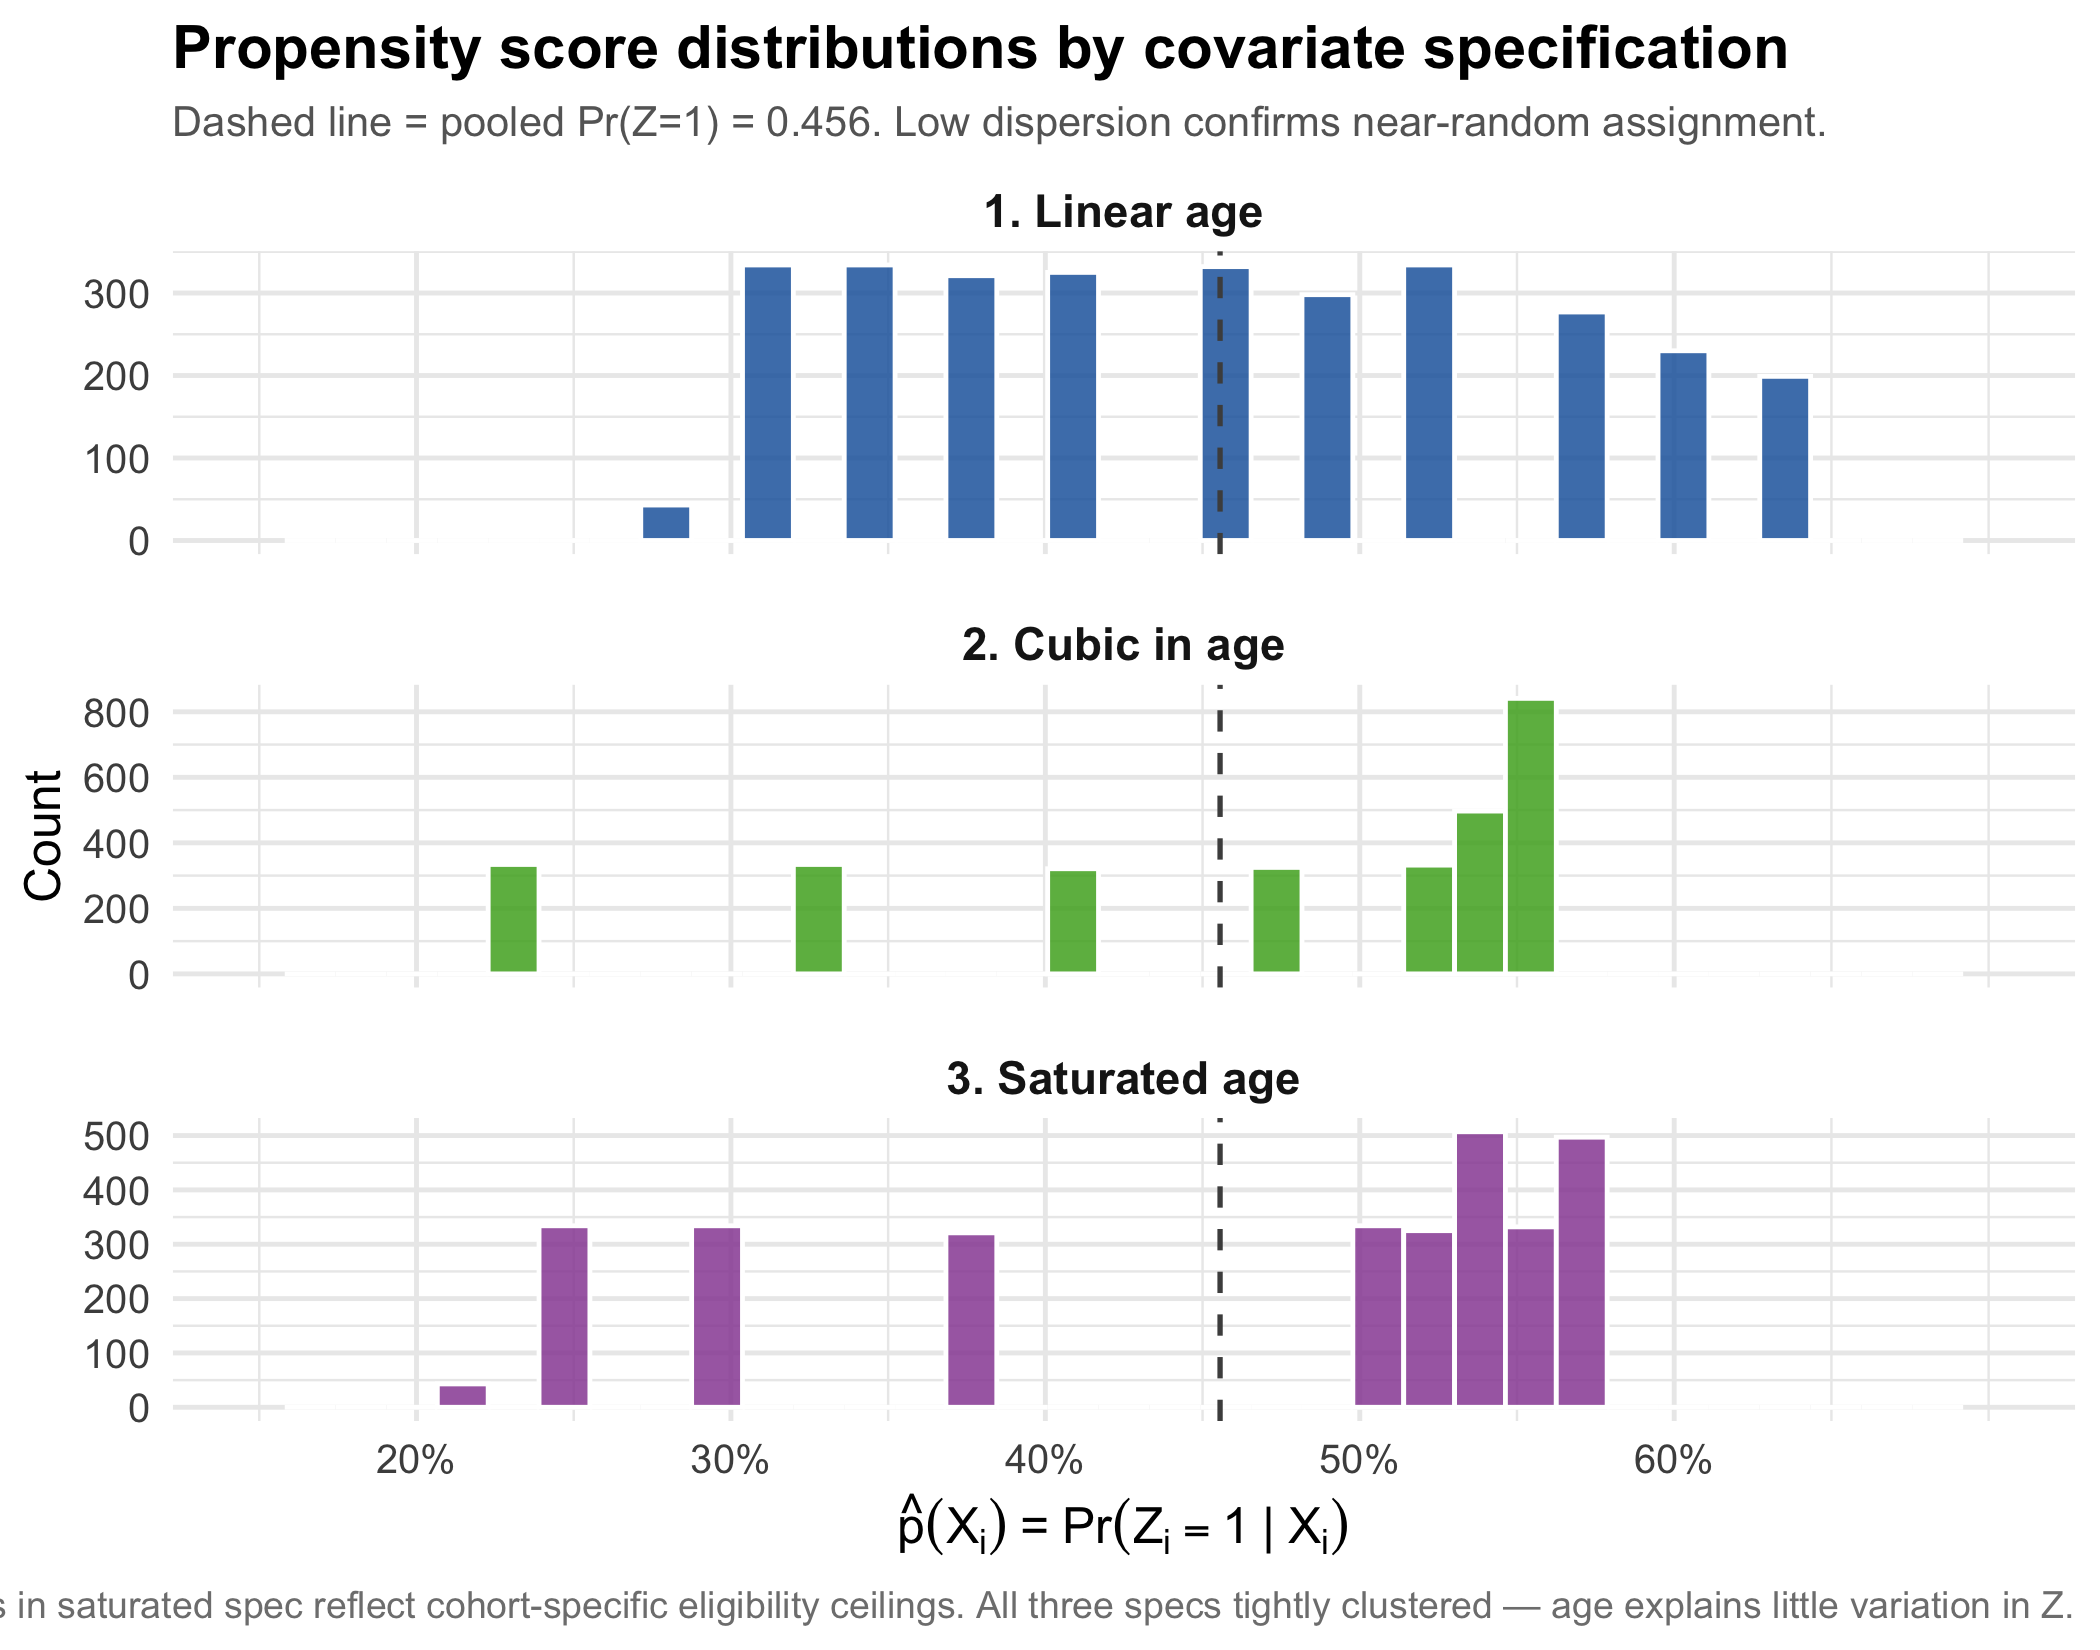
\includegraphics[width=0.85\textwidth]{pics/i_pscore.png}
\caption{The first Empirical Application : Distribution of the fitted propensity score
  $\hat{p}(X_i) = \Pr(Z_i=1 \mid X_i)$ under three covariate
  specifications.}
\label{fig:vietnam_pscore}
\end{figure}

\subsection{Vietnam Design diagnostics}
\begin{table}[H]
\centering
\caption{Design diagnostics: Vietnam draft lottery}
\label{tab:vietnam_descr}
\begin{threeparttable}
\begin{tabular}{@{}lcc@{}}
\toprule
Quantity or specification & Estimate & Robust \(t^2\) \\
\midrule
Sample size \(N\)                              & \(3{,}027\) &  \\
\(P(Z_i=1)\)                                   & \(0.456\)   &  \\
\(P(D_i=1\mid Z_i=0)\)                         & \(0.265\)   &  \\
\(P(D_i=1\mid Z_i=1)\)                         & \(0.404\)   &  \\
Unadjusted uptake difference                   & \(0.139\)   &  \\
\addlinespace
First stage, linear age                        & \(0.0949\)  & \(30.1\) \\
First stage, cubic age                         & \(0.0882\)  & \(26.3\) \\
First stage, saturated age                     & \(0.0899\)  & \(27.2\) \\
\bottomrule
\end{tabular}
\begin{tablenotes}
\footnotesize
\item Robust \(t^2\) is the squared HC1-robust \(t\)-statistic for the excluded
instrument.
\end{tablenotes}
\end{threeparttable}
\end{table}


\subsection{Estimates kappa vs dml}

\begin{table}[H]
\centering
\caption{Point estimates for log hourly wages across age specifications}
\label{tab:vietnam_point_estimates_age}
\small
\begin{threeparttable}
\begin{tabular}{@{}lccc@{}}
\toprule
Estimator
& Linear age
& Cubic age
& Saturated age \\
\midrule

\multicolumn{4}{l}{\textit{Panel A: 2SLS benchmark}} \\[2pt]

2SLS
& 0.233\,(0.212)
& 0.227\,(0.229)
& 0.254\,(0.227) \\[4pt]

\multicolumn{4}{l}{\textit{Panel B: Normalised kappa estimators}} \\[2pt]

$\hat{\tau}_{u}^{cb}$
& 0.229\,(0.213)
& 0.210\,(0.233)
& 0.241\,(0.229) \\

$\hat{\tau}_{u}^{ml}$
& 0.234\,(0.211)
& 0.202\,(0.235)
& 0.241\,(0.229) \\

$\hat{\tau}_{a,10}$
& 0.227\,(0.204)
& 0.204\,(0.239)
& 0.241\,(0.229) \\[4pt]

\multicolumn{4}{l}{\textit{Panel C: Unnormalised kappa estimators}} \\[2pt]

$\hat{\tau}_{a}$
& 0.015\,(0.207)
& 0.314\,(0.252)
& 0.241\,(0.229) \\

$\hat{\tau}_{t}$
& 0.016\,(0.219)
& 0.302\,(0.240)
& 0.241\,(0.229) \\

$\hat{\tau}_{a,0}$
& 0.014\,(0.199)
& 0.317\,(0.255)
& 0.241\,(0.229) \\[4pt]

\multicolumn{4}{l}{\textit{Panel D: DML with honest-forest nuisances}} \\[2pt]

PLR-IV
& n.a.
& 0.243\,(0.228)
& 0.242\,(0.228) \\

Wald-AIPW
& n.a.
& 0.229\,(0.231)
& 0.244\,(0.233) \\

\bottomrule
\end{tabular}

\begin{tablenotes}
\footnotesize
\item \textit{Notes:} The outcome is log hourly wages measured in
dollars. The 2SLS and kappa results correspond to the dollar specifications
in the replication of Table~2 in \citet{sloczynski2025abadie}. The DML
nuisance functions are estimated using tuned honest forests with five-fold
cross-fitting.  
\end{tablenotes}
\end{threeparttable}
\end{table}





\subsection{Estimates flexible nuisance}
\begin{table}[H]
\centering
\caption{DML point estimates across nuisance learners}
\label{tab:vietnam_dml_learners}
\small
\begin{threeparttable}
\begin{tabular}{@{}lcccc@{}}
\toprule
& \multicolumn{2}{c}{PLR-IV}
& \multicolumn{2}{c}{Wald-AIPW} \\
\cmidrule(lr){2-3}
\cmidrule(lr){4-5}
Nuisance learner
& Cubic age
& Saturated age
& Cubic age
& Saturated age \\
\midrule

Honest forest
& 0.243\,(0.228)
& 0.242\,(0.228)
& 0.229\,(0.231)
& 0.244\,(0.233) \\

Regression
& 0.239\,(0.231)
& 0.270\,(0.230)
& 0.218\,(0.233)
& 0.247\,(0.234) \\

Random forest
& 0.270\,(0.230)
& 0.283\,(0.223)
& 0.246\,(0.234)
& 0.261\,(0.224) \\

XGBoost
& 0.265\,(0.229)
& 0.281\,(0.230)
& 0.238\,(0.228)
& 0.253\,(0.230) \\

\bottomrule
\end{tabular}

\begin{tablenotes}
\footnotesize
\item \textit{Notes:} The outcome is log hourly wages measured in
dollars. All specifications use five-fold cross-fitting. 
\end{tablenotes}
\end{threeparttable}
\end{table}


\subsection{Numerical difference in the cubic CBPS replication}
\label{subsubsec:vietnam_cbps_replication}

The only difference from the published table is the cubic-age
\(\hat{\tau}_{u}^{cb}\) estimate. Both implementations use the same sample,
covariates, estimator, and sandwich variance formula. The difference arises
from the numerical solution of the CBPS balancing conditions in a poorly
conditioned cubic polynomial. The Stata solution underlying the published
value has a maximum absolute balancing residual of
\(5.45\times10^{-4}\), whereas the standardised R solver reduces this
residual to \(4.41\times10^{-14}\). Supplying the Stata propensity scores to
the R estimator reproduces both the published estimate and its standard
error. 









\clearpage
\begin{sidewaystable}[p]
\raggedright
\subsection{Vietnam Outcome-Weight Diagnostics}
\centering
\caption{Complete eligible outcome-weight diagnostics for the Vietnam application}
\label{tab:vietnam_weights_full_appendix}
\footnotesize
\setlength{\tabcolsep}{5pt}
\renewcommand{\arraystretch}{0.95}
\begin{threeparttable}
\begin{tabular}{@{}l r c c c r@{}}
\toprule
Estimator
& $\sum_i\omega_i$
& Mass T/C
& $\mathrm{ESS}_{\mathrm{mod}}/N$ T/C
& Opposite-sign mass T/C (\%)
& $\max_i|\omega_i|$ \\
\midrule
\multicolumn{6}{l}{\textit{Panel A: Cubic age specification}} \\[1pt]
PLR-IV, tuned forest
& 0.000000 & 0.994/0.994
& 0.963/0.921 & 43.5/46.6 & 0.012494 \\
Wald-AIPW, tuned forest
& 0.000000 & 1.000/1.000
& 0.952/0.910 & 43.4/46.7 & 0.017627 \\
Wald-AIPW, OLS/logit
& 0.000000 & 0.991/0.991
& 0.955/0.908 & 43.5/46.8 & 0.026926 \\
PLR-IV, \texttt{ranger}
& 0.000000 & 0.999/0.999
& 0.960/0.916 & 43.5/46.6 & 0.013538 \\
Wald-AIPW, \texttt{ranger}
& 0.000000 & 0.999/0.999
& 0.948/0.903 & 43.4/46.7 & 0.021647 \\[1pt]
$\hat{\tau}_{u}^{cb}$
& 0.000000 & 1.000/1.000
& 0.958/0.908 & 43.5/46.8 & 0.025384 \\
$\hat{\tau}_{u}^{ml}$
& 0.000000 & 1.000/1.000
& 0.954/0.899 & 43.6/46.8 & 0.028108 \\
$\hat{\tau}_{a,10}$
& 0.000000 & 1.000/1.000
& 0.954/0.898 & 43.5/46.9 & 0.029078 \\
$\hat{\tau}_{a}$
& 0.048243 & 1.041/0.993
& 0.954/0.898 & 43.5/46.9 & 0.028869 \\
$\hat{\tau}_{t}$
& 0.046342 & 1.000/0.954
& 0.954/0.898 & 43.5/46.9 & 0.027731 \\
$\hat{\tau}_{a,0}$
& 0.048594 & 1.049/1.000
& 0.954/0.898 & 43.5/46.9 & 0.029078 \\[3pt]
\multicolumn{6}{l}{\textit{Panel B: Saturated age specification}} \\[1pt]
PLR-IV, tuned forest
& 0.000000 & 0.999/0.999
& 0.961/0.917 & 43.5/46.6 & 0.013128 \\
Wald-AIPW, tuned forest
& 0.000000 & 1.005/1.005
& 0.951/0.908 & 43.4/46.7 & 0.016866 \\
PLR-IV, OLS
& 0.000000 & 1.000/1.000
& 0.960/0.916 & 43.5/46.6 & 0.013426 \\
Wald-AIPW, OLS/logit
& 0.000000 & 1.000/1.000
& 0.948/0.903 & 43.4/46.7 & 0.021773 \\
PLR-IV, \texttt{ranger}
& 0.000000 & 1.003/1.003
& 0.964/0.924 & 43.3/46.5 & 0.011886 \\
Wald-AIPW, \texttt{ranger}
& 0.000000 & 1.005/1.005
& 0.951/0.914 & 43.1/46.6 & 0.016211 \\[1pt]
$\hat{\tau}_{u}^{cb}$
& 0.000000 & 1.000/1.000
& 0.953/0.909 & 43.3/46.7 & 0.017811 \\
$\hat{\tau}_{u}^{ml}$
& 0.000000 & 1.000/1.000
& 0.953/0.909 & 43.3/46.7 & 0.017811 \\
$\hat{\tau}_{a,10}$
& 0.000000 & 1.000/1.000
& 0.953/0.909 & 43.3/46.7 & 0.017811 \\
$\hat{\tau}_{a}$
& 0.000000 & 1.000/1.000
& 0.953/0.909 & 43.3/46.7 & 0.017811 \\
$\hat{\tau}_{t}$
& 0.000000 & 1.000/1.000
& 0.953/0.909 & 43.3/46.7 & 0.017811 \\
$\hat{\tau}_{a,0}$
& 0.000000 & 1.000/1.000
& 0.953/0.909 & 43.3/46.7 & 0.017811 \\
\bottomrule
\end{tabular}
\begin{tablenotes}
\footnotesize
\item \textit{Notes:} T/C denotes treated and sign-oriented control values.
Mass T/C reports the treated weight mass and the sign-oriented control mass.
Modified ESS is divided by the observed number of treated or control
observations. Only algebraic weights or reconstructed vectors that reproduce
their estimator under the estimator-specific \texttt{all.equal()} check are
included. The forest rows use the tuned specifications.
\end{tablenotes}
\end{threeparttable}
\end{sidewaystable}

\clearpage
\begin{table}[H]
\centering
\caption{Outcome-weight representation audit for excluded Vietnam vectors}
\label{tab:vietnam_weight_representation_audit}
\footnotesize
\begin{threeparttable}
\begin{tabular}{@{}l l r c@{}}
\toprule
Estimator
& Age specification
& $|\omega'Y-\hat{\tau}|$
& \(\omega'Y\) reproduces \(\hat{\tau}\) \\
\midrule
PLR-IV, OLS
& Cubic & $3.71\times10^{-9}$ & FALSE \\
PLR-IV, tuned XGBoost
& Cubic & $1.18\times10^{-7}$ & FALSE \\
Wald-AIPW, tuned XGBoost
& Cubic & $3.99\times10^{-9}$ & FALSE \\
PLR-IV, tuned XGBoost
& Saturated & $1.17\times10^{-7}$ & FALSE \\
Wald-AIPW, tuned XGBoost
& Saturated & $3.46\times10^{-8}$ & FALSE \\
\bottomrule
\end{tabular}
\begin{tablenotes}
\footnotesize
\item \textit{Notes:} Each fitted estimator is assessed separately using
Knaus's \texttt{all.equal()} criterion with R's default tolerance. These
vectors remain in the point-estimate analysis but are excluded from
normalisation, concentration, and balance diagnostics. The cubic OLS
PLR-IV result is a borderline numerical-conditioning artefact: a QR-based
reconstruction matching \texttt{lm} reduces the gap to
\(3.34\times10^{-13}\) and returns TRUE, but that alternative reconstruction
is not used in the reported diagnostics.
\end{tablenotes}
\end{threeparttable}
\end{table}

\clearpage
\subsection{Vietnam Covariate-Balance Diagnostics}
\begin{figure}[H]
\centering
\includegraphics[width=\textwidth]{pics/vietnam_love_cubic_thesis.png}
\caption{Covariate balance under cubic age adjustment}
\label{fig:vietnam_love_cubic}
\begin{minipage}{0.96\textwidth}
\footnotesize
\textit{Notes:} Dark circles report the unadjusted absolute standardised mean
differences. Yellow triangles report the differences after applying the
estimator-specific outcome weights. The dashed vertical line marks \(0.1\).
The XGBoost panels use the reconstructed tuned weight vectors. Balance is
calculated with \texttt{cobalt} \citep{greifer2024cobalt}.
\end{minipage}
\end{figure}

\begin{figure}[H]
\centering
\includegraphics[width=\textwidth]{pics/vietnam_love_saturated_thesis.png}
\caption{Covariate balance under saturated age adjustment}
\label{fig:vietnam_love_saturated}
\begin{minipage}{0.96\textwidth}
\footnotesize
\textit{Notes:} Dark circles report the unadjusted absolute differences in
the binary age indicators. Yellow triangles report the differences after
applying the estimator-specific outcome weights. The dashed vertical line
marks \(0.1\). The XGBoost panels use the reconstructed tuned weight vectors.
Balance is calculated with \texttt{cobalt} \citep{greifer2024cobalt}.
\end{minipage}
\end{figure}

% Here is where I start the Card application 



\clearpage

\section{Card Application: Additional Results and Diagnostics}
\label{app:card_design_diagnostics}

\subsection{Variables and Covariate Specifications}
\label{app:card_variables}

\begin{table}[H]
\centering
\caption{Instrument, treatments, and outcome in the Card application}
\label{tab:card_design_appendix}
\small
\begin{tabular}{lll}
\toprule
Role & Symbol & Definition \\
\midrule
Instrument & $Z_i$ & Grew up near a four-year college in 1966 \\
Treatment 1 & $D_{1i}$ & Schooling beyond high school,
\(\mathbf{1}\{\texttt{educ}_i>12\}\) \\
Treatment 2 & $D_{2i}$ & At least sixteen years of schooling,
\(\mathbf{1}\{\texttt{educ}_i\geq16\}\) \\
Outcome & $Y_i$ & Log hourly wage \\
\bottomrule
\end{tabular}
\end{table}

\begin{table}[H]
\centering
\caption{Covariate specifications in the Card application}
\label{tab:card_covariates_appendix}
\small
\begin{tabular}{lcc}
\toprule
Covariate & Card specification & Kitagawa specification \\
\midrule
Experience and experience squared & Yes & No \\
Black indicator & Yes & Yes \\
Southern residence in 1976 & Yes & Yes \\
Metropolitan residence in 1976 & Yes & Yes \\
Metropolitan residence in 1966 & Yes & Yes \\
Southern residence in 1966 & No & Yes \\
Regional indicators, \texttt{reg661}, \(\ldots\), \texttt{reg668} & Yes & No \\
\bottomrule
\end{tabular}
\end{table}

\subsection{Card Descriptive diagnostics}
\label{app:card_propensity}



\begin{table}[H]
\centering
\caption{First-stage, linear-IV, and instrument-propensity diagnostics}
\label{tab:card_descriptive_diagnostics}
\scriptsize
\begin{threeparttable}

\textit{Panel A: Treatment rates and linear-IV building blocks}\\[2pt]
\setlength{\tabcolsep}{3.5pt}
\begin{tabular}{llrrrrrr}
\toprule
Treatment & Specification
& \(\Pr(D=1\mid Z=0)\)
& \(\Pr(D=1\mid Z=1)\)
& \shortstack{Adjusted first stage\\(HC1 SE)}
& Robust \(t^2\)
& \shortstack{Adjusted\\Wald}
& \shortstack{Raw\\Wald} \\
\midrule
\texttt{somecol} & Card
& 0.422 & 0.544 & 0.0636 (0.0180) & 12.5 & 0.6613 & 1.2787 \\
\texttt{somecol} & Kitagawa
& 0.422 & 0.544 & 0.0653 (0.0218) & 9.0 & 0.5748 & 1.2787 \\
\texttt{educ16} & Card
& 0.225 & 0.293 & 0.0302 (0.0162) & 3.5 & 1.3915 & 2.2737 \\
\texttt{educ16} & Kitagawa
& 0.225 & 0.293 & 0.0379 (0.0191) & 3.9 & 0.9909 & 2.2737 \\
\bottomrule
\end{tabular}

\vspace{0.8em}
\textit{Panel B: Fitted instrument-propensity support}\\[2pt]
\setlength{\tabcolsep}{5pt}
\begin{tabular}{lrrrrrr}
\toprule
Specification & Fitted range & SD & Max., \(Z=0\)
& \shortstack{\(Z=0\)\\\(\hat p>.90\)}
& Min., \(Z=1\)
& \shortstack{\(Z=1\)\\\(\hat p<.10\)} \\
\midrule
Card
& \([0.1724,0.9517]\) & 0.2356 & 0.9357 & 40 & 0.1724 & 0 \\
Kitagawa
& \([0.2532,0.9067]\) & 0.2280 & 0.9067 & 9 & 0.2532 & 0 \\
\bottomrule
\end{tabular}

\begin{tablenotes}
\footnotesize
\item \textit{Notes:} The sample contains \(957\) observations with \(Z=0\)
and \(2{,}053\) with \(Z=1\). The adjusted first stage is obtained from a
linear probability model using the stated conditioning set. Robust \(t^2\) is
the squared HC1-robust \(t\)-statistic for \(Z_i\). The adjusted Wald ratio uses
the covariate-adjusted reduced form and first stage; the raw Wald ratio uses
unconditional group-mean differences. The outcome is log hourly wage.
\end{tablenotes}
\end{threeparttable}
\end{table}




\subsection{Instrument-Propensity Support}
\label{app:card_propensity_support}

\begin{figure}[H]
\centering
\includegraphics[width=0.92\textwidth]{pics/card_propensity_support.png}
\caption{Distribution of the fitted instrument propensity score by instrument status}
\label{fig:card_propensity_appendix}
\begin{minipage}{0.92\textwidth}
\footnotesize
\textit{Notes:} The panels show the Card and Kitagawa conditioning sets,
separately for observations with \(Z=1\) and \(Z=0\). The dashed line marks
the pooled instrument share. The figure describes empirical support and is
not a test of the IV assumptions.
\end{minipage}
\end{figure}












\subsection{Point Estimates and Learner Tuning}
\label{app:card_point_estimates}

\begin{figure}[H]
\centering
\includegraphics[width=\textwidth]{pics/card_point_estimates_selected.png}
\caption{Selected estimates across treatment margins and conditioning sets}
\label{fig:card_point_estimates_appendix}
\begin{minipage}{0.96\textwidth}
\footnotesize
\textit{Notes:} Points report estimates of the effect on log hourly wage and
lines report \(95\%\) confidence intervals. The Card and Kitagawa
specifications use different conditioning sets. The XGBoost and honest-forest
rows use tuned nuisance models. Untuned XGBoost is excluded because its
extreme estimates would make the remaining comparisons unreadable; the
untuned and tuned results are reported in
Table~\ref{tab:card_xgb_tuning_appendix}.
\end{minipage}
\end{figure}

\begin{table}[H]
\centering
\caption{Selected point estimates in the Card application}
\label{tab:card_selected_estimates_appendix}
\scriptsize
\setlength{\tabcolsep}{4pt}
\begin{threeparttable}
\begin{tabular}{lcccc}
\toprule
& \multicolumn{2}{c}{Schooling beyond high school}
& \multicolumn{2}{c}{At least sixteen years} \\
\cmidrule(lr){2-3}\cmidrule(lr){4-5}
Estimator & Card & Kitagawa & Card & Kitagawa \\
\midrule
2SLS
& 0.661 (0.295) & 0.575 (0.308)
& 1.392 (0.801) & 0.991 (0.611) \\
\addlinespace
\(\hat{\tau}^{cb}_{u}\)
& 0.376 (0.223) & 0.331 (0.236)
& 0.853 (0.549) & 0.588 (0.433) \\
\(\hat{\tau}^{ml}_{u}\)
& 0.331 (0.202) & 0.356 (0.244)
& 0.619 (0.387) & 0.628 (0.448) \\
\(\hat{\tau}^{ml}_{t}\)
& 0.171 (0.367) & 0.769 (0.308)
& 0.319 (0.687) & 1.367 (0.648) \\
\addlinespace
PLR-IV, tuned forest
& 0.681 (0.289) & 0.593 (0.340)
& 1.140 (0.535) & 1.030 (0.684) \\
Wald-AIPW, tuned forest
& 0.279 (0.214) & 0.292 (0.249)
& 0.530 (0.398) & 0.535 (0.462) \\
PLR-IV, tuned XGBoost
& 0.577 (0.258) & 0.612 (0.350)
& 0.956 (0.459) & 1.010 (0.655) \\
Wald-AIPW, tuned XGBoost
& 0.382 (0.214) & 0.238 (0.258)
& 0.730 (0.429) & 0.477 (0.514) \\
\bottomrule
\end{tabular}
\begin{tablenotes}
\footnotesize
\item \textit{Notes:} Each cell reports the point estimate followed by its
standard error in parentheses. The outcome is log hourly wage measured in
dollars. The 2SLS and kappa rows reproduce the corresponding results in
\citet[Table~3]{sloczynski2025abadie}. DML estimates use five-fold
cross-fitting. Hyperparameter tuning is based only on nuisance-prediction
loss.
\end{tablenotes}
\end{threeparttable}
\end{table}



\begin{table}[H]
\centering
\caption{Nested XGBoost tuning for Wald-AIPW}
\label{tab:card_xgb_tuning_appendix}
\scriptsize
\setlength{\tabcolsep}{5pt}
\begin{threeparttable}
\begin{tabular}{@{}lccc@{}}
\toprule
Design cell
& \shortstack{Untuned\\estimate (SE)}
& \shortstack{Tuned\\estimate (SE)}
& \shortstack{Boundary share\\untuned \(\rightarrow\) tuned} \\
\midrule
Card--schooling beyond high school
& \(-13.416\) (14.411) & 0.382 (0.214)
& \(0.3453\rightarrow0.1312\) \\
Card--at least sixteen years
& \(-3.198\) (4.054) & 0.730 (0.429)
& \(0.3759\rightarrow0.1106\) \\
Kitagawa--schooling beyond high school
& \(-0.113\) (0.627) & 0.238 (0.258)
& \(0.0045\rightarrow0.0000\) \\
Kitagawa--at least sixteen years
& \(-3.656\) (100.914) & 0.477 (0.514)
& \(0.0053\rightarrow0.0002\) \\
\bottomrule
\end{tabular}
\begin{tablenotes}
\footnotesize
\item \textit{Notes:} Hyperparameters are selected separately within each
outer training fold using nuisance-prediction loss. The treatment-effect
estimate is not used for tuning. Boundary share is the fraction of fitted
instrument or treatment propensities below \(0.02\) or above \(0.98\).
\end{tablenotes}
\end{threeparttable}
\end{table}






\subsection{Complete-Pipeline Translation-Invariance Results}
\label{app:card_translation}


\begin{table}[H]
\centering
\caption{Complete kappa translation-invariance results in the Card application}
\label{tab:card_translation_kappa_appendix}
\footnotesize
\setlength{\tabcolsep}{4pt}
\begin{threeparttable}
\begin{tabular}{@{}lrrr rrr@{}}
\toprule
& \multicolumn{3}{c}{Schooling beyond high school}
& \multicolumn{3}{c}{At least 16 years} \\
\cmidrule(lr){2-4}\cmidrule(lr){5-7}
Estimator
& Dollars & Cents & Change
& Dollars & Cents & Change \\
\midrule
\multicolumn{7}{l}{\textit{Panel A: Card conditioning set}} \\[2pt]
$\hat{\tau}^{cb}_{u}$
& 0.376202 & 0.376202 & 0.000000
& 0.853043 & 0.853043 & 0.000000 \\
$\hat{\tau}^{ml}_{u}$
& 0.330794 & 0.330794 & 0.000000
& 0.619076 & 0.619076 & 0.000000 \\
$\hat{\tau}^{ml}_{a,10}$
& 0.345951 & 0.345951 & 0.000000
& 0.586239 & 0.586239 & 0.000000 \\
\addlinespace
$\hat{\tau}^{ml}_{a}$
& 0.169541 & $-0.319298$ & \textbf{$-0.488839$}
& 0.315357 & $-0.593916$ & \textbf{$-0.909273$} \\
$\hat{\tau}^{ml}_{t}$
& 0.170674 & $-0.321432$ & \textbf{$-0.492106$}
& 0.319300 & $-0.601342$ & \textbf{$-0.920642$} \\
$\hat{\tau}^{ml}_{a,0}$
& 0.154196 & $-0.290400$ & \textbf{$-0.444597$}
& 0.266102 & $-0.501154$ & \textbf{$-0.767256$} \\
\addlinespace[4pt]
\multicolumn{7}{l}{\textit{Panel B: Kitagawa conditioning set}} \\[2pt]
$\hat{\tau}^{cb}_{u}$
& 0.330974 & 0.330974 & 0.000000
& 0.588471 & 0.588471 & 0.000000 \\
$\hat{\tau}^{ml}_{u}$
& 0.355581 & 0.355581 & 0.000000
& 0.627555 & 0.627555 & 0.000000 \\
$\hat{\tau}^{ml}_{a,10}$
& 0.293036 & 0.293036 & 0.000000
& 0.835610 & 0.835610 & 0.000000 \\
\addlinespace
$\hat{\tau}^{ml}_{a}$
& 0.841801 & 2.247603 & \textbf{1.405803}
& 1.616829 & 4.316925 & \textbf{2.700096} \\
$\hat{\tau}^{ml}_{t}$
& 0.768756 & 2.052575 & \textbf{1.283819}
& 1.367301 & 3.650688 & \textbf{2.283386} \\
$\hat{\tau}^{ml}_{a,0}$
& 1.065907 & 2.845967 & \textbf{1.780059}
& 2.711990 & 7.240998 & \textbf{4.529008} \\
\bottomrule
\end{tabular}
\begin{tablenotes}
\footnotesize
\item \textit{Notes:} ``Change'' is the cent-recoded estimate minus the
dollar estimate. The first three estimators in each panel are normalised and
the final three are unnormalised. Bold changes exceed \(10^{-4}\) in
absolute value.
\end{tablenotes}
\end{threeparttable}
\end{table}




\begin{table}[H]
\centering
\caption{Complete DML translation-invariance results in the Card application}
\label{tab:card_translation_dml_appendix}
\scriptsize
\setlength{\tabcolsep}{3.3pt}
\begin{threeparttable}
\begin{tabular}{@{}lrrr rrr@{}}
\toprule
& \multicolumn{3}{c}{Schooling beyond high school}
& \multicolumn{3}{c}{At least 16 years} \\
\cmidrule(lr){2-4}\cmidrule(lr){5-7}
Estimator
& Dollars & Cents & Change
& Dollars & Cents & Change \\
\midrule
\multicolumn{7}{l}{\textit{Panel A: Card conditioning set}} \\[2pt]
PLR-IV, tuned honest forest
& 0.680717 & 0.680161 & \textbf{$-0.000556$}
& 1.139922 & 1.138991 & \textbf{$-0.000931$} \\
Wald-AIPW, tuned honest forest
& 0.279284 & 0.277579 & \textbf{$-0.001706$}
& 0.530289 & 0.527051 & \textbf{$-0.003239$} \\
\addlinespace
PLR-IV, linear
& 0.677860 & 0.677860 & 0.000000
& 1.418913 & 1.418913 & 0.000000 \\
Wald-AIPW, linear/logit
& 0.399125 & 0.399125 & 0.000000
& 0.884278 & 0.884278 & 0.000000 \\
\addlinespace
PLR-IV, \texttt{ranger}
& 0.685262 & 0.684654 & \textbf{$-0.000608$}
& 1.112339 & 1.111352 & \textbf{$-0.000987$} \\
Wald-AIPW, \texttt{ranger}
& 0.262065 & 0.261714 & \textbf{$-0.000351$}
& 0.492577 & 0.491918 & \textbf{$-0.000659$} \\
\addlinespace
PLR-IV, tuned XGBoost
& 0.577421 & 0.564233 & \textbf{$-0.013188$}
& 0.955600 & 0.933774 & \textbf{$-0.021826$} \\
Wald-AIPW, tuned XGBoost
& 0.382135 & 0.381906 & \textbf{$-0.000229$}
& 0.729903 & 0.729465 & \textbf{$-0.000438$} \\
\addlinespace[4pt]
\multicolumn{7}{l}{\textit{Panel B: Kitagawa conditioning set}} \\[2pt]
PLR-IV, tuned honest forest
& 0.592544 & 0.592558 & 0.000014
& 1.030285 & 1.030310 & 0.000025 \\
Wald-AIPW, tuned honest forest
& 0.292078 & 0.292128 & 0.000050
& 0.534740 & 0.534831 & 0.000091 \\
\addlinespace
PLR-IV, linear
& 0.567899 & 0.567899 & 0.000000
& 0.942714 & 0.942714 & 0.000000 \\
Wald-AIPW, linear/logit
& 0.311215 & 0.311215 & 0.000000
& 0.533596 & 0.533596 & 0.000000 \\
\addlinespace
PLR-IV, \texttt{ranger}
& 0.622533 & 0.622542 & 0.000010
& 1.044640 & 1.044657 & 0.000017 \\
Wald-AIPW, \texttt{ranger}
& 0.294268 & 0.294271 & 0.000003
& 0.514201 & 0.514206 & 0.000005 \\
\addlinespace
PLR-IV, tuned XGBoost
& 0.611863 & 0.612182 & \textbf{0.000319}
& 1.010447 & 1.010973 & \textbf{0.000527} \\
Wald-AIPW, tuned XGBoost
& 0.238095 & 0.242311 & \textbf{0.004216}
& 0.476512 & 0.484949 & \textbf{0.008437} \\
\bottomrule
\end{tabular}
\begin{tablenotes}
\scriptsize
\item \textit{Notes:} ``Change'' is the cent-recoded estimate minus the
dollar estimate after repeating the complete estimation procedure. XGBoost
uses fold-specific nested tuning under the same search design for both
outcome codings. Bold changes exceed \(10^{-4}\) in absolute value.
\end{tablenotes}
\end{threeparttable}
\end{table}


\subsection{Outcome-Weight Normalisation and Concentration}
\label{app:card_weights}

\begin{table}[H]
\centering
\caption{Selected outcome-weight diagnostics in the Card application}
\label{tab:card_weight_diagnostics_appendix}
\scriptsize
\setlength{\tabcolsep}{4pt}
\begin{tabular}{llrrr}
\toprule
Cell & Estimator & \shortstack{Treated/control\\mass} &
\(ESS_{\mathrm{mod}}\) & \(\max_i|\omega_i|\) \\
\midrule
Card, \(D_1\) & PLR-IV, tuned forest & 1.00/1.00 & 1819 & 0.033 \\
 & Wald-AIPW, tuned forest & 0.97/0.97 & 1345 & 0.146 \\
 & $\hat{\tau}^{ml}_{u}$ & 1.00/1.00 & 1569 & 0.052 \\
 & $\hat{\tau}^{ml}_{t}$ & 1.00/1.11 & 1561 & 0.055 \\
\addlinespace
Card, \(D_2\) & PLR-IV, tuned forest & 0.96/0.96 & 1819 & 0.055 \\
 & Wald-AIPW, tuned forest & 0.94/0.94 & 1345 & 0.277 \\
 & $\hat{\tau}^{ml}_{u}$ & 1.00/1.00 & 1569 & 0.097 \\
 & $\hat{\tau}^{ml}_{t}$ & 1.00/1.20 & 1561 & 0.103 \\
\addlinespace
Kitagawa, \(D_1\) & PLR-IV, tuned forest & 1.00/1.00 & 1954 & 0.033 \\
 & Wald-AIPW, tuned forest & 0.99/0.99 & 1631 & 0.065 \\
 & $\hat{\tau}^{ml}_{u}$ & 1.00/1.00 & 1764 & 0.038 \\
 & $\hat{\tau}^{ml}_{t}$ & 1.00/0.72 & 1786 & 0.038 \\
\addlinespace
Kitagawa, \(D_2\) & PLR-IV, tuned forest & 1.01/1.01 & 1954 & 0.057 \\
 & Wald-AIPW, tuned forest & 1.01/1.01 & 1631 & 0.119 \\
 & $\hat{\tau}^{ml}_{u}$ & 1.00/1.00 & 1764 & 0.078 \\
 & $\hat{\tau}^{ml}_{t}$ & 1.00/0.50 & 1786 & 0.067 \\
\bottomrule
\end{tabular}
\begin{minipage}{0.96\textwidth}
\footnotesize
\textit{Notes:} Control mass is the negative of the sum of control-group
weights, so a fully normalised treated-minus-control comparison has mass
\(1/1\). Modified effective sample size is used because the outcome weights
are signed. The table reports selected estimators needed to interpret the
translation result.
\end{minipage}
\end{table}



\clearpage
\subsection{Complete Outcome-Weight Diagnostics}
\label{app:card_weights_complete}

Tables~\ref{tab:card_kappa_weights_appendix}
and~\ref{tab:card_dml_weights_appendix} report all eligible outcome-weight
diagnostics. The tables retain the four design cells as separate panels to
avoid mixing the two treatment definitions or conditioning sets.

\begin{table}[H]
\centering
\caption{Complete kappa outcome-weight diagnostics in the Card application}
\label{tab:card_kappa_weights_appendix}
\scriptsize
\setlength{\tabcolsep}{3.6pt}
\begin{threeparttable}
\begin{tabular}{@{}lrrrrr@{}}
\toprule
Estimator
& \(\sum_i\omega_i\)
& Mass T/C
& \shortstack{Opposite-sign\\mass T/C (\%)}
& \shortstack{$\mathrm{ESS}_{\mathrm{mod}}/N$\\T/C}
& \(\max_i|\omega_i|\) \\
\midrule
\multicolumn{6}{l}{\textit{Panel A: Card, schooling beyond high school}} \\[2pt]
$\hat{\tau}^{cb}_{u}$    & 0.000000 & 1.000 / 1.000 & 45.5 / 46.0 & 0.575 / 0.510 & 0.086905 \\
$\hat{\tau}^{ml}_{u}$    & 0.000000 & 1.000 / 1.000 & 44.8 / 45.3 & 0.561 / 0.497 & 0.051920 \\
$\hat{\tau}^{ml}_{a,10}$ & 0.000000 & 1.000 / 1.000 & 45.0 / 45.1 & 0.558 / 0.495 & 0.054816 \\
$\hat{\tau}^{ml}_{a}$    & $-0.106150$ & 0.993 / 1.100 & 45.0 / 45.1 & 0.558 / 0.495 & 0.054452 \\
$\hat{\tau}^{ml}_{t}$    & $-0.106860$ & 1.000 / 1.107 & 45.0 / 45.1 & 0.558 / 0.495 & 0.054816 \\
$\hat{\tau}^{ml}_{a,0}$  & $-0.096543$ & 0.903 / 1.000 & 45.0 / 45.1 & 0.558 / 0.495 & 0.049524 \\
\addlinespace[4pt]
\multicolumn{6}{l}{\textit{Panel B: Card, at least 16 years}} \\[2pt]
$\hat{\tau}^{cb}_{u}$    & 0.000000 & 1.000 / 1.000 & 46.3 / 48.7 & 0.571 / 0.525 & 0.197058 \\
$\hat{\tau}^{ml}_{u}$    & 0.000000 & 1.000 / 1.000 & 44.7 / 48.2 & 0.577 / 0.508 & 0.097168 \\
$\hat{\tau}^{ml}_{a,10}$ & 0.000000 & 1.000 / 1.000 & 45.0 / 48.0 & 0.574 / 0.505 & 0.102551 \\
$\hat{\tau}^{ml}_{a}$    & $-0.197446$ & 0.988 / 1.185 & 45.0 / 48.0 & 0.574 / 0.505 & 0.101285 \\
$\hat{\tau}^{ml}_{t}$    & $-0.199915$ & 1.000 / 1.200 & 45.0 / 48.0 & 0.574 / 0.505 & 0.102551 \\
$\hat{\tau}^{ml}_{a,0}$  & $-0.166608$ & 0.833 / 1.000 & 45.0 / 48.0 & 0.574 / 0.505 & 0.085466 \\
\addlinespace[4pt]
\multicolumn{6}{l}{\textit{Panel C: Kitagawa, schooling beyond high school}} \\[2pt]
$\hat{\tau}^{cb}_{u}$    & 0.000000 & 1.000 / 1.000 & 45.6 / 46.0 & 0.593 / 0.570 & 0.045670 \\
$\hat{\tau}^{ml}_{u}$    & 0.000000 & 1.000 / 1.000 & 45.7 / 46.1 & 0.598 / 0.579 & 0.044385 \\
$\hat{\tau}^{ml}_{a,10}$ & 0.000000 & 1.000 / 1.000 & 45.1 / 46.7 & 0.606 / 0.586 & 0.052601 \\
$\hat{\tau}^{ml}_{a}$    & 0.305266 & 1.095 / 0.790 & 45.1 / 46.7 & 0.606 / 0.586 & 0.041541 \\
$\hat{\tau}^{ml}_{t}$    & 0.278778 & 1.000 / 0.721 & 45.1 / 46.7 & 0.606 / 0.586 & 0.037937 \\
$\hat{\tau}^{ml}_{a,0}$  & 0.386535 & 1.387 / 1.000 & 45.1 / 46.7 & 0.606 / 0.586 & 0.052601 \\
\addlinespace[4pt]
\multicolumn{6}{l}{\textit{Panel D: Kitagawa, at least 16 years}} \\[2pt]
$\hat{\tau}^{cb}_{u}$    & 0.000000 & 1.000 / 1.000 & 45.4 / 48.4 & 0.604 / 0.572 & 0.081202 \\
$\hat{\tau}^{ml}_{u}$    & 0.000000 & 1.000 / 1.000 & 45.5 / 48.4 & 0.609 / 0.580 & 0.078334 \\
$\hat{\tau}^{ml}_{a,10}$ & 0.000000 & 1.000 / 1.000 & 44.8 / 49.1 & 0.618 / 0.587 & 0.133832 \\
$\hat{\tau}^{ml}_{a}$    & 0.586318 & 1.182 / 0.596 & 44.8 / 49.1 & 0.618 / 0.587 & 0.079788 \\
$\hat{\tau}^{ml}_{t}$    & 0.495831 & 1.000 / 0.504 & 44.8 / 49.1 & 0.618 / 0.587 & 0.067474 \\
$\hat{\tau}^{ml}_{a,0}$  & 0.983462 & 1.983 / 1.000 & 44.8 / 49.1 & 0.618 / 0.587 & 0.133832 \\
\bottomrule
\end{tabular}
\begin{tablenotes}
\scriptsize
\item \textit{Notes:} Mass T/C reports treated mass and sign-oriented
control mass. Opposite-sign mass is the percentage of absolute weight mass
that does not follow the conventional treated-minus-control orientation.
Modified ESS is divided by the observed number of treated or control
observations.
\end{tablenotes}
\end{threeparttable}
\end{table}


\begin{table}[H]
\centering
\caption{Complete eligible DML outcome-weight diagnostics in the Card application}
\label{tab:card_dml_weights_appendix}
\scriptsize
\setlength{\tabcolsep}{3.6pt}
\begin{threeparttable}
\begin{tabular}{@{}lrrrrr@{}}
\toprule
Estimator
& \(\sum_i\omega_i\)
& Mass T/C
& \shortstack{Opposite-sign\\mass T/C (\%)}
& \shortstack{$\mathrm{ESS}_{\mathrm{mod}}/N$\\T/C}
& \(\max_i|\omega_i|\) \\
\midrule
\multicolumn{6}{l}{\textit{Panel A: Card, schooling beyond high school}} \\[2pt]
PLR-IV, tuned forest       & 0.000000 & 1.003 / 1.003 & 46.5 / 46.8 & 0.583 / 0.627 & 0.032653 \\
Wald-AIPW, tuned forest    & 0.000000 & 0.968 / 0.968 & 45.1 / 45.6 & 0.448 / 0.449 & 0.145639 \\
PLR-IV, linear             & 0.000000 & 1.000 / 1.000 & 46.6 / 47.0 & 0.623 / 0.669 & 0.032201 \\
Wald-AIPW, linear/logit    & 0.000000 & 0.997 / 0.997 & 45.7 / 46.1 & 0.557 / 0.489 & 0.080896 \\
PLR-IV, \texttt{ranger}    & 0.000000 & 0.992 / 0.992 & 46.5 / 46.8 & 0.573 / 0.617 & 0.033168 \\
Wald-AIPW, \texttt{ranger} & 0.000000 & 0.985 / 0.985 & 44.8 / 45.3 & 0.435 / 0.437 & 0.135400 \\
\addlinespace[4pt]
\multicolumn{6}{l}{\textit{Panel B: Card, at least 16 years}} \\[2pt]
PLR-IV, tuned forest       & 0.000000 & 0.963 / 0.963 & 46.2 / 48.7 & 0.578 / 0.615 & 0.054681 \\
Wald-AIPW, tuned forest    & 0.000000 & 0.944 / 0.944 & 45.4 / 48.4 & 0.398 / 0.466 & 0.276531 \\
PLR-IV, linear             & 0.000000 & 1.000 / 1.000 & 47.0 / 49.0 & 0.619 / 0.655 & 0.067405 \\
Wald-AIPW, linear/logit    & 0.000000 & 0.922 / 0.922 & 46.7 / 48.8 & 0.561 / 0.504 & 0.179228 \\
PLR-IV, \texttt{ranger}    & 0.000000 & 0.942 / 0.942 & 46.2 / 48.7 & 0.566 / 0.605 & 0.053839 \\
Wald-AIPW, \texttt{ranger} & 0.000000 & 0.950 / 0.950 & 45.1 / 48.3 & 0.406 / 0.446 & 0.254498 \\
\addlinespace[4pt]
\multicolumn{6}{l}{\textit{Panel C: Kitagawa, schooling beyond high school}} \\[2pt]
PLR-IV, tuned forest       & 0.000000 & 0.998 / 0.998 & 46.9 / 47.1 & 0.632 / 0.667 & 0.032775 \\
Wald-AIPW, tuned forest    & 0.000000 & 0.994 / 0.994 & 45.8 / 46.1 & 0.559 / 0.531 & 0.065150 \\
PLR-IV, linear             & 0.000000 & 1.000 / 1.000 & 46.6 / 46.9 & 0.639 / 0.679 & 0.030107 \\
Wald-AIPW, linear/logit    & 0.000000 & 0.995 / 0.995 & 45.7 / 46.0 & 0.585 / 0.566 & 0.048008 \\
PLR-IV, \texttt{ranger}    & 0.000000 & 1.005 / 1.005 & 46.9 / 47.2 & 0.638 / 0.675 & 0.038382 \\
Wald-AIPW, \texttt{ranger} & 0.000000 & 1.001 / 1.001 & 45.6 / 46.0 & 0.578 / 0.547 & 0.056832 \\
\addlinespace[4pt]
\multicolumn{6}{l}{\textit{Panel D: Kitagawa, at least 16 years}} \\[2pt]
PLR-IV, tuned forest       & 0.000000 & 1.011 / 1.011 & 46.6 / 48.8 & 0.638 / 0.654 & 0.056988 \\
Wald-AIPW, tuned forest    & 0.000000 & 1.007 / 1.007 & 45.6 / 48.5 & 0.558 / 0.538 & 0.119277 \\
PLR-IV, linear             & 0.000000 & 1.000 / 1.000 & 46.2 / 48.7 & 0.645 / 0.664 & 0.049977 \\
Wald-AIPW, linear/logit    & 0.000000 & 0.989 / 0.989 & 45.3 / 48.4 & 0.597 / 0.567 & 0.082312 \\
PLR-IV, \texttt{ranger}    & 0.000000 & 1.008 / 1.008 & 46.6 / 48.8 & 0.643 / 0.660 & 0.064407 \\
Wald-AIPW, \texttt{ranger} & 0.000000 & 1.000 / 1.000 & 45.3 / 48.4 & 0.582 / 0.552 & 0.099308 \\
\bottomrule
\end{tabular}
\begin{tablenotes}
\scriptsize
\item \textit{Notes:} Only algebraic or numerically verified
outcome-weight representations are included. XGBoost is excluded because
its reconstructed vectors do not reproduce the fitted estimates. T/C,
opposite-sign mass, and modified ESS are defined as in
Table~\ref{tab:card_kappa_weights_appendix}.
\end{tablenotes}
\end{threeparttable}
\end{table}















\clearpage


\subsection{Selected Covariate-Balance Figures}
\label{app:card_balance}

\begin{figure}[H]
\centering
\includegraphics[width=0.95\textwidth]{pics/card_balance_card.png}
\caption{Outcome-weight covariate balance under the Card conditioning set}
\label{fig:card_balance_card}
\begin{minipage}{0.95\textwidth}
\footnotesize
\textit{Notes:} The panels compare the two treatment definitions. Points are
absolute treated--control mean differences. Continuous covariates are
standardised by the pooled standard deviation; binary covariates, marked by
an asterisk, are shown as raw differences. The dashed line marks \(0.10\).
Adjusted series use sign-oriented outcome weights that numerically reproduce
the respective estimate. The MLE-kappa series reports
\(\hat{\tau}^{ml}_{u}\) as a representative because the alternative
normalisations have essentially identical balance profiles. XGBoost is
excluded because its reconstructed outcome-weight vectors do not reproduce
the fitted estimates.
\end{minipage}
\end{figure}

\begin{figure}[H]
\centering
\includegraphics[width=0.95\textwidth]{pics/card_balance_kitagawa.png}
\caption{Outcome-weight covariate balance under the Kitagawa conditioning set}
\label{fig:card_balance_kitagawa}
\begin{minipage}{0.95\textwidth}
\footnotesize
\textit{Notes:} The panels compare the two treatment definitions. Points are
absolute treated--control mean differences. Continuous covariates are
standardised by the pooled standard deviation; binary covariates, marked by
an asterisk, are shown as raw differences. The dashed line marks \(0.10\).
Adjusted series use sign-oriented outcome weights that numerically reproduce
the respective estimate. The MLE-kappa series reports
\(\hat{\tau}^{ml}_{u}\) as a representative because the alternative
normalisations have essentially identical balance profiles. XGBoost is
excluded because its reconstructed outcome-weight vectors do not reproduce
the fitted estimates.
\end{minipage}
\end{figure}














 % This is where the child application starts
\clearpage
\section{Empirical Child}
\subsection{Covariate Specification and Instrument Construction}
\label{app:child_covariate_design}

The common conditioning set used by all kappa and DML estimators is
\[
X_i=
\left(
\text{age}_i,
\text{agefirst}_i,
\text{boy}_{1i},
\text{Black}_i,
\text{Hispanic}_i,
\text{OtherRace}_i
\right).
\]
The definitions of these variables are the following:

\begin{table}[H]
\centering
\caption{Covariates used in the Angrist--Evans analysis}
\label{tab:ae_child_covariates}
\small
\begin{tabular}{ll}
\toprule
Covariate & Definition \\
\midrule
$\text{age}_i$        & Mother's age at census observation \\
$\text{agefirst}_i$   & Mother's age at first birth \\
$\text{boy}_{1i}$     & Indicator that the first child is a boy \\
$\text{Black}_i$      & Race indicator: Black \\
$\text{Hispanic}_i$   & Ethnicity indicator: Hispanic \\
$\text{OtherRace}_i$  & Race indicator: other race \\
\bottomrule
\end{tabular}
\end{table}

Second-child sex remains part of the underlying data and is used to construct
the instrument, but it is not included in the conditioning set \(X_i\). In
particular,
\[
Z_i
=
1\{\text{boy}_{1i}=\text{boy}_{2i}\}.
\]
The relationship has two implications for the nuisance estimation. First,
within each instrument arm, the two child-sex indicators are perfectly
collinear. When \(Z_i=1\), the indicators are identical, whereas when \(Z_i=0\),
one equals one minus the other. Including both indicators together with an
intercept therefore creates exact multicollinearity parametric
nuisance regressions.\\
Second, a flexible learner supplied with both child-sex indicators can
reconstruct \(Z_i\) deterministically. Conditional on both indicators,
\[
P(Z_i=1\mid X_i)\in\{0,1\},
\]
which eliminates the conditional instrument variation required by the overlap
condition and by the DML nuisance regression for \(E[Z_i\mid X_i]\). This
problem does not appear as a numerical collinearity problem in conventional
pooled additive 2SLS because the two child-sex indicators enter only as
separate main effects, while reconstructing the same-sex instrument requires
their interaction.



\subsection{Subsampling Procedure}
\label{app:subsampling}
The diagnostic subsamples used in the Angrist--Evans application are constructed by proportional stratified subsampling without replacement.
Let $Z_i$ denote the same-sex instrument and $D_i$ the
more-than-two-children treatment. For the labor-force participation sample, the
strata are defined by $Z_i$, $D_i$, the binary labor-force outcome, positive-income
status, race, and mother's age group. For the log-income sample, the strata are
defined by $Z_i$, $D_i$, income decile, race, and mother's age group.
For a given parent sample, let \(N_0\) denote its total size and let \(N_s\)
denote the number of observations in stratum \(s=1,\ldots,S\). With target
diagnostic-sample size \(n=3{,}000\), the proportional allocation is

\[
n_s^\ast=n\frac{N_s}{N_0}.
\]

The initial integer allocation is \(\lfloor n_s^\ast\rfloor\). Any remaining
observations are assigned to the strata with the largest fractional
remainders until the allocations sum to \(n\). Within each stratum, the
allocated observations are then drawn uniformly without replacement.
Finally the labor-force strata are defined by the instrument, treatment,
labor-force outcome, positive-income status, four-category race group, and
maternal age group (21--25, 26--30, or 31--35). The income strata are defined
by the instrument, treatment, income decile, race group, and maternal age
group. The two samples are drawn separately using seed 202. 




\begin{table}[H]
\centering
\caption{Parent samples and diagnostic subsamples in the Angrist--Evans application}
\label{tab:ae_descriptive_diagnostics}
\small
\begin{tabular}{lcccc}
\toprule
&
\multicolumn{2}{c}{Work status}
&
\multicolumn{2}{c}{Maternal log income} \\
\cmidrule(lr){2-3}\cmidrule(lr){4-5}
Measure
& Parent
& Diagnostic
& Parent
& Diagnostic \\
\midrule
\(N\)
& 394{,}840 & 3{,}000
& 220{,}502 & 3{,}000 \\

\(\Pr(Z=1)\)
& 0.5054 & 0.5050
& 0.5018 & 0.5027 \\

\(\Pr(D=1)\)
& 0.4021 & 0.4017
& 0.3493 & 0.3477 \\

Raw first stage
& 0.0595 & 0.0606
& 0.0543 & 0.0530 \\
\bottomrule
\end{tabular}

\vspace{4pt}
\begin{minipage}{0.88\textwidth}
\footnotesize
\textit{Notes:} \(Z\) denotes the same-sex instrument and \(D\) indicates
having more than two children. The raw first stage is the difference in
treatment rates between \(Z=1\) and \(Z=0\). The diagnostic subsamples are
used for the computational estimator and outcome-weight comparisons.
\end{minipage}
\end{table}

\subsection{Adjusted First Stage and Overlap}
\label{app:ae_balance}
\begin{table}[H]
\centering
\caption{Adjusted first-stage and instrument-propensity diagnostics}
\label{tab:ae_adjusted_design_diagnostics}
\small
\begin{tabular}{lcccc}
\toprule
Outcome
& \shortstack{Adjusted first stage\\(HC1 SE)}
& \shortstack{Robust\\\(t^2\)}
& \shortstack{Adjusted\\Wald}
& \(\widehat p(X)\) range \\
\midrule
Work status
& \shortstack{0.0648\\(0.0172)}
& 14.1
& -0.0946
& [0.449,\,0.553] \\

Maternal log income
& \shortstack{0.0596\\(0.0166)}
& 12.9
& -0.1822
& [0.464,\,0.567] \\
\bottomrule
\end{tabular}

\vspace{4pt}
\begin{minipage}{0.88\textwidth}
\footnotesize
\textit{Notes:} The adjusted regressions control for mother's age, age at
first birth, first-child sex, and three race and ethnicity indicators.
Robust \(t^2\) is the squared HC1-robust first-stage \(t\)-statistic. The
adjusted Wald estimate is the ratio of the adjusted reduced form to the
adjusted first stage. Instrument propensities are estimated using an additive
logit model with the same six covariates. No fitted propensity is below
\(0.05\) or above \(0.95\).
\end{minipage}
\end{table}





\begin{figure}[H]
\centering
\includegraphics[width=0.92\textwidth]{pics/ae_pscore_overlap.png}
\caption{Estimated instrument-propensity distributions in the Angrist--Evans diagnostic subsamples}
\label{fig:ae_pscore_overlap}

\vspace{3pt}
\begin{minipage}{0.92\textwidth}
\footnotesize
\textit{Notes:} The panels report fitted probabilities from additive logit
models for the same-sex instrument. Both models use the common six-covariate
specification. The distributions are shown separately by observed instrument
status. The dashed line marks a propensity of \(0.5\).
\end{minipage}
\end{figure}


\subsection{Point Estimates}
\begin{table}[H]
\centering
\caption{Point estimates across scores and nuisance learners in the Angrist--Evans application}
\label{tab:ae_child_estimates_appendix}
\small
\begin{threeparttable}
\begin{tabular}{@{}lcc@{}}
\toprule
Estimator
& Work status
& Maternal log income \\
\midrule

\multicolumn{3}{l}{\textit{Panel A: Conventional IV and kappa benchmarks}} \\[2pt]

2SLS
& \(-0.095\)\,(0.274)
& \(-0.182\)\,(0.755) \\

$\widehat{\tau}^{cb}_{u}$
& \(-0.095\)\,(0.274)
& \(-0.182\)\,(0.754) \\

$\widehat{\tau}^{ml}_{u}$
& \(-0.094\)\,(0.274)
& \(-0.182\)\,(0.755) \\[4pt]

\multicolumn{3}{l}{\textit{Panel B: Tuned honest-forest DML}} \\[2pt]

PLR-IV
& \(-0.117\)\,(0.269)
& \(-0.248\)\,(0.766) \\

Wald-AIPW
& \(-0.101\)\,(0.274)
& \(-0.238\)\,(0.792) \\[4pt]

\multicolumn{3}{l}{\textit{Panel C: Alternative DML nuisance learners}} \\[2pt]

PLR-IV, linear
& \(-0.102\)\,(0.272)
& \(-0.214\)\,(0.761) \\

Wald-AIPW, linear/logit
& \(-0.104\)\,(0.275)
& \(-0.217\)\,(0.775) \\

PLR-IV, \texttt{ranger}
& \(-0.148\)\,(0.255)
& \(-0.250\)\,(0.744) \\

Wald-AIPW, \texttt{ranger}
& \(-0.163\)\,(0.265)
& \(-0.259\)\,(0.752) \\

PLR-IV, tuned XGBoost
& \(-0.129\)\,(0.266)
& \(-0.263\)\,(0.718) \\

Wald-AIPW, tuned XGBoost
& \(-0.117\)\,(0.267)
& \(-0.341\)\,(0.753) \\

\bottomrule
\end{tabular}

\begin{tablenotes}
\footnotesize
\item \textit{Notes:} Each cell reports the point estimate followed by its
standard error in parentheses. Work status is a binary outcome, whereas
maternal income is measured in log dollars. All conditional specifications
use mother's age, age at first birth, first-child sex, and three race and
ethnicity indicators. DML specifications use five-fold cross-fitting.
Honest-forest and XGBoost results use tuned nuisance learners. The reconstructed
XGBoost outcome-weight vectors do not pass the exact estimator-reproduction
check and are therefore retained for the estimate comparison but excluded
from the subsequent outcome-weight diagnostics.
\end{tablenotes}
\end{threeparttable}
\end{table}

\begin{table}[H]
\centering
\caption{Nested XGBoost tuning in the Angrist--Evans application}
\label{tab:ae_child_xgb_tuning_appendix}
\small
\setlength{\tabcolsep}{5pt}
\begin{threeparttable}
\begin{tabular}{@{}llcc@{}}
\toprule
Score
& Outcome
& \shortstack{Untuned\\estimate (SE)}
& \shortstack{Tuned\\estimate (SE)} \\
\midrule
PLR-IV
& Work status
& \(-0.012\)\,(0.345)
& \(-0.129\)\,(0.266) \\

PLR-IV
& Maternal log income
& \(-0.035\)\,(0.844)
& \(-0.263\)\,(0.718) \\

Wald-AIPW
& Work status
& \(1.177\)\,(2.291)
& \(-0.117\)\,(0.267) \\

Wald-AIPW
& Maternal log income
& \(4.386\)\,(9.650)
& \(-0.341\)\,(0.753) \\
\bottomrule
\end{tabular}

\begin{tablenotes}
\footnotesize
\item \textit{Notes:} Hyperparameters are selected separately within each
outer training fold using nuisance-prediction loss. The treatment-effect
estimate is not used for tuning. All reported nuisance losses are lower after
tuning.
\end{tablenotes}
\end{threeparttable}
\end{table}





\clearpage
\subsection{Covariate Balancing in the Child design}

\begin{figure}[H]
\centering
\includegraphics[width=0.92\textwidth]{pics/ae_balance_work.png}
\caption{Outcome-weight covariate balance for work status in the Angrist--Evans application}
\label{fig:child_balance_work}
\label{fig:child_balance}
\end{figure}

\begin{figure}[H]
\centering
\includegraphics[width=0.92\textwidth]{pics/ae_balance_income.png}
\caption{Outcome-weight covariate balance for maternal log income in the Angrist--Evans application}
\label{fig:child_balance_income}
\end{figure}

\clearpage
\bibliographystyle{apalike}
\bibliography{references}

\end{document}
% ==============================================================================
